\chapter{Multi-version Software Updates}
\label{chap:safe-updates}

Software updates are an integral part of the software maintenance
process, with new software versions being released on a continuous
basis.  Unfortunately, software updates often result in failures,
which makes many users reluctant to incorporate the latest patches
made available by developers.  As a result, users rely instead on
outdated versions, which despite their relative stability, miss recent
features and bug fixes and may be plagued by security vulnerabilities.

One of the main reasons for which users hesitate to install updates is
that a significant number of them result in failures.  It is only too
easy to find examples of updates that fix a bug or a security
vulnerability only to introduce another problem in 
the code. Our goal is to improve the software update
process in such a way as to encourage users to upgrade to the latest
software version, without sacrificing the stability of the older
version.

We tackle this problem using a simple but effective multi-version
based approach.  Whenever a new update becomes available, instead of
upgrading the software to the new version, we run the new version in
parallel with the old one; by carefully coordinating their executions
and selecting the behaviour of the more reliable version when they
diverge, we create a more secure and dependable multi-version
application.

We implemented this approach in a prototype system called \mx, which
targets crash bugs in Linux applications running on multi-core
processors. \mx allows a new and an old version of an application to
run concurrently, without requiring any
modifications to the application itself or the operating system, nor any
input from the user.
%
% To achieve this goal, \mx combines static and
% dynamic techniques: it uses static analysis at the binary-level to
% construct mappings between the old and the new versions, 
%
The synchronisation of the two versions is performed at the system
call level, using system call interposition and synchronisation.  When
one of the versions crashes, \mx transparently restarts it via a
lightweight checkpointing mechanism and often allows it to survive the bug
by using the code of the other version.

We evaluate \mx by showing that it can successfully survive crashes in
several real applications, specifically several \coreutils utilities and
two popular servers, \lighttpd and \redis.

Software systems are constantly evolving, with new versions and
patches being released on a continuous basis.  Unfortunately, software
updates present a high risk, with many releases introducing new bugs
and security vulnerabilities.

\section{Overview}

\section{Motivating Example}
\label{sec:example}
%% Applicable in a variety of scenarios, example of one such
%% application might be the desktop and office software where users
%% care about reliability more than performance or efficiency.
%% Examples of such scenarios are provided further in this
%% section. Another application might be the software systems where
%% reliability is critically important, such as web servers,
%% databases, \etc

%% We also believe, that the proposed approach might facilitate and
%% improve the \emph{continuous deployment} technique. While this
%% technique has been frequently proposed and advocated in the
%% software engineering community because it encourages
%% experimentation, innovation, and rapid
%% iteration~\cite{johnson2009,harmess2009,linden2009}, its use is
%% still limited since updates may introduce new bugs and security
%% vulnerabilities.  We believe that our approach provides all the
%% benefits of continuous deployment without compromising software
%% reliability.

To motivate our approach, we present a real scenario involving
\lighttpd, which is representative of one type of applications which
could benefit from our approach, namely server applications with
stringent security and availability requirements.


%% that achieves high-scalability, without sacrificing
%% standards-compliance and security having a small-memory footprint
%% and a small CPU load.  As a result, \lighttpd is
\lighttpd\footnote{\url{http://www.lighttpd.net/}} is a popular open-source 
web-server used 
%(either alone or in conjunction with other web-servers)
by several high-traffic websites such as Wikipedia and Xkcd.
Despite its popularity, crash bugs are still a common
occurrence in \lighttpd, as evident from its bug tracking
database.\footnote{\url{http://redmine.lighttpd.net/issues/}}  Below
we discuss one such bug, which our approach could successfully
eliminate.

%% In October 2008, a bug was reported in \lighttpd affecting the HTTP
%% ETag
%% functionality\footnote{\url{http://redmine.lighttpd.net/issues/1800}}.
%% An ETag a fingerprint assigned by a web server to a specific version
%% of a web resource, which can be used to quickly determine if the
%% resource has changed.  The bug in \lighttpd was that invalid ETags
%% were generated when compression was used.  The bug was fixed in
%% revision
%% 2386\footnote{\url{http://redmine.lighttpd.net/projects/lighttpd/repository/revisions/2386}},

% April 9th 2009
In April 2009, a patch was
applied\footnote{\url{http://redmine.lighttpd.net/projects/lighttpd/repository/revisions/2438}}
to \lighttpd's code related to the HTTP ETag functionality.  An ETag
is a unique string assigned by a web server to a specific version of a
web resource, which can be used to quickly determine if the resource
has changed.  The patch was a one-line change, which discarded the
terminating zero when computing a hash representing the ETag.  More
exactly, line 47 in \textstt{etag.c}:

\begin{lstlisting}[numbers=none,breaklines=true,xleftmargin=0pt]
for (h=0, i=0; i < etag->used; ++i) h = (h<<5)^(h>>27)^(etag->ptr[i]);
\end{lstlisting}
\noindent was changed to:
\begin{lstlisting}[numbers=none,breaklines=true,xleftmargin=0pt]
for (h=0, i=0; i < etag->used@-1@; ++i) h = (h<<5)^(h>>27)^(etag->ptr[i]);
\end{lstlisting}

This correctly changed the way ETags are computed, but unfortunately,
it broke the support for compression, whose implementation depended on
the previous computation.  More precisely, \lighttpd's support for HTTP
compression uses caching to avoid re-compressing files which have not
changed since the last access.  To determine whether the cached
file is still valid, \lighttpd internally uses ETags.  Unfortunately,
the code implementing HTTP compression did not consider the case when
ETags are disabled.  In this case, \textstt{etags->used}
is \textstt{0}, and when the line above is
executed, \textstt{etag->used-1} underflows to a very large value, and
the code crashes while accessing \textstt{etag->ptr[i]}.
Interestingly enough, the original code was still buggy (it always
returns zero as the hash value, and thus it would never re-compress
the files), but it was not vulnerable to a crash. %denial of service
                                                  %attack.

%% \begin{figure}
%% \centering
%% \includegraphics[width=0.9\columnwidth]{safe-updates/figures/lighttpd-scenario}
%% \caption{Crash bug \#2169 from {\footnotesize \texttt{lighttpd}}.}
%% \label{fig:lighttpd-history}
%% \end{figure}

% 8 March
The segfault was diagnosed and reported in March
2010\footnote{\url{http://redmine.lighttpd.net/issues/2169}} and fixed
at the end of April
2010,\footnote{\url{http://redmine.lighttpd.net/projects/lighttpd/repository/revisions/2723}}
more than one year after it was introduced.  
%The history is depicted graphically in Figure~\ref{fig:lighttpd-history}.  
The bottom line is
that for about one year, users affected by this buggy patch
essentially had to decide between%
\begin{inparaenum}[(1)]
\item incorporating the new features
and bug fixes added to the code, but being vulnerable to this crash
bug, and
\item giving up on these new features and bug fixes and using
an old version of \lighttpd, which is not vulnerable to this bug.
\end{inparaenum}
Note that this is particularly true for the eleven-month period
between the time when the bug was introduced and the time it was
diagnosed, since during this period most users would not know how to
change the server's configuration to avoid the crash.

%% The original code, which can be seen in Listing~\ref{lst:2437}, makes the
%% \texttt{i < etag->used} comparison (line 4). Because both \texttt{i} and
%% \texttt{etag->used} are $0$, the condition \texttt{0 < 0} does not hold and
%% the loop body will never be executed.

%% The affected code can be seen in Listing~\ref{lst:2438}. Here, the condition
%% has been changed and comparison has now the form \texttt{i < etag->used-1}.
%% When executing, the \texttt{etag->used} variable will underflow and condition
%% \texttt{0 < 4294967295} will be true. Therefore, the loop body will be
%% executed and access to \texttt{etag->ptr[0]} will result in segmentation
%% fault.

Our approach provides users with a third choice; when a new version
arrives, instead of replacing the old version, we run both versions in
parallel. In our example, consider that we are using \mx to run a
version of \lighttpd from March 2009.  When the buggy April 2010 version
is released, \mx runs it in parallel with the old one.  As the two
versions execute:

\begin{itemize}
\item As long as the two versions have the same external behaviour (\eg they 
write the same values into the same files, or send the same data over
the network), they are run side-by-side and \mx ensures that they act
as one to the outside world (see \S\ref{sec:mxm});

\item{When one of the versions crashes (\eg the new version executes 
the buggy patch), \mx will patch the crashing version at runtime using
the behaviour of the non-crashing version 
(see \S\ref{sec:rem})}.  In this way, \mx can successfully survive
crash bugs in both the old and the new version, increasing the
reliability and availability of the overall application;\looseness=-1

\item When a non-crashing divergence is detected, \mx will discard one of
the versions (by default the old one, but other heuristics can be
used).  The other version can be later restarted at a convenient
synchronisation point (\eg at the beginning of the dispatch loop of
a network server).

\end{itemize}

%% When the two versions diverge because of the newly introduced bug
%% and the April 2010 version crashes, \mx will patch the crashing
%% version at runtime using the behaviour of the non-crashing
%% version. While the recovered version continues to execute, \mx uses
%% the correctly executing March 2009 version as an oracle to ensure
%% that its behaviour is correct. When any divergence is detected, \mx
%% will discard the recovered version and continue using only the old
%% version to ensure correctness. If the divergence is detected
%% during the normal execution, \mx will by default prefer the
%% behaviour of the newer version, but other heuristics can be used as
%% well.

From the user's point of view, this process is completely transparent
and does not cause any interruption in service. In our example, this
effectively eliminates the bug in \lighttpd, while still allowing
users to use the latest features and bug fixes of the recent versions.

%In our proposed approach, when a new version arrives, instead of
%replacing the old version, we run both versions in parallel.  As more
%versions arrive, we execute them in parallel with the existing ones,
%until all available resources have been exhausted, at which point we
%discard some of the versions according to some strategy.

%In our example, consider a system that is running a version
%of \lighttpd from March 2009.  When the buggy April 2010 version is
%released, our system runs it in parallel with the old one.  As the two
%versions execute, the system checks that their external behaviour is
%identical (\eg they write the same values into the same files, or send
%the same data over the network).  When the two versions diverge, the
%divergence is resolved in the favour of the more reliable version.  In
%particular, if one of the two versions crashes, the behaviour of the
%non-crashing version is used, and the other version is transparently
%modified to survive the crash. (Note that the last point is of key
%importance, as the success of our technique depends on having all
%versions running at all times.)  If the system cannot determine which
%behaviour is correct, a simple heuristic can be used, such as always
%preferring the behaviour of the newer version.  In our example, this
%effectively eliminates the bug in \lighttpd, while still allowing
%users to use the latest features and bug fixes of the recent versions.

%Figure~\ref{fig:lighttpd-history}, 


%% Bug 1800: not really using it
%%
%% The bug \#1800 was also related to the HTTP compression and ETag functionality; in
%% particular, invalid ETags were generated for compressed variants of the same
%% resource. The solution for this bug did not consider the situation when
%% ETag support is completely disabled. However, due to an incorrect implementation
%% of ETag hash function, this bug remain undetected until the revision
%% \texttt{2438} when ETag hash function has been fixed.

%% The \texttt{mod\_compress} module implementing the HTTP compression support
%% uses caching to avoid re-compression of files which has been already
%% compressed in the past. To determine whether the cached file is still valid,
%% \texttt{mod\_compress} internally uses ETag stored along with the file.

%% Then, when request for a file is made, \texttt{mod\_compress} module
%% implementation shown in Listing~\ref{lst:2386} first reads the physical file
%% along with its ETag (line 4) and tries to match this ETag with the original
%% one (line 9). However, if ETag support has been disabled, the ETag of the
%% physical file would be empty.

%% \begin{lstlisting}[label=lst:2386,caption={Refactored failing version of the function}]
%% PHYSICALPATH_FUNC(mod_compress_physical) {
%%   stat_cache_entry *sce = NULL;
%%   ...
%%   if (HANDLER_ERROR == stat_cache_get_entry(srv, con, con->physical.path, &sce)) {
%%     ...
%%   }
%%   ...
%%   /* try matching original etag of uncompressed version */
%%   etag_mutate(con->physical.etag, sce->etag);
%%   ...
%% }
%% \end{lstlisting}

%% The original code, which can be seen in Listing~\ref{lst:2437}, makes the
%% \texttt{i < etag->used} comparison (line 4). Because both \texttt{i} and
%% \texttt{etag->used} are $0$, the condition \texttt{0 < 0} does not hold and
%% the loop body will never be executed.

%% The affected code can be seen in Listing~\ref{lst:2438}. Here, the condition
%% has been changed and comparison has now the form \texttt{i < etag->used-1}.
%% When executing, the \texttt{etag->used} variable will underflow and condition
%% \texttt{0 < 4294967295} will be true. Therefore, the loop body will be
%% executed and access to \texttt{etag->ptr[0]} will result in segmentation
%% fault.

%% \begin{lstlisting}[label=lst:2437,caption={Original version of \texttt{etag\_mutate} function}]
%% int etag_mutate(buffer *mut, buffer *etag) {
%%   size_t i;
%%   uint32_t h;
%%   for (h=0, i=0; i < etag->used; ++i) h = (h<<5)^(h>>27)^(etag->ptr[i]);
%%   buffer_reset(mut);
%%   buffer_copy_string_len(mut, CONST_STR_LEN("\""));
%%   buffer_append_long(mut, h);
%%   buffer_append_string_len(mut, CONST_STR_LEN("\""));
%%   return 0;
%% }
%% \end{lstlisting}

%% \begin{lstlisting}[label=lst:2438,caption={Modified version of \texttt{etag\_mutate} function}]
%% int etag_mutate(buffer *mut, buffer *etag) {
%%   size_t i;
%%   uint32_t h;
%%   for (h=0, i=0; i < etag->used-1; ++i) h = (h<<5)^(h>>27)^(etag->ptr[i]);
%%   buffer_reset(mut);
%%   buffer_copy_string_len(mut, CONST_STR_LEN("\""));
%%   buffer_append_long(mut, h);
%%   buffer_append_string_len(mut, CONST_STR_LEN("\""));
%%   return 0;
%% }
%% \end{lstlisting}


\section{Challenges}

\section{Mx Prototype System}
\label{sec:mx}
\section{Prototype}
\label{sec:mx}

%% \begin{figure}[t!]
%% \centering
%% \includegraphics[width=\columnwidth]{safe-updates/figures/overview}
%% \caption{A platform running both conventional and multi-version
%%   applications.}
%% \label{fig:mx-platform}
%% \end{figure}

We have implemented our approach in a prototype system called \mx,
targeted at multi-core processors running Linux.  Currently, \mx
supports two versions run in parallel. The system works directly on
application binaries, making it easy to deploy it and possibly integrate
it with existing software package managers such as \texttt{apt} or
\texttt{yum}.

%Figure~\ref{fig:mx-platform} shows a platform running \mx, on which
On a platform using \mx, conventional (\ie unmodified) applications
and multi-version (\mv) applications run side by side.  The key
property that must hold on such a platform is that without purposely
trying to do so, applications should not be able to distinguish
between conventional and \mv applications running on the platform. In
particular, the multiple versions of an \mv application should appear
as one to any other entity interacting with them (\eg user, operating
system, other machines).  Furthermore, \mv applications should be more
reliable and secure than their component versions, and their
performance should not be significantly degraded.

To achieve these goals, our prototype \mx employs several different
components, as shown in the architectural overview of
Figure~\ref{fig:design}.  The input to \mx consists of the binaries of
two versions of an application, which we will refer to as 
\textit{the old version}---the one already running on the system, and 
\textit{the new version}---the one newly released.


These two binaries are first statically analysed by the \sea (Static
Executable Analyser) component, which constructs a mapping from the
control flow graph (CFG) of the old version to the CFG of the new
version (\S\ref{sec:sea}).  The two versions are then passed to \mxm
(Multi-eXecution Monitor), whose job is to run the two versions in
parallel, synchronise their execution, virtualise their interaction
with the outside environment, and detect any divergences in their
external behaviour (\S\ref{sec:mxm}).  Once a divergence is detected,
it is resolved by \rem (Runtime Execution Manipulator), which selects
between the available behaviours, and resynchronises the two versions
after the divergence (\S\ref{sec:rem}).

The system prototype has been implemented in C with a small amount of
assembly, and the current version has approximately \mxSLOC source
lines of code. The implementation currently supports Linux kernels
3.2.0 and above, running x86 and x86-64 architectures.

The rest of this section describes the main \mx system components and
their implementation in more detail, and discusses how they work
together to support safe software updates.

\begin{figure}[t!]
\begin{center}
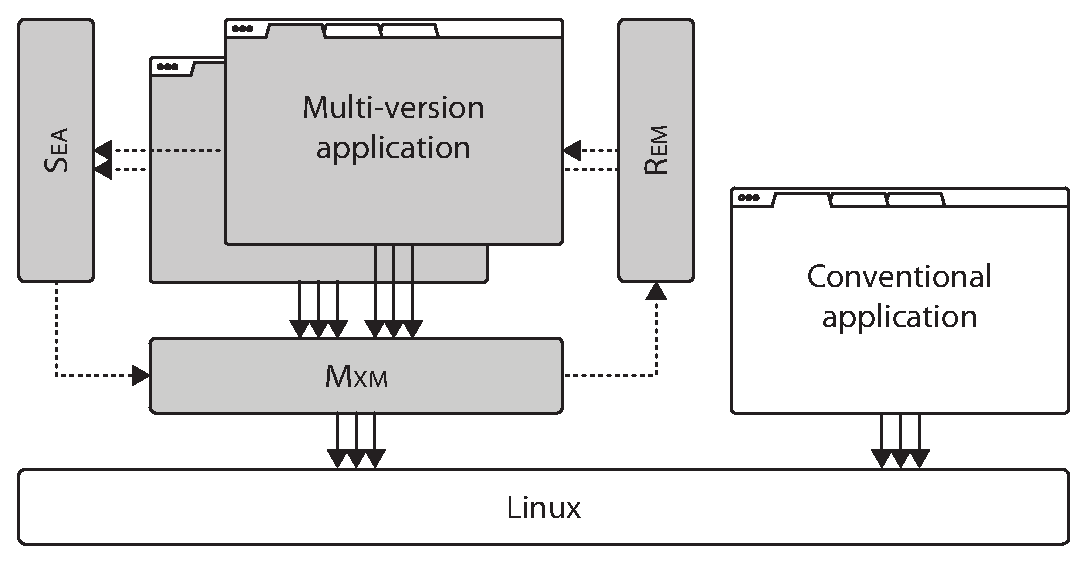
\includegraphics[width=0.6\columnwidth]{safe-updates/figures/architecture}
\caption{\mx system architecture.  
%% The main components of \mx
%%   are \sea (Static Executable Analyser), \mxm (Multi-eXecution
%%   Monitor), and \rem (Runtime Execution Manipulator).
}
\label{fig:design}
\end{center}
\end{figure}


\subsection{System call interposition}
\label{sec:mxm}

One of the main components of our multi-version execution environment
is the \mxm monitor.  \mxm's main jobs are to run the two versions
concurrently, mediate their interaction with the outside world,
synchronise their executions, and detect any divergences in their
external behaviour. \mxm works by intercepting all system calls issued
by each application version, and manipulating them to ensure that the
two versions are executed in a synchronised fashion and act as one to
the outside world.

\mxm provides functionality similar to conventional virtual machine monitors.
Whenever the MV application is executed, the \mxm connects to the two
application versions running in parallel, intercepting their kernel system
calls.  \mxm ensures that the two versions act as one to the outside world by
mediating access to the underlying operating system to achieve complete
isolation of the running application from other application instances as well
as from the external environment, making sure the combined application versions
act as one to the outside world.  The environment controlled by the monitor
consists mainly of a restricted file system access, socket interceptors and
signal handlers.

\subsubsection{System call interception}

\mxm is implemented using the  \ptrace interface provided by the Linux
kernel.  This interface, often used for application debugging, allows
simple deployment (without any need for compile-time instrumentation)
and makes the monitor itself lightweight since it is running as a
regular unprivileged process.  \mxm is similar in operation to previous
monitors whose goal is to synchronise applications at the level of system
calls such as \orchestra~\cite{orchestra09}, PLR~\cite{shye2009} or
\tachyon~\cite{tachyon12}.

\mxm runs each version in a separate child process, intercepting all
their system calls.  When a system call is intercepted in one version,
\mxm waits until the other version also performs a system call.  With
a pair of system calls in hand (one executed by the old version, and
one by the new version), \mxm compares their types and arguments.  If
they differ, \mxm has detected a divergence and invokes the \rem
component to resolve it (\S\ref{sec:rem}).

Otherwise, if the two versions perform the same system call with the
same arguments, \mxm virtualises their interaction with the
environment.  If the operation performed by the system call has no
side effects and does not involve virtualised state (\eg
\lstinline`sysinfo`), \mxm allows both processes to execute it
independently.  Otherwise, it executes the system call on their
behalf and copies its results into the address spaces of both
versions.

\mxm must also enforce deterministic execution across versions. This
consists mainly of intercepting instructions that may produce
non-deterministic results, and returning the same result in both
versions.  Examples of such non-deterministic operations include
random number generators (\eg read calls to \lstinline`/dev/[u]random`),
date and time (\eg read calls to \lstinline`/etc/localtime`), and access
to files and network (\eg file descriptor consistency).  Note that
non-deterministic effects resulting from allocating memory objects at
different addresses in memory or randomly arranging memory areas via
address space layout randomisation (ASLR) do not pose any
problems: \mxm understands the semantics of individual system calls and
rather than directly comparing memory addresses (which might be
different in each executed version), it compares the actual values
stored at those memory locations. \mxm supports both memory buffers (by
comparing the actual buffer content) as well as data structures
referenced by pointers (including nested ones).
 
Since \mxm fully controls executing programs intercepting all their system
calls, it can ensure that both programs have the same view of their
environment. Whenever the monitored process makes a system call, \mxm is
notified twice---first before, then after the call has been executed.  When a
\ptrace event is raised (\eg a new child process has been started), the monitor
is notified as well.  Due to internal limitations of the \ptrace interface,
once the system call has been made, it cannot be skipped, so when \mxm wants to
execute the call on behalf of its child processes, it simply replaces it with a
system call that does not change the system state (\lstinline`getpid` in our
case).

There are several challenges that we encountered while implementing
\mxm.  First, \mxm must partly understand the semantics of 
system calls.  For example, many system call parameters use complex
(often nested) structures with complicated semantics to pass values to
the operating system kernel, as in the case of \lstinline`ioctl` or
\lstinline`futex`.  To be able to compare the parameters of
these system calls and copy back their results, \mxm needs to
understand the semantics of these structures.  However, there are only
a relatively small number of system calls in Linux, and once the support
for handling them is implemented, it can be reused across applications.
\mxm currently implements \syscallsImplemented system calls (out of the
\syscallsTotal provided by Linux x86-64 3.1.9), which was enough to
allow us to run \mx on our benchmarks
(\S\ref{sec:reliability-evaluation}).

Second, the arguments of a system call are often passed through pointers,
which are only valid in the application address space, which is not directly
available to \mxm.  Therefore, \mxm needs to copy the contents pointed to by
these structures to its own address space in order to perform their
comparison.  The \ptrace interface on x86-64 only allows to copy one quadword
per system call, which is very expensive. Previous approaches either used
various ad-hoc optimisations~\cite{orchestra09} such as named pipes or shared
memory with custom shellcode, or a modified kernel~\cite{tachyon12} to
overcome this limitation. Instead, \mxm uses \emph{cross memory attach}, a new
mechanism for fast interprocess communication which has been recently added to
the Linux kernel~\cite{crossmemoryattach}.  This mechanism provides two new
system calls---\lstinline`process_vm_readv` and
\lstinline`process_vm_writev`---which allows the tracer to directly access the
memory space of the tracee using an interface similar to the \lstinline`readv`
and \lstinline`writev` system calls without any additional overhead.

Third, because the structures passed as arguments to system calls often have
variable size, \mxm also needs a fast way to allocate and deallocate memory
for them in order to minimise the overall overhead imposed by our system.  For
this purpose, \mxm uses a region-based memory allocator~\cite{memory-pools},
namely the \textsf{obstack}
library,\footnote{\url{http://www.gnu.org/software/hello/manual/libc/Obstacks.html}}
which is part of the \gnu C Library.  Each monitored process has its own
region, which is used for allocating memory to store the copy of the process'
system call arguments

\subsubsection{Multi-process and multi-threaded applications}

Finally, a particular challenge arises in the context of multi-process and
multi-threaded applications.  Using a single monitor instance to intercept both
versions and their child processes (or threads) would eliminate any advantage
that these applications derive from using concurrency.  Therefore, \mxm uses a
new monitor thread for each set of child processes (or threads) spawned by the
application.  For instance, if the old and new versions each have a parent and
a child process, then \mxm will use two threads: one to monitor the parent
processes, and one to monitor the child processes in each version.

Due to limitations of the \ptrace interface (which was not designed to be used
in a multi-process or multi-threaded environment), handing the control of any
child processes being spawned by the application over to a new monitoring
thread is somewhat complicated.  In \mxm we adopt a solution similar to
Orchestra~\cite{orchestra09}.  When a new child process is spawned, we let the
parent monitoring thread to supervise its execution until the first system
call.  Then, we replace this system call with a \lstinline`pause` system call,
disconnect the parent monitor (which causes a \lstinline`SIGCONT` signal to be
sent to all new child processes), and spawn a new monitoring thread which
immediately reconnects to the new child process, restores its original system
call, and resumes its execution.

\mxm does not enforce deterministic execution across multiple versions of
multi-threaded programs (which may diverge if race conditions can lead
to different external behaviour across executions), although we could
overcome this limitation by adopting \varan's solution
(\S\ref{sec:threading}).

%% \mxm also performs a series of optimisations to decrease performance
%% overhead, such as allowing certain files with read-only permissions
%% to be opened directly by the process. 

\subsubsection{Environment virtualisation}

To improve I/O performance and decrease virtualisation overhead,
processes are allowed to open files with read-only permissions
directly, while files with write permissions are opened by the monitor
itself.  This imposes another problem as file descriptors assigned to
these files are not necessarily the same in each version (\eg due to
scheduling non-determinism). Therefore, \mxm needs to virtualise
these file descriptors.

Whenever the monitored process opens a file with read-only permissions, a
new virtual file descriptor is assigned to this file together with the
mapping to a real file descriptor for each version. This virtual file
descriptor is then sent to each version. When a system call is made
using this virtual file descriptor, \mxm replaces it with the real
file descriptor before executing the system call. The actual file
operation is then executed by the process itself avoiding any memory
copying by \mxm.

A similar approach is also used for virtualisation of process,
group, parent and child identifiers.  Whenever a process tries to obtain
the actual ID, \mxm replaces this with a virtual ID and keeps the
mapping between the real and the virtual ID. When a process invokes a
system call using this ID as an argument (\eg \lstinline`kill`), the
virtual ID is replaced with the actual ID before executing the system
call.

%% \paragraph{Para-virtualisation interface and binary translation.}
%% Furthermore, we plan to combine this API with a binary translation
%% approach~\cite{binary-translation}, that will allow to dynamically
%% replace certain system calls with more efficient \emph{monitor
%% call} instructions.  The binary translation could be also used to
%% dynamically replace code components that have been proved to be
%% safe and do not need to be replicated across multiple versions (\eg
%% using static verification during compilation, using traces of
%% previous execution, using runtime heuristics).


%% \paragraph{Future work}

%% The \texttt{ptrace} interface allows us to easily monitor the program
%% execution without any compile-time instrumentation.  The main downside
%% of this approach is a relatively high overhead.  This is especially
%% true for I/O intensive applications, as they require frequent
%% transfers of large portions of the application memory space to the
%% monitor process. This overhead could be eliminated by directly
%% accessing the process memory space.

%% The existing prototype implementation of \textsc{Mxm} already supports
%% simple scenarios. The main limitation of this implementation is the
%% strict ordering of system calls, which must be the same in each
%% monitored application version.  To be practically usable, future
%% versions of \textsc{Mxm} need to relax the requirement on strict
%% ordering to allow more complex scenarios. This is especially important
%% when executing different versions of the same application.

%% Most importantly, a straightforward comparison of system call traces
%% is usually not sufficient to identify divergences, since different
%% versions might use a slightly different sequence of kernel and library
%% calls to implement the same behaviour.  We plan to explore approaches
%% similar to those implemented by compiler optimisations, such as
%% \emph{peep-hole optimisation}~\cite{dragon-book}, and adapt them to
%% work on the level of kernel and library calls.


%% %% \paragraph{Hashing system call traces.}
%% %% To decrease the overhead of kernel and library call synchronisation, we aim to
%% %% enhance our system to hash the sequence of system call traces using fast hash
%% %% functions such as FNV-1 or FNV-1a.  This approach has a significant advantage
%% %% over straightforward comparison of call traces, especially in the case of
%% %% system calls with virtually unlimited parameter sizes such as \texttt{read} or
%% %% \texttt{write}~\cite{shye2009}.  Similar approach has been already used
%% %% in~\cite{shye2009}.

%% \paragraph{Libraries support and virtualisation.}
%% Since many applications today use functionality provided by shared
%% libraries, we aim to support intercepting calls to such libraries as
%% well. Moreover, as intercepted calls to shared libraries can be
%% executed only once, same as in the case of system call monitoring,
%% this may decrease the overall overhead of multi-version execution.

%% We also plan to provide our own implementation of the \texttt{libc}
%% library loaded using the \texttt{LD\_PRELOAD} mechanism.  This library
%% will communicate directly with the monitor process through shared
%% memory, decreasing the number of system calls that need to be directly
%% intercepted, and thus resulting in much better performance.  However,
%% since the \texttt{LD\_PRELOAD} mechanism can be overridden, we still
%% need to combine it with the \texttt{ptrace} monitoring facility to
%% achieve complete isolation with reasonable overhead.  This approach
%% can be extended to support other shared libraries as well, further
%% improving the overall performance of our approach.

\subsection{Runtime state manipulation}
\label{sec:rem}

At the core of our system lies the \rem component, which is invoked
by \mxm whenever a divergence is detected.  \rem has two main jobs:
(1)~to decide whether to resolve the divergence in favour of the old or
the new version; and (2)~to allow the other version to execute through
the divergence and resynchronise the execution of the two versions
after the divergence.
%% The first task by itself it's easy: we favour the new version, except
%% for when it crashes.
%% As discussed in \sref{sec:scope}, in this paper we restrict our
%% attention to surviving crash errors, so the first task is relatively
%% easy: if one of the two versions crashes, we use the output of the
%% other version; otherwise, we always favour the new version.  
%%
%% The second task is however more difficult, but essential to the
%% success of our approach, which relies on having both versions be alive
%% at all times, so that the overall application can survive any crash
%% bugs that happen in either the old or the new version (although of
%% course, not in both).
%%
As discussed in Section~\ref{multi-version:rationale}, in \mx we focus
our attention on surviving crash errors, so the key challenge is to
allow the crashing version to survive the crash.  This is essential to
the success of our approach, which relies on having both versions alive
at all times, so that the overall application can survive any crash bugs
that happen in either the old or the new version (although of course,
not in both at the same time).

We emphasise that we apply our approach only to crash errors (those
raising a \lstinline`SIGSEGV` signal), and not to other types of program
termination, such as \lstinline`abort`.  This is important from a
security perspective, because
%% many patches turn potential compromises into
%% run-time {\small{\texttt{abort}s}}, \eg using assertions for input
%% sanitisation.  For example, 
when a vulnerability is discovered, but a proper solution is not yet
known, developers often\footnote{For example, see the patch in \texttt{json-cpp}~\url{http://jsoncpp.svn.sourceforge.net/viewvc/jsoncpp/trunk/jsoncpp/include/json/assertions.h?r1=247&r2=246&pathrev=247}}
fail-stop the program rather than letting it continue and allowing
the attacker to compromise the system.
%
%% Such situations can be easily distinguished since failed assertions
%% result in program abortion (\ie
%% \textstt{SIGABRT} signal), while unintentional program crashes typically
%% result in abnormal termination (\ie \textstt{SIGSEGV} signal). 
%% Therefore, \rem only intercepts and handles crashes resulting
%%   in \textstt{SIGSEGV} signals.

Suppose that one of the versions has crashed between the execution of
system call $s_1$ and the execution of system call $s_2$.  Then, in
many common scenarios, the code executed between the two system calls
is responsible for the crash (\eg the old version crashes because it
doesn't incorporate a bug fix present in the new version, or the new
version crashes because its code was patched incorrectly).  Therefore,
our strategy is to do a form of \textit{runtime code patching}, in
which we use the code of the non-crashing version to execute over the
buggy code in the crashing version.

%% If the behaviour of the two versions is different, but they both
%% continue to execute, then we favour the behaviour of the new version and
%% wait for the two versions to reconverge.

%% There are many different ways to achieve this goal, such as the use of
%% a mechanism based on check-pointing and roll-back~\cite{qin2005};
%% however, these mechanisms cannot deal with persistent errors which are
%% common in the case of software updates.

%% Our solution is based upon the observation that errors in programs are
%% usually located at particular places (\ie specific instructions) in
%% the program's code.  Therefore, we can use the code of the other, and
%% \ie correct, version to execute over this critical point in program's
%% code. This approach may not work when memory layout of the two
%% versions differs, as the code of one version may fail to locate the
%% memory structures necessary for its execution in the memory of the
%% other version. Nevertheless, the described approach might still work
%% in many cases when memory layout of the two versions does not differ
%% significantly.


%\paragraph{Possible execution scenarios.}

%% We run two versions of the same application in parallel, monitoring
%% their execution to be sure that they behave in the same way without
%% any divergences by comparing the application executions at
%% synchronisation points; in case of our prototype equal to system
%% calls. When either of the versions fail, we stop its execution at the
%% \emph{divergence point}; at this point there are three possible
%% solutions to synchronise the divergent versions:

\begin{figure}[t]
\centering
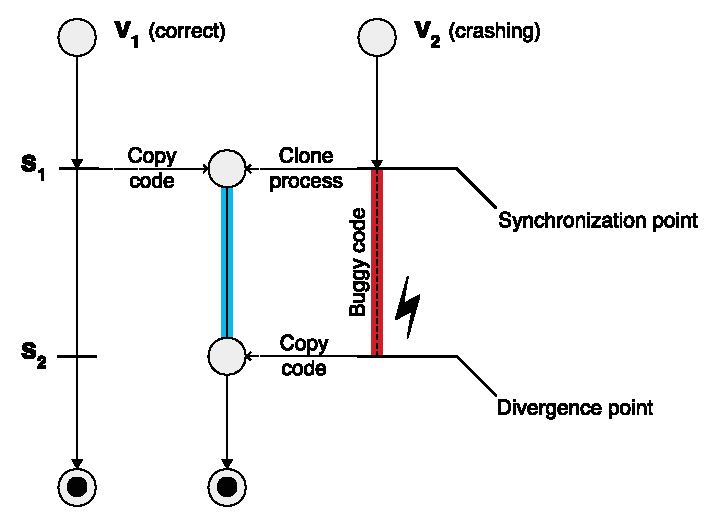
\includegraphics[width=0.5\columnwidth]{safe-updates/figures/strategy}
\caption{\rem's recovery mechanism uses the code of the non-crashing
  version to run through the buggy code.}
\label{fig:solution3}
\end{figure}

%% \begin{enumerate}[label=\emph{S\arabic*}, itemsep=3pt, parsep=3pt]
%% \renewcommand*\labelitemi{\emph{S\arabic*}}
%% \begin{figure}[t]
%%   \centering
%%   \subfloat[Patch state after the crash and continue execution]{
%%     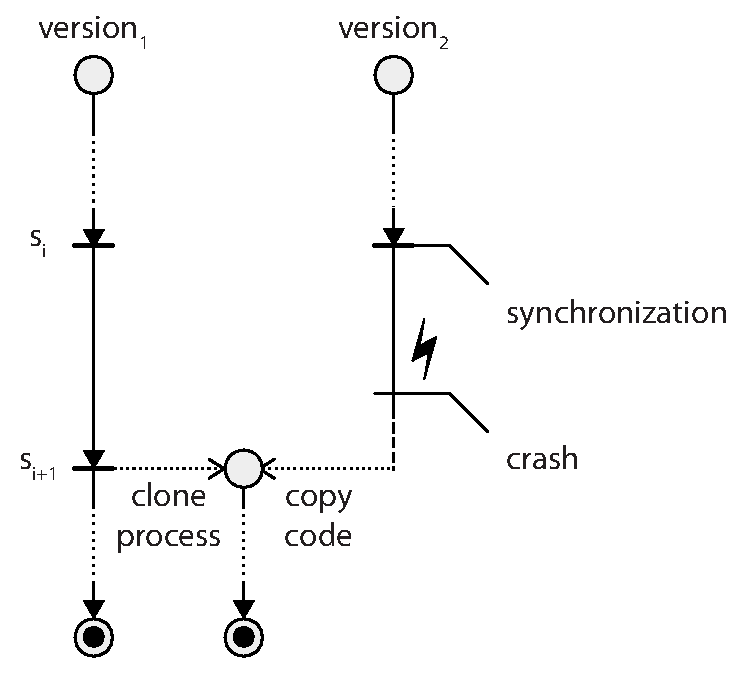
\includegraphics[width=0.45\columnwidth]{safe-updates/figures/solution1}
%%     \label{fig:solution1}
%%   }
%%   \quad
%%   \subfloat[Patch state before the crash and continue execution]{
%%     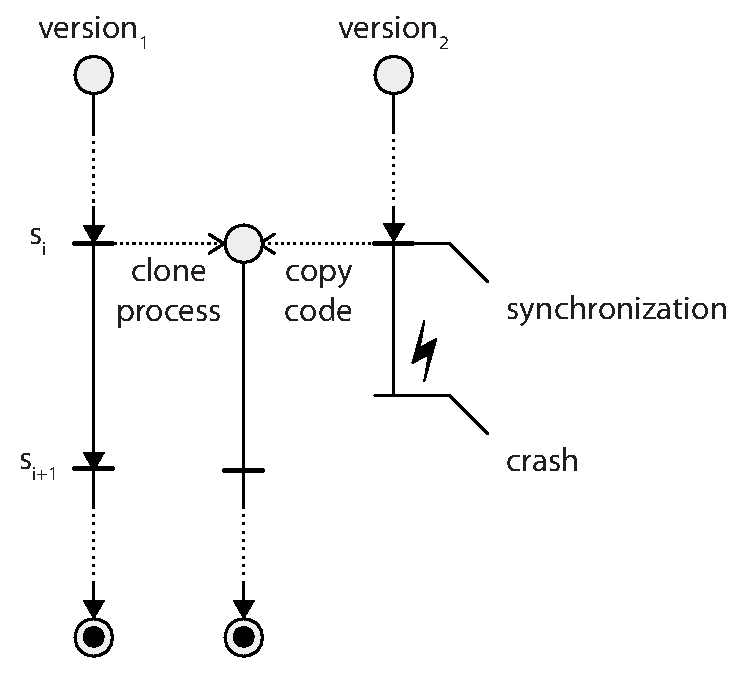
\includegraphics[width=0.45\columnwidth]{safe-updates/figures/solution2}
%%     \label{fig:solution2}
%%   }
%%   \\
%%   \subfloat[Use the code of older version only to run through critical section]{
%%     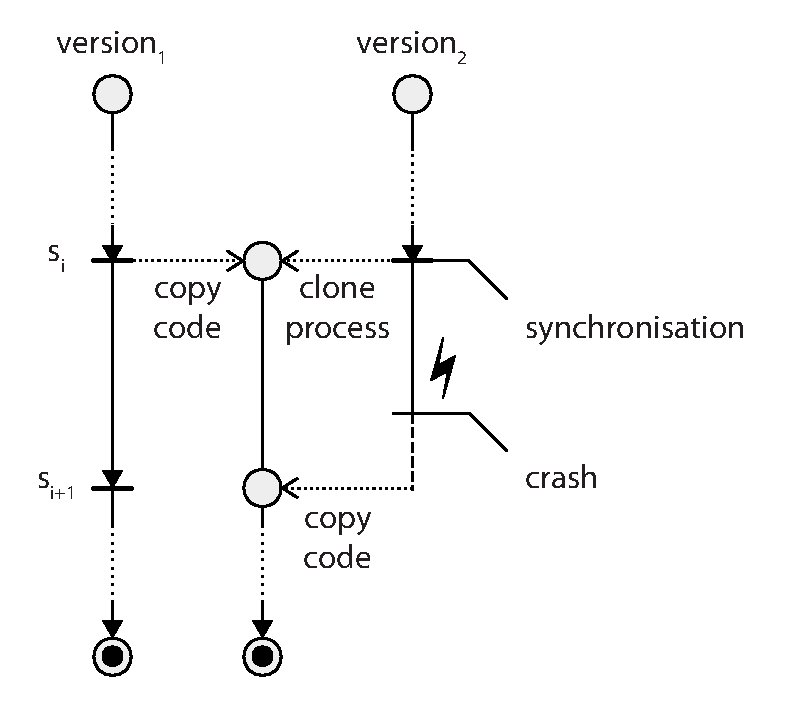
\includegraphics[width=0.45\columnwidth]{safe-updates/figures/solution3}
%%     \label{fig:solution3}
%%   }
%%   \caption{Three solutions for synchronising two divergent versions of
%%   the same application}
%%   \label{fig:solution}
%% \end{figure}

%% \item\label{s1} Clone the correctly executing version to duplicate its state
%%   (\eg memory content, memory mappings) after the crash and replace its
%%   code with the code of the failed version. Then restart both versions and
%%   continue their execution (Figure~\ref{fig:solution1}).

%% \item\label{s2} Clone the correctly executing version to duplicate its state
%%   (\eg memory content, memory mappings) at the last synchronisation point (\ie
%%   creating checkpoint). After the crash, replace the code of this cloned
%%   version with the code of the failed version. Then restart this cloned
%%   version, execute over the \emph{critical section}, and continue execution of
%%   both versions (Figure~\ref{fig:solution2}).

%% \item\label{s3} Clone the failing version to duplicate its state (\eg memory
%%   content, memory mappings) at the last synchronisation point (\ie creating
%%   checkpoint). After the crash, replace the code of this cloned version with
%%   the code of the correctly executing version. Then restart this cloned
%%   version; after the application successfully executes over the \emph{critical
%%   section}, replace the code of the cloned version again with the original
%%   code, and continue its execution (Figure~\ref{fig:solution3}).

%% \end{enumerate}

Our exact recovery mechanism is illustrated in
Figure~\ref{fig:solution3}.  At each system call, \mx creates a
lightweight checkpoint of each version.  This is implemented using the
\lstinline`clone` system call in Linux, which internally uses a
copy-on-write strategy.  
%% As an important optimisation, we omit system
%% calls that can be replayed safely from the last checkpoint, such
%% as \textstt{read}.

As shown in Figure~\ref{fig:solution3}, suppose that the crash happens in
version $v_2$, between system calls $s_1$ and $s_2$.  Then, \rem first restores
$v_2$ at point $s_1$ (\circl{A}), copies $v_1$'s code into $v_2$'s code segment
(\circl{B}), executes over the buggy code using $v_1$'s code (\circl{C}, note
that we are still using $v_2$'s memory state), and then restore $v_2$'s code at
point $s_2$ (\circl{D}).

There are several challenges in implementing this functionality.
First, \rem needs the ability to read and write the application's code
segment.  In the current implementation, we bypass this by linking
together the two application versions after renaming all the symbols
in one of the versions using a modified version of
the \texttt{objcopy}
tool.\footnote{\url{http://sourceware.org/binutils/docs/binutils/objcopy.html}}
However, in the future we plan to implement this transparently by
using the cross-memory attach mechanism used by \mxm.
%% \textstt{pread} and \textstt{pwrite} interface to directly
%% read and write the process memory via the
%% %\textstt{/proc/<pid>/mem} file in the
%% \emph{proc} file system.

%% This functionality has been recently introduced to the Linux kernel in
%% version 2.6.39~\cite{kernel-procmem}; previously, this interface was
%% read-only. This approach imposes only minimal overhead as it allows
%% direct access to the process memory space.

%% The runtime process manipulation functionality is implemented inside
%% \rem, a separate component used by the \mxm monitor. The
%% manipulation itself is driven by the data obtained statically by the
%% \sea analyser before the application has been executed.

Second, \rem needs to modify the contents of the stack in $v_2$.  This is
necessary because the return addresses on the stack frames of $v_2$ still point
to $v_2$'s original code, which was now replaced by $v_1$'s code.  Without also
modifying $v_2$'s stack, any function
\lstinline[language={[x64]Assembler}]`RET` instruction executed between $s_1$
and $s_2$ would most likely veer execution to an incorrect location, since
function addresses are likely to be different across different versions.  Thus,
after \rem replaces $v_2$'s code, it also updates the return addresses on
$v_2$'s stack with the corresponding return addresses in $v_1$, which are
obtained via static analysis (\S\ref{sec:sea}).  Because system calls are
invoked via wrapper functions in C library, this ensures that when $v_2$
resumes execution, it will immediately return to the code in $v_1$.
%% \rem obtains these addresses by analysing $v_1$'s stack at
%% position $s_1$ accessible via checkpoint taken at that point.
%
To implement this functionality, \rem makes use of
the \texttt{libunwind}
library,\footnote{\url{http://www.nongnu.org/libunwind/}} which provides a
portable interface for accessing the program stack, for both x86 and
x86-64 architectures. To actually modify the execution stack of
$v_2$, \rem uses again the \ptrace interface.


Unfortunately, updating the stack return addresses is not sufficient
to ensure that $v_2$ uses $v_1$'s code between $s_1$ and $s_2$, as
$v_2$ may also use function pointers to make function calls.
%% Note that we are still using the $v_2$ memory state. Thereby, $v_2$
%% may still issue a function call to the original code through one of
%% the function pointers.
To handle such cases, \rem inserts breakpoints to the first
instruction of every function in $v_2$'s original code.  Then, when a
breakpoint is encountered, \rem is notified via a \lstinline`SIGTRAP`
signal, and redirects execution to the equivalent function in $v_1$'s
code (which is obtained from the \sea component) by simply changing
the instruction pointer.
%The address of the equivalent function is obtained

Finally, after executing through the buggy code, \rem performs the
same operations in reverse: it redirects execution to $v_2$'s original
code, changes the return addresses on the stack to point to $v_2$'s
functions, and disables all breakpoints inserted in $v_2$'s code.  
The one additional operation that is done at this point is to copy all
the global data modified by $v_1$'s code into the corresponding
locations referenced by $v_2$'s code.  

%\paragraph{Runtime stack analysis and manipulation.}

%% For example, on the x86 architecture, the stack can be easily
%% traversed starting from the top as each stack frame contains frame
%% pointer pointing to the previous stack frame, thereby forming a linked
%% list-like structure. This is not possible on the x86-64 architecture
%% as the frame pointer is no longer stored inside the stack frame.  To
%% traverse the execution stack on this architecture, it is necessary to
%% compute sizes of all functions' stack frames using the stack usage
%% information stored in the \texttt{UNWIND\_CODE} section, which is a
%% part of the ELF binary file. This logic is implemented by the
%% \texttt{libunwind} library, which provides API to unwind the stack
%% independent of the target platform.

%The necessary information about the stack location (\ie address range) and
%page mapping are obtained through the \emph{proc} file system; in particular
%the \textstt{/proc/<pid>/maps} and \textstt{/proc/<pid>/pagemap} files.

Note that \mx cannot currently handle major modifications to the
layout of the data structures used by the code, including individual
stack frames.  While this still allows us to support several common
software update scenarios, in future work we plan to improve the
system with the ability to perform full stack
reconstruction~\cite{upstare} and automatically infer basic data
structure changes at the binary-level~\cite{data-struct-digging}.
%% to identify changes to function names and sequences of function calls
%% (e.g., via clone detection techniques~\cite{cp-miner06,deckard07}),


Our approach of using the code of the non-crashing version to survive failures
in the crashing version may potentially leave the recovered version in an
inconsistent state. However, \mx is able to discover most internal state
inconsistencies by checking whether the two versions have the same external
behaviour after recovery. When the behaviour of the recovered version starts to
differ, \mx will immediately discard it and continue with only one version. The
discarded version can be later restarted at a convenient synchronisation point.
This restarting functionality is not currently implemented in \mx, but we plan
to add it as a future extension.

%Our approach of using the code of the non-crashing version to survive
%failures in the crashing one may leave the application in an
%inconsistent state, and thus may not be applicable for application in
%which absolute correctness and a fail-fast approach are more important
%than allowing the application to survive errors.  However, \mx is
%usually able to discover most internal state inconsistencies, since it
%regularly checks if the two versions have the same external
%behaviour. (See \S\ref{sec:discussion} for an extended discussion.)

\subsection{Binary static analysis}
\label{sec:sea}

%% \begin{table*}[t]
%% \centering 
%% \begin{tabular}{ccc}
%%   \hline
%%   Library calls in $\mathrm{version}_1$ & Library calls in $\mathrm{version}_2$ &
%%   System calls within the library \\
%%   \hline
%%   \texttt{<0xdeadbe5a>} & \texttt{<0xdeadbe8e>} &
%%   [\texttt{<0x77ff2c>}, \texttt{<0x77ffae>}] \\
%%   \texttt{<0xdeadabf5>} & \texttt{<0xdeadac34>} &
%%   [\texttt{<0x782bae>}] \\
%%   \vdots & \vdots & \vdots \\
%% \end{tabular}
%% \caption{Addresses of library function calls, and system calls invoked from
%% within these functions.}
%% \label{tab:syscall_table}
%% \end{table*}

The \sea component statically analyses the binaries of the two
versions to obtain information needed at runtime by the \rem
component.  \sea is invoked only once, when the multi-version
application is assembled from its component versions.
%% As mentioned in \sref{sec:rem}, we currently link together the
%% two application versions after renaming all the symbols in one of them
%% using a modified copy of the \textstt{objcopy} tool, although in the
%% future we plan to do this linking dynamically by directly changing the
%% code segment in each version.

The main goal of \sea is to create several mappings from the code of
one version to the code of the other.  First, \sea extracts the
addresses of all function symbols
in one version and maps them to the
addresses of the corresponding functions in the other version.  This
mapping is used by \rem to handle calls performed via function
pointers (\S\ref{sec:rem}).

Second, \sea computes a mapping from all possible return addresses in
one version to the corresponding return addresses in the other version.  In
order to allow for code changes, this mapping is done by computing an
ordered list of all possible return addresses in each function.  For
example, if function \lstinline`foo` in $v_1$ performs call instructions
at addresses \lstinline`0xabcd0000` and \lstinline`0xabcd0100`, and
function \lstinline`foo` in $v_2$ performs call instructions at
addresses \lstinline`0xdcba0000` and \lstinline`0xdcba0400`, then \sea
will compute the mapping \texttt{\{0xabcd0005 $\rightarrow$
0xdcba0005, 0xabcd0105 $\rightarrow$ 0xdcba0405\}} (assuming each call
instruction takes 5 bytes).  This mapping is then used by \rem to
rewrite return addresses on the stack.

%% These data are gathered by the \sea analyser component which
%% implements static analysis of binary executables to extract all
%% necessary addresses and provide them to other components inside our
%% system. The format used for storing these data is represented by a
%% \emph{call table}. For each version, this table contains addresses of
%% all calls to shared library functions together with the list of all
%% system calls addresses invoked within these library functions, as can
%% be seen in Table~\ref{tab:syscall_table}.

%% For example, the first line of this table represents a call to a
%% library function which does two system calls, while second line
%% represents a function call which does only one system call.

To construct these tables, \sea first needs to extract the addresses
of all function symbols and then disassemble the code for each
individual function in order to locate the call instructions within
them.  The implementation is based on the \texttt{libbfd}
and \texttt{libopcodes} libraries, which are 
part of the
\gnu \binutils suite.\footnote{\url{http://www.gnu.org/software/binutils/}}
To obtain the addresses of all function symbols defined by the
program, \sea uses \texttt{libbfd} to extract the static and dynamic
symbol tables and relocation tables.  To disassemble individual
functions, \sea uses the \texttt{libbf}
library~\cite{kwan:libbf}, built on top of \texttt{libopcodes}.

%% Disassembled machine code is stored in a graph-like structure where
%% individual instructions represents vertices and edges between these
%% vertices represents the control flow. 

%% \paragraph{System call identification.}
%% \sea implementation uses the disassembler to obtain machine
%% code of each individual function and iterates over its instructions
%% (traversing the instruction graph) to identify basic blocks and locate
%% system call instructions within the code these functions.

%% To locate system calls within shared library function calls,
%% \sea first needs to obtain the set of exported library
%% functions and system calls within these functions using the above
%% described approach. Then, \sea analyses the application binary
%% itself and locates all function calls to the shared library using the
%% information extracted from relocation and procedure lookup tables
%% contained in ELF binaries.

%% Results of this analysis are stored in a hash table and tree structure
%% to allow quick access eliminating any unnecessary overhead when these
%% information are accessed during runtime. These data are then used to
%% construct the already described \emph{call table}, before the
%% application itself is executed.

%% \subsection{Limitations and Future Work}
%% \label{sec:limitations}
%% \input{limitations}


\section{Reliability Evaluation}
\label{sec:reliability-evaluation}
\section{Reliability Evaluation}
\label{sec:reliability-evaluation}

To evaluate our approach, we show that \mx can survive crash bugs in several
real applications (\S\ref{sec:surviving}). We then examine the question of how
far apart can be the versions run by \mx (\S\ref{sec:bounds}), and discuss
\mx's performance overhead (\S\ref{sec:performance}).

\subsection{Fault recovery}
\label{sec:surviving}

We have evaluated \mx using a set of bugs in three applications: \gnu
\coreutils, \redis and \lighttpd. We discuss each application in turn below.

\subsubsection{\gnu \coreutils}
\label{sec:coreutils}

\begin{table}[t]
\begin{center}
\caption{Utilities from \gnu \coreutils, the crash bugs used, and the 
versions in which these bugs were introduced and fixed.  We group
together utilities affected by the same or similar bugs.}
\begin{tabular}{lll}
\toprule
\textsc{Utility} & \textsc{Bug description} & \textsc{Bug span} \\
\midrule
\mdsum & \multirow{2}{*}{Buffer underflow} & \multirow{2}{*}{v5.1 -- v6.11} \\
\shasum & & \\
\midrule
\mkdir & \multirow{2}{*}{\textstt{NULL}-pointer dereference} & \multirow{2}{*}{v5.1 -- v6.11} \\
\mkfifo & & \\
\mknod & & \\
\midrule
\cut & Buffer overflow & v5.3 -- v8.11 \\
\bottomrule
\end{tabular}
\label{tbl:cu-bugs}
\end{center}
\end{table}

As an initial evaluation of \mx's ability to survive crashes, we have used
applications from the \gnu \coreutils utility
suite,\footnote{\url{http://www.gnu.org/software/coreutils/}} which provides
the core user-level environment on most UNIX systems.  We have selected a
number of bugs reported on the \coreutils mailing list, all of which trigger
segmentation faults.  The bugs are described in Table~\ref{tbl:cu-bugs},
together with the utilities affected by each bug and the versions in which they
were introduced and fixed.

The bug affecting both \mdsum and \shasum utilities introduced in 5.1 and later
fixed in 6.11 caused a crash due to buffer underflow when checking an invalid
BSD-style input. Another bug we have considered affected \mkdir, \mkfifo and
\mknod utilities; this bug, which was reported in 6.10 and fixed in 6.11
resulted in crash when diagnosing invalid context.  Finally, the bug affecting
\cut utility, introduced in 5.3 and later fixed in 8.11, resulted in segfault
when using large unbounded range. 

For all these bugs, we configured \mx to run the version that fixed the bug
together with the one just before.  (we could have also run the version that
introduced the bug with the one just before, but we could not immediately tell
where the bug was introduced, and we cannot build versions earlier than 6.10
due to changes in GCC and GNU C library).  \mx successfully intercepted the
crash and recovered the execution by using the strategy described in
\sref{sec:rem}.

We discuss below the bug in the \cut utility (used to remove sections from each
line of file), triggered by the following invocation:

\begin{lstlisting}[numbers=none,breaklines=true,xleftmargin=0pt,language=bash]
cut -c1234567890- --output-d=: foo
\end{lstlisting}

This bug is triggered by the conditional statement on line~\ref{line:cond}:

\begin{lstlisting}[firstnumber=525]
if (output_delimiter_specified /*@\label{line:cond}@*/
    && !complement
    && eol_range_start && !is_printable_field (rsi_candidate))
\end{lstlisting}

This code uses the lower bound of the size of the printable field
vector; however, when calculating the size of this vector, ranges going
to the end of line (\ie \lstinline`0-`) are not considered eventually
resulting in invalid memory access. 
% The bug is caused by a buffer overflow whose root cause is the
% incorrect calculation of the size of a dynamically allocated buffer
% used internally by \cut.
When \mx intercepts this bug, it uses the
last checkpoint to recover the execution of the crashing version. This
checkpoint is taken after the \textstt{brk} system call triggered by
the \textstt{malloc} call that allocates the buffer. 
% in function \textstt{bindtextdomain} on line~\ref{line:bind}.
% \begin{lstlisting}[firstnumber=767]
% bindtextdomain (PACKAGE, LOCALEDIR); /*@\label{line:bind}@*/
% \end{lstlisting}
The recovered process uses the code of the other version to correctly
calculate the size of the field vector and switches back to the original
code during the allocation of this buffer as
%code during the allocation of this buffer on line~\ref{line:alloc} as
function \textstt{xzalloc} triggers \textstt{mmap64} system call, just
before executing the conditional statement on line~\ref{line:cond},
which originally triggered the bug.

\subsubsection{\redis}
\label{sec:redis}

Below, we describe how \mx can survive the \redis bug described in
Section~\ref{multi-version:scenarios} while running in parallel the \redis
revision \textstt{a71f072f} (\textit{the old version}, just before the bug was
introduced) with revision \textstt{7fb16bac} (\textit{the new version}, just
after the bug).  \mx first invokes \sea to perform a static analysis of the two
binaries and construct the mappings described in \sref{sec:sea}.  Then, \mx
invokes the \mxm monitor, which executes both versions as child processes and
intercepts their system calls.

When the new version crashes after issuing the problematic
\textstt{HMGET} command, \mxm intercepts the \textstt{SIGSEGV} signal
which is sent to the application by the operating system.  At
this point, \rem starts the recovery procedure.  First, \rem sends a
\textstt{SIGKILL} signal to the new version to terminate it.  It then
takes the last checkpoint of the new version, which was taken at the
point of the last invoked system call, which in this case is an
\textstt{epoll\_ctl} system call.  Then, \rem uses the information
provided by \sea to rewrite the stack of the new version, as detailed
in \sref{sec:rem}.  In particular, \rem replaces the return
addresses of all functions in the new version with the corresponding
addresses from the old version. The stack rewriting itself however is not
enough. The newer version can still use function pointers, which are part of
the replica state, to invoke the original code. To prevent this situation, \rem
inserts breakpoints at the beginning of all the functions in the code of the
new version (to intercept indirect calls via function pointers), and then
finally restores the original processor registers of the checkpointed process
and restarts the execution of the (modified) new version.

Since the checkpoint was performed right after the execution of the system
call \textstt{epoll\_ctl}, the first thing that the code does is to
return from the \textstt{libc} wrapper that performed this system
call.  This in turn will return to the corresponding code in the old
version that invoked the wrapper, since all return addresses on the
stack have been rewritten.  From then on, the code of the old version
is executed (but in the state of the new version), until the first
system call is intercepted.  In our example, the old and the new
versions perform the same system call (and with the same arguments),
so \rem concludes that the two processes have re-converged, and thus
restores back the code of the new version by performing the steps
above in reverse, plus the additional step of synchronising their
global state (see \S\ref{sec:rem}).  Finally, the control is handed
back to the \mxm monitor, which continues to monitor the execution of
the two versions.

\subsubsection{\lighttpd}
\label{sec:lighttpd}

To evaluate \mx on \lighttpd, we have used two different crash bugs.
The first bug is the one described in detail in
Section \ref{multi-version:scenarios}, related to the ETag and compression
functionalities.  As previously discussed, the crash is triggered by a
very small change, which decrements the upper bound of a \textstt{for}
loop by one.  \mx successfully protects the application against this
crash, and allows the new version to survive it by using the code of
the old version.

The other crash bug we reproduced affects the URL rewrite
functionality.\footnote{\url{http://redmine.lighttpd.net/projects/lighttpd/issues/2140}}
This is also caused by an incorrect bound in a \lstinline`for` loop.
More precisely, the loop: 

\begin{lstlisting}[numbers=none,breaklines=true,xleftmargin=0pt]
for (k=0; k < pattern_len; k++)
\end{lstlisting}

\noindent should have been:

\begin{lstlisting}[numbers=none,breaklines=true,xleftmargin=0pt]
for (k=0; k@+1@ < pattern_len; k++)
\end{lstlisting}

The bug seems to have been present since the very first version
added to the repository.  It was reported in December 2009, and
fixed one month later.  As a result, we are running \mx using the last
version containing the bug together with the one that fixed it.  While
this bug does not fit within the pattern targeted by \mx (where a
newer revision introduces the bug), from a technical perspective it is
equally challenging.  \mx is able to successfully run the two versions
in parallel, and help the old version survive the crash bug.

%The bug \#1601 affects the HTTP redirection functionality, in particular
%the \texttt{\%n} substitution with condition substring. This functionality has
%been introduced in revision \texttt{510}. However, there is an incorrect
%comparison in one of the conditions which causes segmentation fault when
%appending matched parts to buffer if there was no matching regular expression.
%The affected code can be seen in Listing~\ref{lst:510}.

%\begin{lstlisting}[label=lst:510, caption={Original correct version of the function}]
%cond_cache_t *cache = &con->cond_cache[dc->context_ndx];
%if (n > cache->patterncount) {
  %return 0;
%}
%\end{lstlisting}

%The fix to this bug consists of a single changed line as can be seen in
%Listing~\ref{lst:2138} and has been incorporated in revision \texttt{2138}, yet
%this bug remained undetected for nearly three years (August 8, 2005 --- March
%26, 2008) rendering \lighttpd webserver vulnerable to attack.

%\begin{lstlisting}[label=lst:2138, caption={Refactored failing version of the function}]
%cond_cache_t *cache = &con->cond_cache[dc->context_ndx];
%if (n >= cache->patterncount) {
  %return 0;
%}
%\end{lstlisting}

Both \lighttpd bugs \#1601 and \#2140 are very simple---their fix
consist of a single character---yet still they made \lighttpd server
vulnerable to a potential attack. \mx can not only handle the crash,
but also successfully recover the failing version in both cases.

\subsection{Ability to run distant versions}
\label{sec:bounds}

\begin{table}
\begin{center}
\caption{The maximum distance in number of revisions, and the time span
  between the revisions that can be run by \mx for each bug.}
\begin{tabular}{lcc}
\toprule
\textsc{Application Bug} & \textsc{Max distance} & \textsc{Time span} \\
\midrule
\lighttpd \#2169   & \maxDistLighttpdOne & \timeSpanLighttpdOne \\
\lighttpd \#2140   & \maxDistLighttpdTwo & \timeSpanLighttpdTwo \\
\redis \#344       & \maxDistRedis & \timeSpanRedis \\
%md5sum          & \maxDistMdsum & \timeSpanMdsum \\ \hline
\bottomrule
\end{tabular}
\label{tbl:bug-bounds}
\end{center}
\end{table}

In the previous sections, we have shown how \mx can help software
survive crash bugs, by running two \textit{consecutive} versions of an
application, one which suffers from the bug, and one which does not.
%
One important question is how far apart can be the versions run
by \mx.  To answer this question, we determined for each of the bugs
discussed above the most distant revisions that can be run together to
survive the bug.  

For the \coreutils benchmarks, we are able to run versions which are
hundreds of revisions apart: \maxDistMdsum~revisions (corresponding to
\timeSpanMdsum of development time) for the \mdsum/\shasum bug; 
\maxDistMkdir~revisions (\timeSpanMkdir of development time) for the 
\mkdir/\mkfifo/\mknod bug; and \maxDistCut~revisions (\timeSpanCut 
of development time) for the \cut bug.

The most distant versions for the first \lighttpd bug are
approximately two months apart and have \maxDistLighttpdOne~revisions
in-between, while the most distant versions for the second
\lighttpd bug are also approximately two months apart but have only
\maxDistLighttpdTwo~revisions in-between.  Finally, the most distant
versions for the \redis bug are \maxDistRedis~revisions
and \timeSpanRedis apart.  

Of course, it is difficult to draw any general conclusions from only
this small number of data points.  Instead, we focus on understanding
the reasons why \mx could not run farther apart versions for the bugs
in \lighttpd and \redis (we ignore \coreutils, for which we can run
very distant versions).
%% For the \coreutils bugs, the lower bound is the earliest
%% version that we could build and run on our machine (v6.10).  The
%% upper-bound for 
%
For \lighttpd issue \#2169, the lower bound is defined by a revision
in which a pair of \textstt{geteuid()} and \textstt{getegid()} calls
are replaced with a single call to \textstt{issetugid()} to
allow \lighttpd to start for a non-root user with GID~0.  \mx 
%cannot run this revision together with the one before it, because it 
currently does not support changes to the order of system calls, but we believe
this limitation could be overcome by using peephole-style
optimisations~\cite{dragon-book}, which would allow \mx to recognise
that the pair \textstt{geteuid()} and \textstt{getegid()} could be
matched with the call to \textstt{issetugid()}.  The upper bound
for \lighttpd issue \#2169 adds a \textstt{read} call to
\textstt{/dev/[u]random}, in order to provide a better entropy
source for generating HTTP cookies.  This additional \textstt{read}
call changed the sequence of system calls, which \mx cannot
handle. \looseness=-1

For \lighttpd issue \#2140, both the lower and the upper bounds are
caused by a change in a sequence of \textstt{read()} system calls.  We
believe this could be optimised by allowing \mx to recognise when two
sequences of read system calls are used to perform the same overall
read.

%% Lower bound: the fix consists of request parser changes which resulted
%% in different sequence of \textstt{read()} system calls. The different
%% sequence of \textstt{read()} calls also marked the upper bound in this
%% case, defined by revision \lighttpdTwoUB. In this revision, the way in
%% which input connection buffer is being filled has changed, fixing
%% issue \#2147 and CVE-2010-0295 vulnerability.

For the \redis bug, the lower bound is given by the revision in which the
\textstt{HMGET} command was first implemented.  Since there was no support for
\textstt{HMGET} before that version, \mx has no way to survive the crash caused
by invoking \textstt{HMGET} with a wrong type (see \S\ref{sec:redis}).  The
upper bound is defined by a revision which changes the way error responses are
being constructed and reported, which results in a very different sequence of
system calls.

%% , including the call on line
%% \ref{line:report-error2} in Listing~\ref{lst:refactored}, resulting in
%% different sequence of system calls.

%% \todo{explain that all of these changes are minor and some of them could be
%% very well handled by using window-based/peep-hole approach}

\subsection{Performance Overhead}
\label{sec:performance}

\begin{figure}[!t]
\centering
\includegraphics[width=\textwidth]{safe-updates/graphs/spec2006}
\caption{Normalised execution times for the \spec benchmark suite running under
\mx.}
\label{fig:spec}
\end{figure}

We ran our experiments on a four-core server with 3.50~GHz Intel
Xeon E3-1280 and 16~GB of RAM running 64-bit Linux v3.1.9.

\paragraph{\spec.}
To measure the performance overhead of our prototype, we first used
the standard \spec\footnote{\url{http://www.spec.org/cpu2006/}}
benchmark suite.  Figure~\ref{fig:spec} shows the performance of \mx
running two instances of the same application in parallel, compared to
a native system. The execution time overhead of \mx varies
from \minOverSPEC to \maxOverSPEC compared to executing just a single
version, with the geometric mean across all \numSPECbench benchmarks at
\avgOverSPEC. This result is comparable with previous work using multi-variant
execution that used SPEC CPU to measure performance~\cite{orchestra09} (even
though this work used SPEC~CPU2000 which has already been retired).

%% The overhead varies from \minRedisOver to \maxRedisOver depending
%% on the operation being performed. This is the worst case overhead
%% we have seen among all tested application and comes mainly from the
%% fact that \redis is an in-memory database optimised for maximum
%% bare-hardware performance and is very sensitive to any additional
%% software layers.  Even a state-of-the-art hypervisor can incur an
%% $n$-fold slowdown, so the relatively high measure overhead is
%% therefore unsurprising.

\paragraph{\gnu~\coreutils.} The six \coreutils applications discussed in 
\sref{sec:coreutils} are mostly used in an interactive fashion via the
command-line interface (CLI). For such applications, a high performance
overhead is acceptable as long as it is not perceptible to the user;
prior studies have shown that response times of less than 100ms
typically feel instantaneous~\cite{card:human_proc}. In many common use
cases (\eg creating a directory, or using \cut on a small text file),
the overhead of \mx was imperceptible---\eg creating a directory takes
around \avgMkdirNative natively and \avgMkdirMx with \mx. For the three
utilities that process files, we calculated the maximum file size for
which the response time with \mx stays under the 100ms threshold.  For
\cut, the maximum file size is \cutCutoffSize (with an overhead of
\cutCutoffOver), for \mdsum \mdsumCutoffSize (\mdsumCutoffOver
overhead), and for \shasum \shasumCutoffSize (\shasumCutoffOver
overhead).



\paragraph{\redis and \lighttpd.} To measure the performance overhead for \redis, 
we used
the \redisbenchmark\footnote{\url{http://redis.io/topics/benchmarks}}
utility, which is part of the standard \redis distribution and
simulates \textstt{GET}/\textstt{SET} operations done by $N$ clients
concurrently, with default workload.  For \lighttpd, we used the
\httpload\footnote{\url{http://www.acme.com/software/http_load/}}
multiprocessing test client that is also used by the \lighttpd
developers.  Both of these standard benchmarks measure the end-to-end
time as perceived by users.  As a result, we performed two sets of
experiments: (1) with the client and server located on the same
machine, which represents the worst case performance-wise for \mx; and
(2) with the client and server located on different continents (one in
England and the other in California), which represents the best case.

The overhead for \redis varies, depending on the operation being
performed, from \minRedisRemote to \maxRedisRemote in the remote
scenario, and from \minRedisOver to \maxRedisOver in the local
scenario.  The overhead for \lighttpd varies from \minLighttpdRemote
to \maxLighttpdRemote in the remote scenario, and
from \minLighttpdOver to \maxLighttpdOver in the local scenario.
Despite the relatively large overhead in the local experiments, the
remote overhead is negligible because times are dominated by the
network latency (which in our case is over $150$ms).

As a result, we believe \mx is most suitable for scenarios for which
its execution overhead does not degrade the performance of the
end-to-end task, such as the remote \redis and \lighttpd scenarios
discussed above, or interactive tasks such as those performed using
command-line utilities, where users would not notice the overhead as
long as the response time stays within a certain range.

%% \mx's performance overhead is strongly correlated with the frequency of
%% system calls that have to be intercepted.  Therefore, we could also
%% imagine \mx being automatically turned on and off during execution,
%% depending on the frequency of system calls experienced by the
%% application.

Finally, we would like to emphasise that our current prototype has not
been optimised for performance, and we believe its overhead can still
be significantly reduced.  
%% There are multiple strategies we plan to explore in future
%% work. First,
For example, we could synchronise versions at a coarser granularity,
by using an epoch-based approach~\cite{compl-schedules11}, or we could
improve our checkpointing mechanism by implementing it as a loadable
kernel module that only stores the part of the state needed for
recovery~\cite{flashback}.

%% and only checkpoint at epoch boundaries.  To make this approach viable, we also
%% need to record system calls in each epoch, so that they can be
%% replayed during recovery. Second, 

%% instead of using \textstt{clone}
%% directly, we could implement the checkpointing functionality as a
%% loadable kernel module and only store the part of the state needed for
%% recovery as in~\cite{flashback}. Finally, we could explore the
%% possibility of not intercepting system calls in certain parts of the
%% code that were previously shown to be safe and do not need to be
%% replicated across multiple versions (\eg similarly
%% to~\cite{onlinevalidation}).

%The measured overhead is higher than
%for the SPEC~CPU2006 benchmarks (with a slowdown of up to \maxRedisOver
%for some operations in \redis) and we are currently investigating the
%reasons for this slowdown.

%First, we could to synchronise versions at a coarser
%granularity, by using a window/epoch approach~\cite{compl-schedules11},
%and by performing certain synchronisations at the level of shared
%library calls.  Second, we could explore the possibility of not
%intercepting system calls in certain parts of the code that were
%previously shown to be safe and do not need to be replicated across
%multiple versions.  Finally, we could decrease the checkpointing
%overhead, by performing them at a lower frequency, and record the
%external behaviour since the last checkpoint, so that it can be
%successfully replayed during recovery (\eg as in Rx~\cite{rx}).

\begin{figure}[ht]
\begin{center}
\includegraphics[angle=270,width=\textwidth]{safe-updates/graphs/syscall}
\caption{Number of system calls made on average each second during the
execution of SPEC~CPU2006 benchmark suite, measured using \textstt{strace}
tool.}
\label{fig:syscall}
\end{center}
\end{figure}

We also examined how frequency of system calls affects the performance
overhead of application executed on top \mx. Figure~\ref{fig:syscall} shows
the average number of system calls during the execution of SPEC~CPU2006.
Rather surprising result is the fact that \textsf{452.libquantum}, even though having
the largest run time overhead had the lowest average number of system calls.
On the hand, the performance overhead of \textsf{400.perlbench}, despite having the
highest average number system, was bellow average. \todo{What is the conclusion here?}

% For example, as we discuss in related work, our
% monitor \mxm is very similar to the monitor used by
% Orchestra~\cite{orchestra09}, which by employing various optimisations
% manages to obtain an average overhead of only about 15\% when
% synchronising two program variants at the level of system calls.  In
% terms of checkpointing, the Rx system~\cite{rx} implements a similar
% approach based on the Linux copy-on-write mechanism, and which through
% various optimisations manages to achieve a performance penalty of less
% than 5\% when checkpointing every 200 milliseconds.


%\section{Introduction}
%\label{sec:intro}
%\input{safe-updates/intro}

%\section{Feasibility Study}
%\label{sec:evolution}
%\chapter{Software Evolution in Real-world}
\label{chap:evolution}

The multi-version execution approach is based on two key assumptions.  First,
that new bugs are being introduced during software evolution and maintenance
process even to a well tested code. Second, that during software evolution,
the externally observable behaviour of the applications remains relatively
stable, especially between minor revisions (\ie security and bug fixes).  While
there is a lot of first hand and anecdotal evidence in support of these
assumptions, despite the key role that software evolution plays in the
application life cycle, it is surprising how few empirical studies one can find
in the research literature regarding the co-evolution of test suites and code
and their impact on the \emph{execution} of real systems.

Software repositories provide rich information about the construction and
evolution of software systems. While static data extracted from software
repositories have been extensively studied, dynamic metrics concerning the
execution of the software have received much less attention, due to the
inherent difficulty of running and monitoring a large number of software
versions.

In this chapter, we present an empirical study concerning dynamic metrics which
aims to answer some of the questions related to software evolution. To perform
this study, we have built a flexible infrastructure that can be used to run
each version of a system in isolation and collect static and dynamic software
metrics, using a lightweight virtualization environment based on software
containers, that can be deployed on a cluster of local or cloud machines.

We have used this infrastructure to examine how code and tests co-evolve in
\numSystems popular open-source systems. We report the main characteristics of
software patches, analyse the evolution of program and patch coverage, assess
the impact of non-determinism on the execution of test suites, and investigate
whether the coverage of code containing bugs and bug fixes is higher than
average.

% While static metrics can provide useful insights into the construction and
% evolution of software, there are many software engineering aspects which
% require information about software executions.  For example, the research
% community has invested a lot of effort in designing techniques for improving
% the testing of software patches, ranging from test suite prioritisation and
% selection
% algorithms~\cite{harrold:test-redundancy,test-pri,Rothermel96analyzingregression}
% to program analysis techniques for test case generation and bug
% finding~\cite{diff-symex,directed-test-augmen:09,express,directed-symex11,babic11,directed-incr-symex11,patch:spin12,interaction-changes13}.

% Many of these techniques depend on the existence of a manual test suite,
% sometimes requiring the availability of a test exercising the
% patch~\cite{onlinevalidation,tachyon12}, sometimes making assumptions about the
% stability of program coverage or external behaviour over
% time~\cite{cov_regr97,mx}, other times using it as a starting point for
% exploration~\cite{zesti,pretex,sage,test-augmentation:genetic-vs-concolic}, and
% often times employing it as a baseline for
% comparison~\cite{klee,dotnet-random-test08,semantic-fp-testing12,mutation-tests-oracle12}.
% However, despite the key role that test suites play in software testing, it is
% surprising how few empirical studies one can find in the research literature
% regarding the co-evolution of test suites and code and their impact on the
% \emph{execution} of real systems.

% In this chapter, we present \covrig, a flexible infrastructure that can be used
% to run each version of a system in isolation and collect static and dynamic
% software metrics, using a lightweight virtual machine environment that can be
% deployed on a cluster of local or cloud machines.

% We use \covrig to conduct an empirical study examining how code and tests
% co-evolve in \numSystems popular open-source systems.  We report the main
% characteristics of software patches, analyse the evolution of program and patch
% coverage, assess the impact of non-determinism on the execution of test suites,
% and investigate whether the coverage of code containing bugs and bug fixes is
% higher than average.

% We use \covrig to conduct an empirical study examining how programs evolve in
% terms of code, tests and coverage.  More precisely, we have analysed the
% evolution of \numSystems popular software systems with a rich development
% history over a combined period of \numYears years, with the goal of answering
% the following list of research questions (RQs):

% \begin{itemize}
% \item[\textssc{RQ1}] \textit{\rqone}
%             Are coding and testing continuous, closely linked
%             activities?  Or do periods of intense development
%             alternate with periods of testing?

% \item[\textssc{RQ2}] \textit{\rqtwo}
%             Are most code
%             patches accompanied by a new or modified test case?  How
%             many patches modify neither executable code nor tests?
           
% \item[\textssc{RQ3}] \textit{\rqthree}
%             Are most patches small?  
%             How many different parts of the code does a patch touch?
%             What is the median number of lines, hunks and
%             files affected by a patch?

% \item[\textssc{RQ4}] \textit{\rqfour}  Do tests fail non-deterministically?
%             Does running the test suite multiple times cover different
%             lines of code?

% \item[\textssc{RQ5}] \textit{\rqfive}
%             Does the overall coverage increase steadily over time, or
%             does it remain constant?  Are there revisions that
%             significantly increase or decrease coverage?

% \item[\textssc{RQ6}] \textit{\rqsix}
%             What fraction of a patch is covered by the regression test
%             suite?  Does patch coverage depend on the size of the
%             patch?

% \item[\textssc{RQ7}] \textit{\rqseven}  Are
%             tests exercising recent patches added shortly after the
%             patch was submitted?  If so, how significant is this
%             latent patch coverage?

% \item[\textssc{RQ8}] \textit{\rqeight}
%             Are most fixes thoroughly exercised by the regression
%             suite?  How many fixes are entirely executed?

% \item[\textssc{RQ9}] \textit{\rqnine}
%             Is code that contains bugs exercised less than other changes?
%             Is coverage a reasonable indicator of code quality? 

% %\item[\bf RQ10:] \textbf{Does buggy code have lower than average coverage?}
% \end{itemize}

\section{Study infrastructure}
\label{sec:design}

\begin{figure}[t!]
\centering
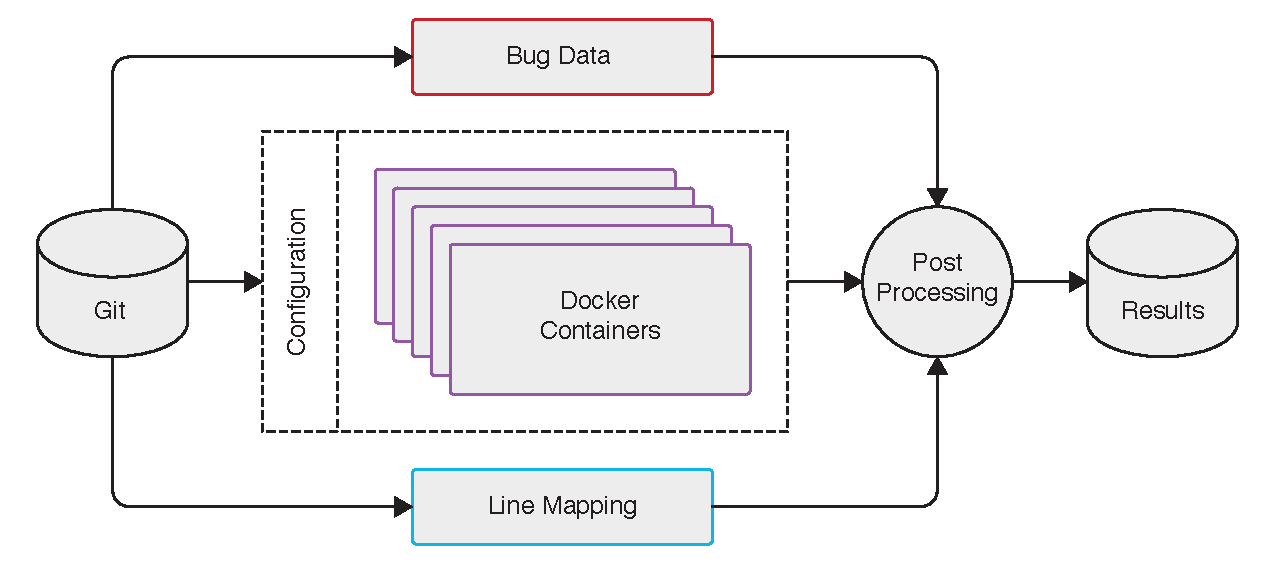
\includegraphics[width=0.75\textwidth]{evolution/figures/pipeline}
\caption{The architecture of the infrastructure used in the empirical study.}
\label{fig:arch}
\end{figure}

The overall architecture of the infrastructure used in our study is depicted in
Figure~\ref{fig:arch}.  It contains a generic driver which iterates through all
the revisions in a given range and invokes routines specific to each system to
compile, run, and collect statistics of interest.

%% To collect information about each program revision, such as whether it
%% successfully compiles, whether it passes the regression tests and with
%% what coverage, we built an infrastructure capable of automatically
%% retrieving and compiling each version of a target program, running
%% existing regression tests and collecting metrics of interest.

%The system is built on top of software containers~\cite{}, a
%lightweight virtualisation mechanism, which offers both isolation and
%reproducibility, by ensuring a consistent environment into which to
%run each software revision.  In this way, the execution of different
%revisions do not influence each other, \eg by inadvertently leaving
%behind lock files or not properly freeing up resources.

\paragraph{Lightweight software containers.} We employed software
containers~\cite{containers:eurosys07}, an operating system-level
virtualisation mechanism that provides the ability to run multiple isolated
virtual Linux systems (``containers'') inside a single host OS.  When launched,
the driver starts by loading the selected range of revisions from the project's
\git repository, and for each revision starts a new software container.  The
use of containers offers increased isolation and reproducibility guarantees by
providing a consistent environment in which to run each software revision and
ensuring that different revisions do not interfere with each other, \eg by
inadvertently leaving behind lock files or not properly freeing up resources.

The choice of lightweight OS-level virtualisation rather than more traditional
virtual machines (\eg \kvm\footnote{\url{http://www.linux-kvm.org/}} or
\xen\footnote{\url{http://www.xenproject.org/}}) reduces the performance
penalty associated with spawning and tearing down VMs, operations performed for
each revision analysed.  To get a sense of this difference, we compared an
\lxc\footnote{\url{http://linuxcontainers.org/}} container, which required
under a second for these operations, with a \xen VM, which needed over a
minute.

In our implementation, we use \docker\footnote{\url{https://www.docker.io/}} to
create and manage the lower-level \lxc containers, and
\vagrant\footnote{\url{https://www.vagrantup.com/}} to deploy them on multiple
local or cloud machines.  Each container is used to configure, compile and test
one program revision, as well as collect the metrics of interest, such as code
size and coverage. The containers are remotely controlled through SSH using the
\fabric\footnote{\url{http://fabfile.org/}} framework.

\paragraph{Configuration file.} We used a modular pipeline architecture, which
makes it possible to analyse new systems with modest effort. A potential user
of our infrastructure only needs to provide a Python configuration file
describing the system. A minimal file provides the name of the system, its \git
repository location, a method to compile the system, \eg install dependencies
and run the appropriate \stt{make} command, and a method to run the regression
tests, \eg run the \stt{make test} command.  Finally, the configuration file
can also specify an {\em end revision} and a specific number of revisions to
analyse.  For accurate test suite size measurements, the files or folders which
make up the test suite can also be indicated.

For each revision, we collect several static and dynamic metrics.  The static
metrics are obtained either directly from the version control system (\eg the
number of lines of test code) or after compiling each revision (\eg the number
of executable lines of code).  The dynamic metrics require running the
regression tests (\eg the overall line coverage or the regression test success
status).

Further information and graphs---including the ones presented in this
thesis---are automatically derived in the post-processing stage from these
primary metrics using a set of scripts.

%% For example, we were able to verify that the {\em latent patch
%% coverage}, \ie the fraction of code which is executed only several
%% revisions after it is introduced is small, and practitioners can
%% safely ignore it most of the time when evaluating test suite
%% augmentation or coverage-improvement techniques.

\paragraph{Bug data.} One possible application of our infrastructure is finding
useful data about software bugs and correlating them with the static and
dynamic metrics collected. For our study, we mined bug data from both software
repositories and, where available, bug tracking systems.  We automatically
obtained a list of candidate bug-fixing revisions by iterating through the list
of commits and checking the commit message for words such as {\em fix}, {\em
bug} or {\em issue}, followed by a number representing the bug identifier.  For
example, a typical \memcached bug fix commit message looks like {\em "Issue 224
- check retval of main event loop"}. The regular expression that we used to
identify these commits is similar to the ones used in prior
work~\cite{genealogies:issre13}:

\lstinline`(?:bug|issue|fix|resolve|close)\s*\#?\s?(\d+)`

Where possible, we confirmed that the bug identifier is valid by querying the
associated bug tracking system. We further manually checked all reported
revisions and confirmed that they included no false positives.  While it is
impossible to quantify the false negative rate without a knowledgeable
developer manually checking all the revisions in a repository, we believe that
the automatically obtained bug fixes create a representative subset of the
fixes in the repository.

\paragraph{Line mapping.} The ability to track how lines move and change
across revisions is the cornerstone of many high-level software
evolution analyses.  A line mapping algorithm improves over the
traditional \diff algorithm by tracking the movement of individual
lines rather than hunks.  Conceptually, line mapping is a function
which takes two revisions, \textit{r1} and \textit{r2}, and a program
location described by a pair \textit{(file name 1, line number 1)}
associated with \textit{r1}.  The output is a pair \textit{(file name
  2, line number 2)} identifying the corresponding location in
\textit{r2}.

Our implementation of the line mapping algorithm is similar to the
algorithms described in previous
work~\cite{szz:msr05,szz:ase06,change-source-code:msr07,szzrevisited:defects08}.
It makes use of the \emph{Levenshtein edit
  distance}~\cite{levenshtein1966binary} to track line edits, and
\emph{tf--idf}~\cite{tf-idf} and \emph{cosine
  similarity}~\cite{cosinesimilarity} to track line movements.  It
also uses the \emph{Hungarian algorithm}~\cite{hungarian} to find the
optimal matching of lines across versions.  Compared to previous work,
our implementation can also improve precision by using coverage information to filter
non-executable lines.

%% We used line mapping in two ways in our analysis: to determine whether
%% patches are tested within the next few revisions after they were
%% created (\S\ref{sec:lpcoverage}), and to estimate where bugs were
%% introduced (\S\ref{sec:bugs}).

In our study, we used line mapping to determine whether patches are
tested within the next few revisions after they were created
(\S\ref{sec:lpcoverage}).

\paragraph{Edit distance.} Edit distance, also known as Levenshtein edit
distance~\cite{levenshtein1966binary} is defined as a the minimum number of
operations (insertions, deletions, and subtitutions) required to transform one
string into the other. We use edit distance to measure the similarity of the
system call traces (\S\ref{sec:behavior-evolution}). However, these traces are
not strings, rather sequences of strings. To allow the use of edit distance on
these sequences, we use a hashing scheme, which assigns each string in the
sequence a 32-bit number. The algorithm then calulcates edit distance between
the integer strings.

Another problem is the efficiency of the implementation. The sequences we are
comparing in our study are hundreds of millions entries long. We have
implemented the Levenshtein algorithm as a native C Python extension and used
OpenMP to parallelize this implementation to take advantage of all available
cores. This implementation only keeps one line of the computation matrix, and
divides this line into strides which are then processed by different cores.

\paragraph{Cloud deployment.} To enable large-scale data collection and
processing, we deployed the infrastructure to our private cloud. We have built
our system around a standard set of tools: \packer for building custom
\docker-enabled machine images, \vagrant for controlling and provisioning the
virtual machines based on these images, a private \docker registry for serving
\docker containers containing the driver scripts, and a {\em fabfile} for
orchestrating the entire cluster. The same set of tools and scripts can be used
to deploy the infrastructure to different private or public clouds.

%% \subsection{High-Level Questions} \label{ssec:highlevel}

%% Coverage, bugs and line mapping data already provide useful insights into a
%% software project. For example, coverage and known bugs count can be used to
%% predict the residual bugs, i.e., the bugs still present in the software, using
%% a simple formula~\cite{coveragedefects98}

%% Using the bug data, we can quantify the number of patches which attempt to fix
%% a bug but either contain an incomplete fix or introduce new bugs. Such patches
%% are identified by looking for bug pairs, one being fixed and the other
%% introduced in the same patch. A high number of buggy fixes points to
%% deficiencies in the software development process.

%% \todo{More interesting things that we can do directly with coverage, bugs and
%% line mapping data}

%% However, further processing of this data allows us to answer more questions.
%% Combining  bug data and coverage data allows us to determine how many bugs are
%% in code which was already tested, i.e. executed without triggering the bug.
%% This may happen because the bug is only activated in corner-case scenarios.
%% Systems with a high number of bugs present in tested code may benefit from
%% symbolic execution-based testing tools such as ZESTI~\cite{zesti}, which
%% transparently instrument the existing tests to check for corner-case scenarios.
%% On the other hand, systems where the bugs are present in untested code can
%% benefit from test generation tools such as KATCH~\cite{katch}.

%% Correlations between bug data and software metrics can be used to build a bug
%% predictors based on project history and current patch coverage. Integrated in a
%% development environment or continuous integration system, such predictors can
%% warn developers when making high-risk changes. An intuitive predictor is based
%% on patch coverage: a tested patch is less likely to be buggy, compared to an
%% untested patch and the correlation can be mined from the project history. Code
%% churn can also be used as a predictor~\cite{churn-bugs:issre96, churndefects05}
%% and can be further refined to by eliminating non-executable changes or using
%% fine-grained souce code change extraction techniques~\cite{fluri:scc}
%% and its relationship with bugs can be mined using the line mapping data at the
%% line/function/file level.
%% % But we really don't want to go too much into statistics

%% Another question is whether old regression tests are still adequate for the
%% latest program version. We can quantify test adequacy by the fraction of the
%% code originally executed by the test that is still executed in the current
%% version. For an accurate computation we need to map the lines originally
%% executed to their counterparts in the current version.

\section{Study Setup}
\label{sec:study-setup}

We used the \covrig infrastructure to understand the evolution of
\numSystems popular open-source applications written in C/C++, over a
combined period of \numYears years. The six evaluated applications are:

\begin{enumerate}

\item[\gnu~\binutils\footnote{\url{http://www.gnu.org/software/binutils/}}]
is a set of utilities for inspecting and modifying object files,
libraries and binary programs.  We selected for analysis the twelve
utilities from the \stt{binutils} folder (\stt{addr2line}, \stt{ar},
\stt{cxxfilt}, \stt{elfedit}, \stt{nm}, \stt{objcopy}, \stt{objdump},
\stt{ranlib}, \stt{readelf}, \stt{size}, \stt{strings} and \stt{strip}),
which are standard user-level programs under many UNIX distributions.

\item[\beanstalkd\footnote{\url{http://kr.github.io/beanstalkd/}}]
is a simple and fast work queue originally designed for reducing the latency of
page views in high-volume web applications.

\item[\git\footnote{\url{http://git-scm.com/}}]
is one the most popular distributed version control systems used by the
open-source developer community.

\item[\lighttpd\footnote{\url{http://www.lighttpd.net/}}]
is a lightweight web server optimized for high performance environments.

\item[\lighttpdtwo\footnote{\url{http://redmine.lighttpdtwo.net/projects/lighttpdtwo2/}}]
is the new major version of the \lighttpd web server developed entirely from
scratch by the same team of developers.

\item[\memcached\footnote{\url{http://memcached.org/}}]
is a general-purpose distributed memory caching system used by several popular
sites such as Craigslist, Digg and Twitter.

\item[\redis\footnote{\url{http://redis.io/}}]
is a popular key-value data store used by many well-known services such as
Twitter, GitHub and StackOverflow.

\item[\zeromq\footnote{\url{http://zeromq.org/}}]
is a high-performance asynchronous messaging middleware library used by a
number of organisations such as Los Alamos Labs, NASA and CERN.

%\item {\bf GNU diffutils} is a collection of four widely-used
%programs: \stt{diff}, \stt{sdiff}, \stt{diff3} and \stt{cmp}, part of
%many popular UNIX distributions.

\end{enumerate}

The \numSystems applications are representative for C/C++ open-source
code: GNU \binutils are user-level utilities, \git is a version
control system, \beanstalkd, \lighttpdtwo, \memcached and \redis are server
applications, while \zeromq is a library.  All applications include a
regression test suite.

\begin{table}[t]
\caption{Summary of applications used in our study.
\textit{ELOC} represents the number of executable lines of code and
\textit{TLOC} the number of lines in test files in the last revision
analysed.}
\begin{center}
\begin{tabular}{llrlr}
\toprule
\multicolumn{1}{c}{}     & \multicolumn{2}{c}{\sc Code}& \multicolumn{2}{c}{\sc Tests} \\
\cmidrule(r){2-3}\cmidrule(l){4-5}
\textsc{Application} & \textsc{Language} & \textsc{ELOC} & \textsc{Language} & \textsc{TLOC}          % & \bf Time         
\\ \midrule
\beanstalkd  & C         & \beanstalkdSize & C        & \beanstalkdTsize  % & \beanstalkdTestTime
\\
\binutils    & C         & \binutilsSize  & DejaGnu   & \binutilsTsize    % & \binutilsTestTime 
\\
\git         & C         & \gitSize       & C/shell   & \gitTsize         % & \gitTestTime 
\\
\lighttpd    & C         & \lighttpdSize  & Perl    & \lighttpdTsize    % & \lighttpdtwoTestTime 
\\
\lighttpdtwo    & C         & \lighttpdtwoSize  & Python    & \lighttpdtwoTsize    % & \lighttpdtwoTestTime 
\\
\memcached   & C         & \memcachedSize & C/Perl    & \memcachedTsize   % & \memcachedTestTime 
\\
\redis       & C         & \redisSize     & Tcl       & \redisTsize       % & \redisTestTime    
\\
\zeromq      & C++       & \zeromqSize    & C++       & \zeromqTsize      % & \zeromqTestTime   
\\ \bottomrule
\end{tabular}
\end{center}
\label{tbl:systems}
\end{table}

\paragraph{Basic characteristics} Table~\ref{tbl:systems} shows some basic
characteristics of these systems: the language in which the code and tests are
written, the number of executable lines of code (ELOC) and the number of lines
of test code (TLOC) in the last revision analysed. To accurately measure the
number of ELOC, we leveraged the information stored by the compiler in
\texttt{gcov} graph files, while to measure the number of TLOC we did a simple
line count of the test files (using \texttt{cloc}, or \texttt{wc~-l} when
\texttt{cloc} cannot detect the file types).

The code size for these applications varies from only \memcachedSize
ELOC for \memcached to \gitSize ELOC for \git.  The test code is written in
a variety of languages and ranges from \lighttpdtwoTsize lines of Python
code for \lighttpdtwo to \gitTsize lines of C and shell code for \git.
The test code is 36\% larger than the application code in the case
of \git, approximately as large as the application code for
\memcached, around 40\% of the application code for \redis and \zeromq,
and only around 10\% and 19\% of the application code for \lighttpdtwo and
\binutils respectively.  Running the test suite on the last version 
takes only a few seconds for \binutils, \lighttpdtwo, and \zeromq,
\memcachedTestTime seconds for \memcached, \redisTestTime seconds for 
\redis, and 30 minutes for \git, using a four-core Intel Xeon 
E3-1280 machine with 16 GB of RAM.

The version control system used by all these applications is \git.  Four
of these projects---\git, \memcached, \redis, and \zeromq ---are hosted
on the \github\footnote{\url{https://github.com/}} online project site.
The other two---\binutils and \lighttpdtwo---use their own \git hosting.


\paragraph{Selection of revisions} Our goal was to select a comparable number
of revisions across applications. The methodology was to start from the current
version at the day of our experiments, and select an equal number of previous
revisions for all systems. We only counted revisions which modify executable
code, tests or both because this is what our analyses look at. We decided to
select 250 such revisions from each system because some systems had non-trivial
dependency issues further back than this, which prevented us from properly
compiling or running them.  We still had to install the correct dependencies
where appropriate, \eg downgrade \stt{libev} for older versions of \lighttpdtwo
and \stt{libevent} for \memcached.

Note that not all revisions compile, either due to development errors
%(an example of this would be someone forgetting to add a file) 
or portability issues (\eg system header files differing across OS
distributions).
%% Note that we distinguish between this kind of permanent errors (which
%% disallow us to compile all versions earlier than some revision) and
%% more transient compilation errors that affect only some program
%% versions.  
Redis has the largest number of such transient compilation
errors---\redisTransientCompErrs.  The prevailing reasons are
missing \stt{\#include} directives, \eg \stt{unistd.h} for
the \stt{sleep} function, and compiler warnings subsequently treated as errors.
The missing \stt{\#include} directives most likely slipped past the
developers because on some systems other \stt{libc} headers cause the
missing headers to be indirectly included. The compiler warnings were
generated because newer compiler versions, such as the one that we used,
are more pedantic.
Other reasons include forgotten files and even missing semicolons.

We decided to fix the errors which had likely not been seen at the
time a particular revision was created, for example by adding the
compile flag \stt{-Wno-error} in \binutils so that warnings do not
terminate the build process. In all situations when we could not
compile a revision, we rolled over the changes to the next revisions
until we found one where compilation was successful.  Revisions which
do not successfully compile are not counted towards the 250 limit.

Another important decision concerns the granularity of the revisions
being considered.  Modern decentralised software repositories based on
version control systems such as \git do not have a linear structure
and the development history is a directed acyclic graph rather than a
simple chain.  Different development styles generate different
development histories; for example, \git, \redis and \zeromq exhibit a
large amount of branching and merging while the other three systems
have a mostly linear history.  Our decision was to focus on the main branch,
and treat each merge into it as a single revision. In other words, we
considered each feature branch a single indivisible unit.  Our
motivation for this decision was twofold: first, development branches
are often spawned by individual developers in order to work on a
certain issue and are often ``private'' until they are merged into the
main branch.  As a result, sub-revisions in such branches are often
unusable or even non-compilable, reflecting work-in-progress.  Second,
the main branch is generally the one tracked by most users, therefore
analysing revisions at this level is a good match in terms of
understanding what problems are seen in the field.  This being said,
there are certainly development styles and/or research questions that
would require tracking additional branches; however, we believe that
for our benchmarks and research questions this level of granularity
provides meaningful answers.

% On a secondary note, we remark that an additional complication with
% this approach is that version control systems do not associate a
% branch name to each revision, so some detective work might be required
% to follow the main development branch.  However, since
% the projects exhibiting a branching structure are hosted on \github, an implicit central
% integrator exists (the project owner) and we considered their history
% to be the official one, essentially always following the first parent
% in a merge.


\begin{table}[t]
\centering
\caption{Revisions used in our study.
  {\em OK}:~code compiles and tests complete successfully,
  {\em TF}:~some tests fail,
  {\em TO}:~tests time out,
  {\em CF}:~compilation fails,
  {\em Time}:~the number of months analysed.}
\begin{tabular}{lrrrrr}
\toprule
\multicolumn{1}{c}{}          &       \multicolumn{3}{c}{\sc OK+TF+TO=250}                 &            \multicolumn{2}{c}{}                   \\
\cmidrule{2-4}
\textsc{Application} & \textsc{OK} & \textsc{TF} & \textsc{TO} & \textsc{CF} & \textsc{Time}           \\
\midrule
\beanstalkd  &  \beanstalkdOK & \beanstalkdTransientTestErrs & \beanstalkdTransientTestTimeouts & \beanstalkdTransientCompErrs  &  {\beanstalkdTimespan}mo \\
\binutils    &  \binutilsOK   & \binutilsTransientTestErrs  & \binutilsTransientTestTimeouts  & \binutilsTransientCompErrs  &  {\binutilsTimespan}mo \\
\git         &  \gitOK        & \gitTransientTestErrs       & \gitTransientTestTimeouts       & \gitTransientCompErrs       &  {\gitTimespan}mo  \\
\lighttpd    &  \lighttpdOK   & \lighttpdTransientTestErrs  & \lighttpdTransientTestTimeouts  & \lighttpdTransientCompErrs  &  {\lighttpdTimespan}mo  \\
\lighttpdtwo    &  \lighttpdtwoOK   & \lighttpdtwoTransientTestErrs  & \lighttpdtwoTransientTestTimeouts  & \lighttpdtwoTransientCompErrs  &  {\lighttpdtwoTimespan}mo  \\
\memcached   &  \memcachedOK  & \memcachedTransientTestErrs & \memcachedTransientTestTimeouts & \memcachedTransientCompErrs &  {\memcachedTimespan}mo \\
\redis       &  \redisOK      & \redisTransientTestErrs     & \redisTransientTestTimeouts     & \redisTransientCompErrs     &  {\redisTimespan}mo     \\
\zeromq      &  \zeromqOK     & \zeromqTransientTestErrs    & \zeromqTransientTestTimeouts    & \zeromqTransientCompErrs    &  {\zeromqTimespan}mo    \\
\bottomrule
\end{tabular}
\label{tbl:revisions}
\end{table}


Table~\ref{tbl:revisions} summarises the revisions that we selected:
they are grouped into those that compile and pass all the tests
(\textit{OK}), compile but fail some tests (\textit{TF}),
and compile but time out while running the test suite
(\textit{TO}).
The time limit that we enforced was empirically selected for
each system such that it is large enough to allow a correct revision
to complete all tests. As shown in the table, timeouts were a rare
occurrence, with at most one occurrence per application.

Table~\ref{tbl:revisions} also shows the development time span
considered, which ranges from only 5-6 months for \git and \redis,
which had a fast-paced development during this period, to almost 4
years for \memcached. The age of the projects at the first version
that we analysed ranges from a little over 2 years for \lighttpdtwo
(version 2), to 11 years for \binutils.
%6 years memcached, 4 years redis, 2yr 9mo zeromq, 8 years git

\paragraph{Setup} All the programs analysed were compiled to record coverage
information. In addition, we disabled compiler optimisations, which generally
interact poorly with coverage measurements. For this we used existing build
targets and configuration options if available, otherwise we configured the
application with the flags \lstinline`CFLAGS='-O0 -coverage'` and
\lstinline`LDFLAGS=-coverage`. All code from the system headers, \ie
\stt{/usr/include/} was excluded from the results.

Each revision was run in a virtualised environment based on 64-bit version of
Ubuntu 12.10 (12.04.3 for \git) running inside an \lxc container.  To take
advantage of the inherent parallelism of this approach, the containers were
spawned in one of 28 long-running \xen VMs, each with a 4~Ghz CPU, 6~GB of RAM,
and 20~GB of storage, running a 64-bit version of Ubuntu 12.04.3.

The following sections present the main findings of our analysis.  They first
reiterate and then examine in detail our target research questions (RQs).

We used the \covrig infrastructure to understand the evolution of
\numSystems popular open-source applications written in C/C++, over a
combined period of \numYears years.  Our empirical study has been
successfully validated by the ISSTA artifact evaluation committee,
and found to exceed expectations. The six evaluated applications are:

\begin{enumerate}

\item[\gnu~\binutils\footnote{\url{http://www.gnu.org/software/binutils/}}]
is a set of utilities for inspecting and modifying object files,
libraries and binary programs.  We selected for analysis the twelve
utilities from the \stt{binutils} folder (\stt{addr2line}, \stt{ar},
\stt{cxxfilt}, \stt{elfedit}, \stt{nm}, \stt{objcopy}, \stt{objdump},
\stt{ranlib}, \stt{readelf}, \stt{size}, \stt{strings} and \stt{strip}),
which are standard user-level programs under many UNIX distributions.

\item[\git\footnote{\url{http://git-scm.com/}}] is one the
most popular distributed version control systems used by the open-source
developer community.

\item[\lighttpd\footnote{\url{http://redmine.lighttpd.net/projects/lighttpd2/}}]
is a lightweight web server used by several high-traffic websites such as
Wikipedia and YouTube. We examined version 2, which is the latest development branch.

\item[\memcached\footnote{\url{http://memcached.org/}}]
is a general-purpose distributed memory caching system used by several
popular sites such as Craigslist, Digg and Twitter.

\item[\redis\footnote{\url{http://redis.io/}}]
is a popular key-value data store used by many well-known
services such as GitHub and Flickr.

\item[\zeromq\footnote{\url{http://zeromq.org/}}]
is a high-performance asynchronous messaging middleware library used by
a number of organisations such as Los Alamos Labs, NASA and CERN.

%\item {\bf GNU diffutils} is a collection of four widely-used
%programs: \stt{diff}, \stt{sdiff}, \stt{diff3} and \stt{cmp}, part of
%many popular UNIX distributions.

\end{enumerate}

The \numSystems applications are representative for C/C++ open-source
code: GNU \binutils are user-level utilities, \git is a version
control system, \lighttpd, \memcached and \redis are server
applications, while \zeromq is a library.  All applications include a
regression test suite.

\begin{table}[t]
\caption{Summary of applications used in our study.
\textit{ELOC} represents the number of executable lines of code and
\textit{TLOC} the number of lines in test files in the last revision
analysed.}
\begin{center}
\begin{tabular}{llrlr}
\toprule
\multicolumn{1}{c}{}     & \multicolumn{2}{c}{\sc Code}& \multicolumn{2}{c}{\sc Tests} \\
\cmidrule(r){2-3}\cmidrule(l){4-5}
\textsc{Application} & \textsc{Language} & \textsc{ELOC} & \textsc{Language} & \textsc{TLOC}          % & \bf Time         
\\ \midrule
\binutils    & C         & \binutilsSize  & DejaGnu   & \binutilsTsize    % & \binutilsTestTime 
\\
\git         & C         & \gitSize       & C/shell   & \gitTsize         % & \gitTestTime 
\\
\lighttpd    & C         & \lighttpdSize  & Python    & \lighttpdTsize    % & \lighttpdTestTime 
\\
\memcached   & C         & \memcachedSize & C/Perl    & \memcachedTsize   % & \memcachedTestTime 
\\
\redis       & C         & \redisSize     & Tcl       & \redisTsize       % & \redisTestTime    
\\
\zeromq      & C++       & \zeromqSize    & C++       & \zeromqTsize      % & \zeromqTestTime   
\\ \bottomrule
\end{tabular}
\end{center}
\label{tbl:systems}
\end{table}

\paragraph{Basic characteristics} Table~\ref{tbl:systems} shows some basic
characteristics of these systems: the language in which the code and tests are
written, the number of executable lines of code (ELOC) and the number of lines
of test code (TLOC) in the last revision analysed. To accurately measure the
number of ELOC, we leveraged the information stored by the compiler in
\texttt{gcov} graph files, while to measure the number of TLOC we did a simple
line count of the test files (using \texttt{cloc}, or \texttt{wc~-l} when
\texttt{cloc} cannot detect the file types).

The code size for these applications varies from only \memcachedSize
ELOC for \memcached to \gitSize ELOC for \git.  The test code is written in
a variety of languages and ranges from \lighttpdTsize lines of Python
code for \lighttpd to \gitTsize lines of C and shell code for \git.
The test code is 36\% larger than the application code in the case
of \git, approximately as large as the application code for
\memcached, around 40\% of the application code for \redis and \zeromq,
and only around 10\% and 19\% of the application code for \lighttpd and
\binutils respectively.  Running the test suite on the last version 
takes only a few seconds for \binutils, \lighttpd, and \zeromq,
\memcachedTestTime seconds for \memcached, \redisTestTime seconds for 
\redis, and 30 minutes for \git, using a four-core Intel Xeon 
E3-1280 machine with 16 GB of RAM.

The version control system used by all these applications is \git.  Four
of these projects---\git, \memcached, \redis, and \zeromq ---are hosted
on the \github\footnote{\url{https://github.com/}} online project site.
The other two---\binutils and \lighttpd---use their own \git hosting.


\paragraph{Selection of revisions} Our goal was to select a comparable number
of revisions across applications. The methodology was to start from the current
version at the day of our experiments, and select an equal number of previous
revisions for all systems. We only counted revisions which modify executable
code, tests or both because this is what our analyses look at. We decided to
select 250 such revisions from each system because some systems had non-trivial
dependency issues further back than this, which prevented us from properly
compiling or running them.  We still had to install the correct dependencies
where appropriate, \eg downgrade \stt{libev} for older versions of \lighttpd
and \stt{libevent} for \memcached.

Note that not all revisions compile, either due to development errors
%(an example of this would be someone forgetting to add a file) 
or portability issues (\eg system header files differing across OS
distributions).
%% Note that we distinguish between this kind of permanent errors (which
%% disallow us to compile all versions earlier than some revision) and
%% more transient compilation errors that affect only some program
%% versions.  
Redis has the largest number of such transient compilation
errors---\redisTransientCompErrs.  The prevailing reasons are
missing \stt{\#include} directives, \eg \stt{unistd.h} for
the \stt{sleep} function, and compiler warnings subsequently treated as errors.
The missing \stt{\#include} directives most likely slipped past the
developers because on some systems other \stt{libc} headers cause the
missing headers to be indirectly included. The compiler warnings were
generated because newer compiler versions, such as the one that we used,
are more pedantic.
Other reasons include forgotten files and even missing semicolons.

We decided to fix the errors which had likely not been seen at the
time a particular revision was created, for example by adding the
compile flag \stt{-Wno-error} in \binutils so that warnings do not
terminate the build process. In all situations when we could not
compile a revision, we rolled over the changes to the next revisions
until we found one where compilation was successful.  Revisions which
do not successfully compile are not counted towards the 250 limit.

Another important decision concerns the granularity of the revisions
being considered.  Modern decentralised software repositories based on
version control systems such as \git do not have a linear structure
and the development history is a directed acyclic graph rather than a
simple chain.  Different development styles generate different
development histories; for example, \git, \redis and \zeromq exhibit a
large amount of branching and merging while the other three systems
have a mostly linear history.  Our decision was to focus on the main branch,
and treat each merge into it as a single revision. In other words, we
considered each feature branch a single indivisible unit.  Our
motivation for this decision was twofold: first, development branches
are often spawned by individual developers in order to work on a
certain issue and are often ``private'' until they are merged into the
main branch.  As a result, sub-revisions in such branches are often
unusable or even non-compilable, reflecting work-in-progress.  Second,
the main branch is generally the one tracked by most users, therefore
analysing revisions at this level is a good match in terms of
understanding what problems are seen in the field.  This being said,
there are certainly development styles and/or research questions that
would require tracking additional branches; however, we believe that
for our benchmarks and research questions this level of granularity
provides meaningful answers.

% On a secondary note, we remark that an additional complication with
% this approach is that version control systems do not associate a
% branch name to each revision, so some detective work might be required
% to follow the main development branch.  However, since
% the projects exhibiting a branching structure are hosted on \github, an implicit central
% integrator exists (the project owner) and we considered their history
% to be the official one, essentially always following the first parent
% in a merge.


\begin{table}[t]
\centering
\caption{Revisions used in our study.
  {\em OK}:~code compiles and tests complete successfully,
  {\em TF}:~some tests fail,
  {\em TO}:~tests time out,
  {\em CF}:~compilation fails,
  {\em Time}:~the number of months analysed.}
\begin{tabular}{lrrrrr}
\toprule
\multicolumn{1}{c}{}          &       \multicolumn{3}{c}{\sc OK+TF+TO=250}                 &            \multicolumn{2}{c}{}                   \\
\cmidrule{2-4}
\textsc{Application} & \textsc{OK} & \textsc{TF} & \textsc{TO} & \textsc{CF} & \textsc{Time}           \\
\midrule
\binutils    &  \binutilsOK   & \binutilsTransientTestErrs  & \binutilsTransientTestTimeouts  & \binutilsTransientCompErrs  &  {\binutilsTimespan}mo \\
\git         &  \gitOK        & \gitTransientTestErrs       & \gitTransientTestTimeouts       & \gitTransientCompErrs       &  {\gitTimespan}mo  \\
\lighttpd    &  \lighttpdOK   & \lighttpdTransientTestErrs  & \lighttpdTransientTestTimeouts  & \lighttpdTransientCompErrs  &  {\lighttpdTimespan}mo  \\
\memcached   &  \memcachedOK  & \memcachedTransientTestErrs & \memcachedTransientTestTimeouts & \memcachedTransientCompErrs &  {\memcachedTimespan}mo \\
\redis       &  \redisOK      & \redisTransientTestErrs     & \redisTransientTestTimeouts     & \redisTransientCompErrs     &  {\redisTimespan}mo     \\
\zeromq      &  \zeromqOK     & \zeromqTransientTestErrs    & \zeromqTransientTestTimeouts    & \zeromqTransientCompErrs    &  {\zeromqTimespan}mo    \\
\bottomrule
\end{tabular}
\label{tbl:revisions}
\end{table}


Table~\ref{tbl:revisions} summarises the revisions that we selected:
they are grouped into those that compile and pass all the tests
(\textit{OK}), compile but fail some tests (\textit{TF}),
and compile but time out while running the test suite
(\textit{TO}).
The time limit that we enforced was empirically selected for
each system such that it is large enough to allow a correct revision
to complete all tests. As shown in the table, timeouts were a rare
occurrence, with at most one occurrence per application.

Table~\ref{tbl:revisions} also shows the development time span
considered, which ranges from only 5-6 months for \git and \redis,
which had a fast-paced development during this period, to almost 4
years for \memcached. The age of the projects at the first version
that we analysed ranges from a little over 2 years for \lighttpd
(version 2), to 11 years for \binutils.
%6 years memcached, 4 years redis, 2yr 9mo zeromq, 8 years git

\paragraph{Setup} All the programs analysed were compiled to record coverage
information. In addition, we disabled compiler optimisations, which generally
interact poorly with coverage measurements. For this we used existing build
targets and configuration options if available, otherwise we configured the
application with the flags \lstinline`CFLAGS='-O0 -coverage'` and
\lstinline`LDFLAGS=-coverage`. All code from the system headers, \ie
\stt{/usr/include/} was excluded from the results.

Each revision was run in a virtualised environment based on 64-bit version of
Ubuntu 12.10 (12.04.3 for \git) running inside an \lxc container.  To take
advantage of the inherent parallelism of this approach, the containers were
spawned in one of 28 long-running \xen VMs, each with a 4~Ghz CPU, 6~GB of RAM,
and 20~GB of storage, running a 64-bit version of Ubuntu 12.04.3.

The following subsections present the main findings of our analysis.  They
first reiterate and then examine in detail our target research questions (RQs).

\subsection{Code and Test Evolution}

\begin{figure}[t]
%\input{evolution/graphs/eloc.tex}
\includegraphics[width=\textwidth]{evolution/graphs/eloc.pdf}
\caption{Evolution of executable lines of code.}
\label{fig:codebase-evol}
\end{figure}

\begin{question}
  \rqone
\end{question}

Figure~\ref{fig:codebase-evol} shows the evolution of each system in
terms of ELOC.  As discussed above, we measured the number of ELOC in
each revision by using the information stored in \gcov graph files.
This eliminates all lines which were not compiled, such as those
targeting architectures different from our machine.  One of the main
reasons for which we have decided to measure ELOC rather than other
similar metrics is that they can be easily related to the dynamic
metrics, such as patch coverage, presented in
Sections~\ref{sec:code-cov} and \ref{sec:pcoverage}.

%% Number of lines added or modified in the revision. These were split
%% into lines executed, not executed and not executable,
%% using \stt{gcov} data as above.

As evident from this figure, all \numSystems systems grow over time,
with periods of intense development that increase the ELOC
significantly, alternating with periods of code tuning and testing,
where the code size increases at a slower pace.  It is interesting to
note that there are also several revisions where the number of ELOC
decreases (\eg in \zeromq): upon manual inspection, we noticed that
they relate to refactorings such as using macros or removing duplicate
code.

%% An interesting behavior occurs in \lighttpd and \memcached at the
%% beginning of the period analysed, with higher ELOC churn than during
%% the rest of their evolution.  We hypothesize that as a project reaches
%% maturity, churn disappears leaving place to a smoother evolution.

The total number of ELOC added or modified varies
between \redisPatchTotal for \redis and \lighttpdPatchTotal
for \lighttpd, while the end-to-end difference in ELOC varies
between \memcachedDeltaSize for \memcached and \lighttpdDeltaSize
for \lighttpd.


%\begin{table*}[t]
%\caption{Patch executable lines and hunks from executable files. Only patches which add/modify executable code are considered when computing statistical indicators.}
%\begin{center}
%\begin{tabular}{|l|r|r|r|r|r|r|r|r|}
%\cline{2-5}\cline{6-9}
%\multicolumn{1}{c}{}          &       \multicolumn{4}{|c|}{\bf Lines}                 &            \multicolumn{4}{c|}{\bf Hunks}             \\ \hline
%\bf App      & \bf Total            & \bf Median            & \bf Average            & \bf Stdev  &  \bf Total & \bf Median & \bf Average & \bf Stdev\\ \hline
%\binutils    & \binutilsPatchTotal  & \binutilsPatchMedian  & \binutilsPatchAverage  &  \binutilsPatchStdev  & \binutilseHunkThreeTotal  & \binutilseHunkThreeMedian  & \binutilseHunkThreeAverage  & \binutilseHunkThreeStdev  \\ \hline
%\git         & \gitPatchTotal       & \gitPatchMedian       & \gitPatchAverage       &  \gitPatchStdev       & \giteHunkThreeTotal       & \giteHunkThreeMedian       & \giteHunkThreeAverage       & \giteHunkThreeStdev \\ \hline
%\lighttpd    & \lighttpdPatchTotal  & \lighttpdPatchMedian  & \lighttpdPatchAverage  &  \lighttpdPatchStdev  & \lighttpdeHunkThreeTotal  & \lighttpdeHunkThreeMedian  & \lighttpdeHunkThreeAverage  & \lighttpdeHunkThreeStdev \\ \hline
%\memcached   & \memcachedPatchTotal & \memcachedPatchMedian & \memcachedPatchAverage &  \memcachedPatchStdev & \memcachedeHunkThreeTotal & \memcachedeHunkThreeMedian & \memcachedeHunkThreeAverage & \memcachedeHunkThreeStdev \\ \hline
%\redis       & \redisPatchTotal     & \redisPatchMedian     & \redisPatchAverage     &  \redisPatchStdev     & \rediseHunkThreeTotal     & \rediseHunkThreeMedian     & \rediseHunkThreeAverage     & \rediseHunkThreeStdev \\ \hline
%\zeromq      & \zeromqPatchTotal    & \zeromqPatchMedian    & \zeromqPatchAverage    &  \zeromqPatchStdev    & \zeromqeHunkThreeTotal    & \zeromqeHunkThreeMedian    & \zeromqeHunkThreeAverage    & \zeromqeHunkThreeStdev \\ \hline
%\end{tabular}
%\end{center}
%\label{tbl:exec-patch}
%\end{table*}
%

\begin{figure}[t]
\centering
\includegraphics[width=\textwidth]{evolution/graphs/tloc.pdf}
\caption{Evolution of textual lines of test code.}
\label{fig:tloc-evol}
\end{figure}


\begin{figure}[t]
\centering
\includegraphics[width=\textwidth]{evolution/graphs/eloctloc.pdf}
\caption{Co-evolution of executable and test code. Each increment represents a change.}
\label{fig:coeloctloc}
\end{figure}


Figure~\ref{fig:tloc-evol} presents the evolution of the size of the
test suite in each system, measured in textual lines of test code
(TLOC).  For each system, we manually identified the files responsible
for regression testing and recorded the number of lines contained in
them at each revision. It can be seen that test evolution is less
dynamic than code evolution, developers adding less test code than
regular code.


To better understand the co-evolution of executable and test code, we
merged the above data and plotted in Figure~\ref{fig:coeloctloc}
only whether a revision changes the code (tests) or not: that is,
the \emph{Code} and \emph{Test} values increase by one when a change is
made to the code, respectively to the tests in a revision, and stay constant
otherwise.  As it can be seen, while the \emph{Code} line is smoothly
increasing over time, the \emph{Test} line frequently stays constant
across revisions, indicating that testing is often a \textit{phased}
activity~\cite{coevol:emse11}, that takes place only at certain times
during development. One exception is \git, where code and
tests evolve more \textit{synchronously}, with a large number of
revisions modifying both code and tests.

\subsection{Main Patch Characteristics}

\begin{question}
  \rqtwo
\end{question}

Each revision defines a \textit{patch}, which consists of the totality
of changes introduced by that revision.  Software patches represent
the building blocks of software evolution, and 
%can be roughly seen as the delta between two consecutive software versions.  Software patches
can affect code, regression tests, or infrastructure components such
as build scripts, and play a variety of roles, including bug fixing,
feature addition, and better testing.  
%% In this section, we aim to
%% understand the main characteristics of software patches, how well they
%% are covered by the evolving regression test suite and whether there is
%% any correlation between patch coverage and presence of bugs.

%%\begin{table}[t]
%%\caption{Number of patches of each type: those that touch executable application code but not test code, those that touch both, those that only touch test code, and those that touch neither.}
%%\begin{center}
%%\begin{tabular}{|l|r|r|r|r|}
%%\cline{2-4}
%%\multicolumn{1}{c}{}          &       \multicolumn{3}{|c|}{\bf Sum/app = 250}                 &            \multicolumn{1}{c}{}             \\ \hline
%%\bf App      & \bf C $\land$ $\lnot$T         & \bf C $\land$ T                  & \bf $\lnot$C $\land$ T  & \bf $\lnot$C $\land$ $\lnot$T        \\ \hline
%%\binutils    & \binutilsOnlyExecutableRevs    &  \binutilsTestAndExecutableRevs  & \binutilsOnlyTestRevs   & \binutilsNoTestNoExecutableRevs      \\ \hline
%%\git         & \gitOnlyExecutableRevs         &  \gitTestAndExecutableRevs       & \gitOnlyTestRevs        & \gitNoTestNoExecutableRevs      \\ \hline
%%\lighttpd    & \lighttpdOnlyExecutableRevs    &  \lighttpdTestAndExecutableRevs  & \lighttpdOnlyTestRevs   & \lighttpdNoTestNoExecutableRevs      \\ \hline
%%\memcached   & \memcachedOnlyExecutableRevs   &  \memcachedTestAndExecutableRevs & \memcachedOnlyTestRevs  & \memcachedNoTestNoExecutableRevs     \\ \hline
%%\redis       & \redisOnlyExecutableRevs       &  \redisTestAndExecutableRevs     & \redisOnlyTestRevs      & \redisNoTestNoExecutableRevs         \\ \hline
%%\zeromq      & \zeromqOnlyExecutableRevs      &  \zeromqTestAndExecutableRevs    & \zeromqOnlyTestRevs     & \zeromqNoTestNoExecutableRevs        \\ \hline
%%\end{tabular}
%%\end{center}
%%\label{tbl:patch-types}
%%\end{table}

\begin{figure}[t]
\centering
\includegraphics[width=\textwidth]{evolution/graphs/patchtype.pdf}
\caption{Breakdown of patches by type: affecting executable application code but not test code, affecting both, affecting only test code, and neither.}
\label{fig:patch-types}
\end{figure}

Figure~\ref{fig:patch-types} classifies patches into those that modify
executable application code but not the test code (\textit{Code
only}), those that modify both executable application code and test
code (\textit{Code+Test}), and those that modify test code but not
executable application code (\textit{Test only}).  Note that for each
application, these three values sum to 250, since we only selected
revisions which modify executable code and/or tests, as discussed
previously.  Figure~\ref{fig:patch-types} also shows the number of
patches from the time span analysed that modify neither executable
program code nor tests (\textit{Other}).

The first observation is that a substantial amount of time is spent in
maintenance activities that do not involve code nor tests.  For
example, during the period analysed, in addition to the 250 target
patches, there were around 120 additional such patches
in \binutils, \memcached and \zeromq, and
\gitNoTestNoExecutableRevs in \git. Note that some of these
patches may modify code that is excluded during preprocessing on our
machine, but most cases involved changes to build scripts,
documentation, and other similar software artefacts.

From the 250 patches selected for each application, the majority only
modify code, with a relatively small number of patches
(\gitOnlyTestRevs in \git, and under 52 for the others) touching only
tests. The number of revisions that modify both code and tests can
offer some indication of the development style used: at one end of the
spectrum there is \redis, with only one such patch, suggesting that
coding and testing are quite separate activities; at the other end
there is \git, with \gitTestAndExecutableRevs such patches, suggesting a
development discipline in which code changes are frequently
accompanied by a test case. % exercising them.


%%NB: hunks and files may appear due to more than executable code, i.e. removed code and non-executable code in code files

\begin{question}
  \rqthree
\end{question}

The size of a patch and the number of locations affected by it can
provide useful guidance for longitudinal testing techniques.  The
\textit{Lines} column in Table~\ref{tbl:exec-patch} provides
information about the size of the executable code patches analysed in
each system, measured in ELOC. Note that our measurements ignore
changes in the amount of whitespace, \eg whitespace at the end of the
line, % and equivalent sequences of one or more whitespace characters,
because our target programming languages, C and C++, are insensitive
to such modifications.  Most patches are small, with the median
number of ELOC ranging from \redisPatchMedian to \gitPatchMedian.

%% All systems exhibit a large standard deviation of this metric,
%% corresponding to a skewed distribution of executable lines across the
%% patches. In fact, the average patch size is significantly larger than
%% the median for all systems, going up to nine times the median
%% for \lighttpd.
%% We further looked at the total number of changed files, number of
%% changed executable files and number of changed test files. This
%% metrics along with the number of {\em hunks}, discussed next, are a
%% good measure of code churn.

To understand the degree to which patches are spread out through the
code, we also recorded the number of areas in the
code---\textit{hunks} in \git terminology---and the number of files
containing executable code which suffered changes.  More formally, a
hunk groups together all the lines added or modified in a patch which
are at a distance smaller than the \textit{context size}.  We used the
default unified diff format with a context size of three lines when
computing the
hunks.\footnote{See \url{http://www.gnu.org/software/diffutils/manual/html_node/}
for more details.}  The \textit{Hunks} column in
Table~\ref{tbl:exec-patch} shows that the median number of hunks
varies between \binutilseHunkThreeMedian and \zeromqeHunkThreeMedian.

Finally, the median number of files modified by a patch is
only \rediseFileMedian for all benchmarks with the exception
of \zeromq, for which it is \zeromqeFileMedian. The fraction of
patches that modify a single file is, in increasing
order, \zeromqOneeFilePatches for \zeromq, \gitOneeFilePatches
for \git, \lighttpdOneeFilePatches
for \lighttpd, \memcachedOneeFilePatches
for \memcached, \redisOneeFilePatches for \redis,
and \binutilsOneeFilePatches for \binutils.


%% \binutils: \binutilsOneELOCPatches, \binutilsOneeHunkPatches, \binutilsOneeFilePatches \\
%% \git: \gitOneELOCPatches, \gitOneeHunkPatches, \gitOneeFilePatches \\
%% \lighttpd\: \lighttpdOneELOCPatches, \lighttpdOneeHunkPatches, \lighttpdOneeFilePatches \\
%% \memcached: \memcachedOneELOCPatches, \memcachedOneeHunkPatches, \memcachedOneeFilePatches \\
%% \redis: \redisOneELOCPatches, \redisOneeHunkPatches, \redisOneeFilePatches \\
%% \zeromq: \zeromqOneELOCPatches, \zeromqOneeHunkPatches, \zeromqOneeFilePatches \\

\subsection{Overall Code Coverage}
\label{sec:code-cov}

\begin{question}
  \rqfour
\end{question}

\begin{table}[t]
\centering
\caption{The median number of executable lines, hunks from executable files, 
and executable files in a patch.  Only data from patches which add or
modify executable code is considered.}
\begin{tabular}{lrrr}
\toprule
\textsc{Application} & \textsc{Lines} & \textsc{Hunks} & \textsc{Files}            \\
\midrule
\binutils    & \binutilsPatchMedian  & \binutilseHunkThreeMedian  & \binutilseFileMedian  \\
\git         & \gitPatchMedian       & \giteHunkThreeMedian       & \giteFileMedian       \\
\lighttpd    & \lighttpdPatchMedian  & \lighttpdeHunkThreeMedian  & \lighttpdeFileMedian  \\
\memcached   & \memcachedPatchMedian & \memcachedeHunkThreeMedian & \memcachedeFileMedian \\
\redis       & \redisPatchMedian     & \rediseHunkThreeMedian     & \rediseFileMedian     \\
\zeromq      & \zeromqPatchMedian    & \zeromqeHunkThreeMedian    & \zeromqeFileMedian    \\
\bottomrule
\end{tabular}
\label{tbl:exec-patch}
\end{table}

\begin{table}[t]
\centering
\caption{Number of revisions where the test suite nondeterministically 
succeeds/fails, and the maximum, median and average number of lines
which are nondeterministically executed in a revision.}
\begin{tabular}{lrrrr}
\toprule
\multicolumn{1}{c}{}  & \textsc{Nondet.} & \multicolumn{3}{c}{\sc Nondet. ELOC} \\ 
\cmidrule{3-5}
\textsc{Application} & \multicolumn{1}{c}{\sc Result}  & \textsc{Max} & \textsc{Median} & \textsc{Average} \\
\midrule
\binutils    &  \binutilsRevsTestsMixedResults  & \binutilsNonDetMax  & \binutilsNonDetMedian   & \binutilsNonDetAverage \\
\git         &  \gitRevsTestsMixedResults       & \gitNonDetMax       & \gitNonDetMedian        & \gitNonDetAverage \\
\lighttpd    &  \lighttpdRevsTestsMixedResults  & \lighttpdNonDetMax  & \lighttpdNonDetMedian   & \lighttpdNonDetAverage \\
\memcached   &  \memcachedRevsTestsMixedResults & \memcachedNonDetMax & \memcachedNonDetMedian  & \memcachedNonDetAverage \\
\redis       &  \redisRevsTestsMixedResults     & \redisNonDetMax     & \redisNonDetMedian      & \redisNonDetAverage \\
\zeromq      &  \zeromqRevsTestsMixedResults    & \zeromqNonDetMax    & \zeromqNonDetMedian     & \zeromqNonDetAverage \\
\bottomrule
\end{tabular}
\label{tbl:nondet}
\end{table}


%% (While we would have preferred to report coverage at the basic block
%% level, for simplicity we opted for the information that is directly
%% available from \gcov). \todo{I don't think basic block coverage is
%% used that much to make it worth mentioning. If line coverage is not
%% enough people go to branch coverage}
As a large part of our study focuses on coverage metrics, we first
investigate whether code coverage is deterministic, \ie whether the
regression test suite in a given revision achieves the same coverage
every time it is executed. As we show, nondeterminism has
implications in the reproducibility of test results---including the
ones that we report--and the fault detection capability of the
tests.

We measured the overall coverage achieved by the regression test suite
using \gcov.  Interestingly, we found that all the programs from our
experiments except \binutils are nondeterministic, obtaining slightly
different coverage in each run of the test suite.  Therefore, we first
quantified this nondeterminism by running the test suite five times
for each revision and measuring how many revisions obtained mixed
results, \ie one run reported success while another reported failure.
We were surprised to see a fair number of revisions displaying this
behaviour, as listed in Table~\ref{tbl:nondet} under the column
\textit{Nondet Result}.
%We believe that many of these failures were
%invluenced by the Docker environment, as some tests rely on custom timeouts
%which make them more fragile in the environment with slightly different
%performance characteristics.


We further counted for each pair of runs the number of lines whose
coverage status differs. We used a 0/1 metric, \ie we only considered
a difference when one of the five runs never executes a line and
another one executes it. We only did this for revisions in which the
test suite completes successfully to avoid spurious results that would
occur if we compare a run which completed with one that was
prematurely terminated due to a failure.  As shown in
Table~\ref{tbl:nondet}, \binutils seems to be completely deterministic
with respect to its test suite, while \redis, for example, contains on
average \redisNonDetAverage lines that are nondeterministically
executed.

We manually investigated the nondeterminism and pinpointed three
sources: (1) multi-threaded code, (2) ordering of network events, and
(3) nondeterminism in the test harness.  As an example from the first
category, the test from \zeromq called \stt{test\_shutdown\_stress}
creates 100 threads to check the connection shutdown sequence. In a
small percentage of runs, this test was exposing a race
condition.\footnote{\url{https://github.com/zeromq/zeromq4-x/commit/de239f3}}
In the third category, some \redis tests generate and store random
integers, nondeterministically executing the code implementing the
internal database data structures.  The \memcached test
\stt{expirations.t} is representative of tests that make assumptions
based on hardcoded wall-clock time values, which cause failures under
certain circumstances. The test timings were previously
adjusted\footnote{\url{https://github.com/memcached/memcached/commit/890e3cd}}
in response to failures under Solaris' \stt{dtrace} and we believe
that some of the failures that we encountered were influenced by the
Docker environment.
%\redis and \zeromq explicitly
%use the \stt{pthreads} library, and are thus affected by scheduler
%nondeterminism. \lighttpd and \memcached are event-based servers,
%through the use of \stt{libev} and \stt{libevent} respectively; \redis
%uses its own implementation of event-loop. They are all affected by
%nondeterminism because they can receive network events
%asynchronously.

The potential drawback of nondeterminism is the inability of coverage
comparison across revisions, lack of reproducibility and consequent
difficulty in debugging. Developers and researchers relying on test
suite executions should take nondeterminism into account, by either
quantifying its effects, or by using tools that enforce deterministic
execution across versions~\cite{mx}, as appropriate.
Tests with nondeterministic expectations---such as the
ones presented above---are fragile and should be rewritten. For
example, tests relying on wall-clock time could be rewritten as
event-based tests~\cite{imunit}.

% One way of dealing with nondeterminism is through multi-version
% execution.  Our tool \mx~\cite{mx} allows both the old and the new revision to
% be run in parallel during the test suite execution which eliminates any
% non-determinism across the two versions allowing for straightforward
% coverage comparison and easier debugging. % We are also working on a new
% % tool which allows executing multiple versions in parallel.

\begin{question}
  \rqfive
\end{question}

\begin{figure}[t]
\centering
\includegraphics[width=\textwidth]{evolution/graphs/coverage.pdf}
\caption{Evolution of the overall line and branch coverage.}
\label{fig:coverage}
\end{figure}

When reporting the overall coverage numbers, we accumulated the
coverage information across all five runs.\footnote{With the exception
of \git, where for convenience we considered a single run, as the
number of lines affected by nondeterminism represent less than
$0.3\%$ of the total codebase.} Therefore, the results aim to count a
line as covered if the test suite {\em may} execute it.  The blue
(upper) lines in Figure~\ref{fig:coverage} plot the overall line
coverage for all benchmarks.  It can be seen that coverage level
varies significantly, with \binutils at one end achieving
only \binutilsCoverageAverage coverage on average, and \git at the
other achieving
\gitCoverageAverage, while in-between \lighttpd achieves
\lighttpdCoverageAverage, \redis~\redisCoverageAverage,
\zeromq~\zeromqCoverageAverage, and
\memcached~\memcachedCoverageAverage.

One interesting question is whether coverage stays constant over time.
As evident from Figure~\ref{fig:coverage}, for \binutils, \git,
\memcached, and \redis, the overall coverage remains stable over time,
with their coverage changing with less than 2 percentage points within
the analysed period. On the other hand, the coverage of
\lighttpd and \zeromq increase significantly during the time span
considered, with \lighttpd increasing from only
\lighttpdInitialCoverage to 49.37\% (ignoring the last two
versions for which the regression suite fails), and \zeromq increasing
from \zeromqInitialCoverage to \zeromqFinalCoverage. An interesting
observation is that coverage evolution is not strongly correlated
to the co-evolution of executable and test code (RQ1). Even when
testing is a phased activity, coverage remains constant because the
already existing tests execute part of the newly added code.

% \binutils: \binutilsInitialCoverage to \binutilsFinalCoverage \\
% \git: \gitInitialCoverage to \gitFinalCoverage \\
% \lighttpd: \lighttpdInitialCoverage to \lighttpdFinalCoverage \\
% \memcached: \memcachedInitialCoverage to \memcachedFinalCoverage \\
% \redis: \redisInitialCoverage to \redisFinalCoverage \\
% \zeromq: \zeromqInitialCoverage to \zeromqFinalCoverage \\

One may notice that a few revisions from \lighttpd, \memcached and \redis
cause a sudden decrease in coverage. This happens because either bugs in the
program or in the test suite prevent the regression tests from
successfully running to completion. In all cases, these bugs are fixed
after just a few revisions.

\begin{figure}[t]
\begin{lstlisting}[label=lst:zeromqassert,basicstyle=\footnotesize\ttfamily,xleftmargin=0pt,numbers=none,caption={Example of an assertion macro used in \zeromq codebase.}]
#define zmq_assert(x) \
  do {\
    if (unlikely (!(x))) {\
      fprintf (stderr, "Assertion failed: %s (%s:%d)\n", #x, \
          __FILE__, __LINE__);\
      zmq::zmq_abort (#x);\
    }\
  } while (false)
\end{lstlisting}
\end{figure}

Figure~\ref{fig:coverage} also shows that branch coverage closely
follows line coverage.  The difference between line and branch
coverage is relatively small, with the exception of \memcached
and \zeromq. The larger difference is due to the frequent use of
certain code patterns which generate multiple branches on a single
line, such as the one shown in Listing~\ref{lst:zeromqassert}, which
comes from the \zeromq codebase.  The \lstinline`zmq_assert` macro is
expanded into a single line resulting in 100\% line coverage, but only
50\% branch coverage when executed in a typical run of the program
(where assertions do not fail).

The fact that line and branch coverage closely follow one another
suggests that in many situations only one of these two metrics might be
needed.  For this reason, in the remaining of the paper, we report
only line coverage.

Finally, we have looked at the impact on coverage of revisions that
only add or modify tests (\textit{Test only} in
Figure~\ref{fig:patch-types}).  An interesting observation is that
many of these revisions bring no improvements to coverage. For
example, in \lighttpd only 26 out of \lighttpdOnlyTestRevs such
revisions improve coverage. The other 26 either do not affect coverage
(18) or decrease it (8).  The revisions which do not affect coverage
can be a sign of test driven development, \ie the tests are added
before the code which they are intended to exercise. The revisions
which decrease coverage are either a symptom of nondeterminism---six
of them, with small decreases in coverage---or expose bugs or bigger
changes in the testing infrastructure (the other two).  These two
revisions exhibit a drop in coverage of several thousands lines of
code. In one case, the tests cause \lighttpd to time out, which leads
to a forceful termination and loss of coverage data.  This problem is
promptly fixed in the next revision.  In the other case, the new tests
require a specific (new) module to be built into the server,
terminating the entire test suite prematurely otherwise.

\begin{figure}[t]
\includegraphics[width=\columnwidth]{evolution/graphs/patchcoverage.pdf}
\caption{Patch coverage distribution. Each colour represents a range of
coverage values with the bar size indicating the percentage of patches whose
coverage lies in the respective range.}
\label{fig:patch-coverage}
\end{figure}

\subsection{Patch Coverage}
\label{sec:pcoverage}
\label{sec:lpcoverage}

\begin{question}
  \rqsix
\end{question}

We define {\em patch coverage} as the ratio between the number of
executed lines of code added or modified by a patch and the total
number of executable lines in the patch, measured in the revision that
adds the patch.

Figure~\ref{fig:patch-coverage} shows the distribution of the patch coverage for each
system. Each column corresponds to all patches which affect executable
code in a system, normalised to 100\%. The patches are further grouped into
four categories depending on their coverage.
As it can be observed, the patch coverage distribution is
bi-modal across applications: the majority of the patches
in \git, \memcached and \zeromq achieve over 75\% coverage, while the
majority of the patches in \binutils, \lighttpd and \redis achieve
under 25\%.  One interesting aspect is that for all applications,
there are relatively few patches with coverage in the middle ranges:
most of them are either poorly ($\le$25\%) or thoroughly (\textgreater75\%)
covered.

\begin{table}[t]
\centering
\caption{Overall patch coverage bucketed by the size of the patch in ELOC. {\bf NP} is the number of patches in the bucket and {\bf C} is their overall coverage.  Only patches which add or modify executable code are considered.}
\begin{tabular}{lrcrcrc}
\toprule
\multicolumn{1}{c}{} & \multicolumn{2}{c}{\sc $\le$10} & \multicolumn{2}{c}{\sc 11-100} & \multicolumn{2}{c}{\sc >100}  \\
\cmidrule(r){2-3} \cmidrule{4-5} \cmidrule(l){6-7}
\textsc{Application} & NP & C & NP & C & NP & C  \\
\midrule
\binutils & \binutilsOverallPatchCovEntriesZero & \binutilsOverallPatchCovZero & \binutilsOverallPatchCovEntriesTen & \binutilsOverallPatchCovTen & \binutilsOverallPatchCovEntriesHundred & \binutilsOverallPatchCovHundred \\
\git & \gitOverallPatchCovEntriesZero & \gitOverallPatchCovZero & \gitOverallPatchCovEntriesTen & \gitOverallPatchCovTen & \gitOverallPatchCovEntriesHundred & \gitOverallPatchCovHundred \\
\lighttpd & \lighttpdOverallPatchCovEntriesZero & \lighttpdOverallPatchCovZero & \lighttpdOverallPatchCovEntriesTen & \lighttpdOverallPatchCovTen & \lighttpdOverallPatchCovEntriesHundred & \lighttpdOverallPatchCovHundred \\
\memcached & \memcachedOverallPatchCovEntriesZero & \memcachedOverallPatchCovZero & \memcachedOverallPatchCovEntriesTen & \memcachedOverallPatchCovTen & \memcachedOverallPatchCovEntriesHundred & \memcachedOverallPatchCovHundred \\
\redis & \redisOverallPatchCovEntriesZero & \redisOverallPatchCovZero & \redisOverallPatchCovEntriesTen & \redisOverallPatchCovTen & \redisOverallPatchCovEntriesHundred & \redisOverallPatchCovHundred \\
\zeromq & \zeromqOverallPatchCovEntriesZero & \zeromqOverallPatchCovZero & \zeromqOverallPatchCovEntriesTen & \zeromqOverallPatchCovTen & \zeromqOverallPatchCovEntriesHundred & \zeromqOverallPatchCovHundred \\
\bottomrule
\end{tabular}
\label{tbl:patch-coverage-buckets}
\end{table}

Table~\ref{tbl:patch-coverage-buckets} presents the same patch
coverage statistics, but with the patches bucketed by their size into
three categories: less than 10 ELOC, between 11 and 100 ELOC, and
greater than 100 ELOC.  For all benchmarks, patches are distributed
similarly across buckets, with the majority of patches having $\le$10
ELOC and only a few exceeding 100 ELOC.  Across the board, the average
coverage of patches with $\le$10 ELOC is higher than for those with
\textgreater100 ELOC, but the coverage of the middle-size category varies.

Finally, the first column in Table~\ref{tbl:latent} shows the overall
patch coverage, \ie the percentage of covered ELOC across all
patches.  For \binutils, \git and \memcached, it is within five
percentage points from the overall program coverage, while for the
other benchmarks it is substantially lower---for example, the average
overall program coverage in \redis is \redisCoverageAverage, while the
overall patch coverage is only \redisOverallPatchCoverage.


%% \noindent
%% \binutils: \binutilsCoverageAverage vs \binutilsOverallPatchCoverage \\
%% \git: \gitCoverageAverage vs \gitOverallPatchCoverage \\
%% \lighttpd: \lighttpdCoverageAverage vs \lighttpdOverallPatchCoverage\\
%% \redis: \redisCoverageAverage vs \redisOverallPatchCoverage\\
%% \zeromq: \zeromqCoverageAverage vs \zeromqOverallPatchCoverage\\
%% \memcached: \memcachedCoverageAverage vs \memcachedOverallPatchCoverage \\

\begin{question}
  \rqseven
\end{question}

In some projects, tests exercising the patch are added only after the
code has been submitted, or the patch is only enabled (\eg by changing
the value of a configuration parameter) after related patches or tests
have been added.  To account for this development style, we also
recorded the number of ELOC in each patch which are only covered in
the next few revisions (we considered up to ten subsequent revisions).
We refer to the ratio between the number of such ELOC and the total
patch ELOC as \textit{latent patch coverage}.

We counted these lines by keeping a sliding window of uncovered
patch lines from the past ten revisions and checking whether the
current revision covers them.  When a patch modifies a
source file, all entries from the sliding window associated with lines
from that file are remapped if needed, using the line mapping algorithm
discussed in Section~\ref{sec:design}.

\begin{table}[t]
\centering
\caption{Overall latent patch coverage: the fraction of the lines of code in all patches that are only executed by the regression suite in the next 1, 5 or 10 revisions. The overall patch coverage is listed for comparison.}
\begin{tabular}{lrrrr}
\toprule
\textsc{Application} & \textsc{Overall} & \textsc{+1} & \textsc{+5} & \textsc{+10}  \\
\midrule
\binutils    & \binutilsOverallPatchCoverage  & \binutilsLatentOne  & \binutilsLatentFive  &  \binutilsLatentTen \\
\git         & \gitOverallPatchCoverage       & \gitLatentOne       & \gitLatentFive       &  \gitLatentTen \\
\lighttpd    & \lighttpdOverallPatchCoverage  & \lighttpdLatentOne  & \lighttpdLatentFive  &  \lighttpdLatentTen \\
\memcached   & \memcachedOverallPatchCoverage & \memcachedLatentOne & \memcachedLatentFive &  \memcachedLatentTen \\
\redis       & \redisOverallPatchCoverage     & \redisLatentOne     & \redisLatentFive     &  \redisLatentTen \\
\zeromq      & \zeromqOverallPatchCoverage    & \zeromqLatentOne    & \zeromqLatentFive    &  \zeromqLatentTen \\
\bottomrule
\end{tabular}
\label{tbl:latent}
\end{table}

Table~\ref{tbl:latent} shows the overall latent patch coverage \ie the
fraction of patch lines that are covered in the next few revisions
after the patch is introduced. We report the results for three sliding
window sizes: one, five and ten revisions. The latent patch
coverage is significantly smaller compared to the overall patch
coverage, accounting at most for \redisLatentTen in \redis, where,
as previously pointed out, the developers almost never add code and
tests in the same revision.

As conjectured, we found two main causes of latent patch coverage:
tests being added only after the patch was written (this was the case
in \lighttpd, where 12 revisions which only add tests cover an
additional 74 ELOC) and patch code being enabled later on. In fact,
the majority of latent patch coverage in \lighttpd---337 lines---is
obtained by 6 revisions which change no test files.  Upon manual
inspection, we found that the code involved was initially unused, and
only later revisions added calls to it.

Latent patch coverage is important to consider in various coverage
analyses. The delay of several revisions until obtaining the patch
coverage can be an artefact of the development methodology, in which
case it should be assimilated into the normal patch coverage. Furthermore,
our results show that in most of the systems analysed, latent patch
coverage is small but non-negligible.

\subsection{Bug analysis}
\label{sec:bugs}

\begin{question}
  \rqeight
\end{question}

\begin{question}
  \rqnine
\end{question}

To answer these RQs, we collected bug data according to the
methodology presented in Section~\ref{sec:design} and we limited our
analysis to the three systems which lend themselves to automatic
identification of bug fixes based on commit messages:
\memcached, \redis and \zeromq.  The other three systems
use non-specific commit messages for bug fixes, requiring an extensive
manual analysis or more complex algorithms such as machine learning
and natural language processing to understand the contents of a
specific revision~\cite{categorization:esem10}.  We ignored revisions
which do not affect executable files, such as fixes to the build
infrastructure or the documentation and then manually confirmed
that the remaining revisions are indeed bug
fixes~\cite{bug-feature:icse13} and further removed fixes which modify
only non-executable lines (e.g. variable declarations). We thus
obtained \memcachedFixes fixes in \memcached and \redisFixes fixes each in \redis
and \zeromq. %\zeromqFixes in \zeromq.

%% \begin{table*}[t]
%% \caption{Bug fix--coverage correlation analysis. Only fixes which contain executable lines are considered.}
%% \begin{center}
%% \begin{tabular}{|l|r||r|r||r|r|}
%% \cline{3-4}\cline{5-6}
%% \multicolumn{2}{c}{}    & \multicolumn{2}{|c||}{\bf Coverage (median)} & \multicolumn{2}{|c|}{\bf \#Fully Covered} \\ \hline
%% \bf App      & \bf \#Fixes & \bf Overall  & \bf Fix & \bf Overall & \bf Fix      \\ \hline
%% \memcached   & \memcachedFixes & \memcachedPatchCovMedian  & \memcachedFixLineCoverageMedian  & \memcachedFullyCoveredPercent  & \memcachedFixesFullyLineCoveredPercent  \\ \hline
%% \redis       & \redisFixes     & \redisPatchCovMedian      & \redisFixLineCoverageMedian      & \redisFullyCoveredPercent      & \redisFixesFullyLineCoveredPercent  \\ \hline
%% \zeromq      & \zeromqFixes    & \zeromqPatchCovMedian     & \zeromqFixLineCoverageMedian     & \zeromqFullyCoveredPercent     & \zeromqFixesFullyLineCoveredPercent \\ \hline
%% \end{tabular}
%% \end{center}
%% \label{tbl:bugs}
%% \end{table*}

\begin{table}[t]
\centering
\caption{The median coverage and the number of revisions achieving 100\% 
coverage for the revisions containing bug fixes.  The overall metrics
are included for comparison.}
\begin{tabular}{lrrrr}
\toprule
\multicolumn{1}{c}{}    & \multicolumn{2}{c}{\sc Coverage (med)} & \multicolumn{2}{c}{\sc Fully Covered} \\
\cmidrule{2-3}\cmidrule{4-5}
\textsc{Application} & \textsc{Overall} & \textsc{Fix} & \textsc{Overall} & \textsc{Fix}      \\
\midrule
\memcached   & \memcachedPatchCovMedian  & \memcachedFixLineCoverageMedian  & \memcachedFullyCoveredPercent  & \memcachedFixesFullyLineCoveredPercent  \\
\redis       & \redisPatchCovMedian      & \redisFixLineCoverageMedian      & \redisFullyCoveredPercent      & \redisFixesFullyLineCoveredPercent  \\
\zeromq      & \zeromqPatchCovMedian     & \zeromqFixLineCoverageMedian     & \zeromqFullyCoveredPercent     & \zeromqFixesFullyLineCoveredPercent \\
\bottomrule
\end{tabular}
\label{tbl:fixes}
\end{table}

%% \begin{table}[t]
%% \caption{The overall coverage of buggy code, identified according to the methods presented.  The overall patch coverage is included for comparison.}
%% \begin{center}
%% \begin{tabular}{|l|r|r|}
%% \hline
%% \bf App      & \bf Overall                     &    \bf Buggy       \\\hline % & \bf  Line map.       \\ \hline
%% \memcached   & \memcachedOverallPatchCoverage  & \memcachedBugLineCoverage \\\hline %& \memcachedOriginsLineCoverage \\ \hline
%% \redis       & \redisOverallPatchCoverage      & \redisBugLineCoverage     \\\hline %& \redisOriginsLineCoverage     \\ \hline
%% \zeromq      & \zeromqOverallPatchCoverage     & \zeromqBugLineCoverage   \\\hline % & \zeromqOriginsLineCoverage    \\ \hline
%% \end{tabular}
%% \end{center}
%% \label{tbl:bugs}
%% \end{table}

We measured the patch coverage of these revisions and report the
median values in Table~\ref{tbl:fixes}, together with the
corresponding overall metric, for comparison.  For both \memcached and
\redis, the coverage for fixes is higher than that for other types of patches. 
For \redis, the median value jumps from \memcachedPatchCovMedian to \memcachedFixLineCoverageMedian, while
for \memcached the difference is less pronounced.  On the other hand,
the fixes in \zeromq are covered less than on average.  The
fraction of fixes which have 100\% coverage follows the same trend.

%% We also determined that 23 of the fixes included a regression test
%% in \memcached, 0 in \redis and 3 in \zeromq, which was particularly
%% surprising for \redis, suggesting that the coverage improvement
%% experienced is likely incidental.


%% used two methods for determining the code
%% responsible for the bug, starting from the bug fixes introduced above.
%% One way to answer this question is to identify the revision where a
%% bug was introduced and determine the code coverage. However, this
%% approach presents several challenges: (a) identifying the revision
%% where a bug was introduced, starting from the fix, is difficult and
%% can require semantic analysis of the code; (b) a bug may result from
%% the interaction of two or more revision and (c) a revision may
%% introduce both buggy and correct code, and differentiating between
%% them is difficult. An alternative solution starts from the observation
%% that bug-fixing revisions are usually only addressing the bug, without
%% touching unrelated code.

To try to understand whether buggy code is less thoroughly tested than
the rest of the code, we started from the observation that bug-fixing
revisions are usually only addressing the bug, without touching
unrelated code.  Because of this, we can identify the code responsible
for the bugs by looking at the code which is removed or modified by
bug-fixing revisions and compute its coverage in the revision before
the fix.  The coverage for this code is \memcachedBugLineCoverage
for \memcached---roughly the same as the overall patch
coverage, \redisBugLineCoverage for \redis---much larger than the
overall patch coverage, and \zeromqBugLineCoverage
for \zeromq---significantly lower.

%% We report in Table~\ref{tbl:bugs} the overall coverage for
%% this code: as it can be observed, the coverage is roughly the same as
%% the overall patch coverage for \memcached, more than double
%% for \redis, and significantly lower for \zeromq.

%% Very interestingly, the buggy code median coverage in \memcached
%% was \memcachedBugLineCoverageMedian, bigger than the average 
%% \memcached coverage, and \memcachedBugsFullyLineCovered out
%% of \memcachedBugs bugs were fully covered, yet not triggered. 

%% The second method improves on the first by using the line mapping
%% algorithm to track the lines are removed or modified by the bug-fixing
%% revisions to \textit{origins}, \ie the revisions and locations where
%% they were introduced. (Note that different lines in a given fix may
%% map back to different revisions.)  One issues raised by this method is
%% that only a fraction of the origins (30\%--53\%) lie within the time
%% span considered.  The last column in Table~\ref{tbl:bugs} reports the
%% overall coverage for the in-range origins.  For \redis and \memcached,
%% the coverage is significantly lower than that obtained without line
%% mapping information, indicating that the coverage of those lines has
%% improved over time.  However, the improvement is likely to be
%% incidental, \ie not specifically intending to test those lines.  An
%% interesting aspect to investigate in future work is whether there is
%% indeed a better correlation between \textit{intentional coverage}, \ie
%% tests that are together or immediately after the patch in order to
%% test it, rather than coverage more generally.  %For \redis, 

%don't indicate a correlation between buggy code and coverage, and it fact it couldn
While these numbers cannot be used to infer the correlation between
the level of coverage and the occurrence of bugs---the sample is too
small, and the bugs collected are biased by the way they are
reported---they suggest the limitations of line coverage as a testing
metric, with bugs still being introduced even by patches which are
fully covered by the regression test suite.  Therefore, even for
well-tested code, tools which thoroughly check each program statement
for bugs using techniques such as symbolic execution can be useful in
practice---for instance, our tool ZESTI~\cite{zesti} was specifically
designed to enhance existing regression tests to check for corner-case
scenarios.

%% Combining bug data and coverage data allows us to determine how many
%% bugs are in code which was already tested, i.e. executed without
%% triggering the bug.  This may happen because the bug is only activated
%% in corner-case scenarios.  Systems with a high number of bugs present
%% in tested code may benefit from symbolic execution-based testing tools
%% such as ZESTI~\cite{zesti}, which transparently instrument the
%% existing tests to check for corner-case scenarios.  On the other hand,
%% systems where the bugs are present in untested code can benefit from
%% test generation tools such as KATCH~\cite{katch}.

\subsection{Threats to Validity}

The main threat to validity in our study regards the generalisation of
our results.  The patterns we have observed in our data may not
generalise to other systems, or even to other development periods
for the same systems.  However, we regard the selected systems to be
representative for open-source C/C++ code, and the analysis period was
chosen in an unbiased way, starting with the current version at the
time of our experiments.

Errors in the software underlying our framework could have interfered with
our experiments. Both Docker and Linux Containers were under development
and not recommended for use in production systems at the time of our study.
Furthermore, in case of some applications, we have observed test failures
caused by the AUFS filesystem used by Docker. However, we have thoroughly
investigated these failures and we believe they did not affect the results
presented in our study.

Given the large quantity of data that we collected from a large number
of software revisions, errors in our scripts cannot be excluded.
However, we and the ISSTA artifact evaluation committee have
thouroughly checked our results and scripts, and we are making our
framework and data available for further validation.
% In addition, our artifact submission was
% found to exceed expectations by the ISSTA artifact evaluation
% committee.

\section{External behaviour evolution}
\label{evolution:external}

%% \begin{figure}[t]
%%   \centering
%%   \includegraphics[width=\columnwidth]{safe-updates/graphs/diff}
%%   \caption{Source code differences across 164 versions of {\footnotesize \texttt{lighttpd}}.}
%%   \label{fig:differences}
%% \end{figure}

Another major part of our study is the analysis of the \emph{external
behaviour} of the application. In the context of Linux applications, we define
the external behaviour of an application as its sequence of system calls, which
are the primary mechanism for an application to change the state of its
environment.  Note that the key insight here is that we are only concerned with
externally observable behaviour, and are oblivious to the way the external
behaviour is generated.

Our assumption is that the changes to the external behaviour of an application
are relatively small. To verify this assumption, we used our infrastructure to
trace the external behaviour of two applications from our set across the
selected range of revisions: \lighttpd and \lighttpdtwo. This choice is
pragmatic, other applications either ran excessively long when the system call
tracing was enabled, their traces contained a lot of non-determinism which made
the comparison impossible (this would not be a problem in the multi-version
execution context as shown in Section~\ref{sec:mxm} and
Section~\ref{sec:threading}), or their test suite required extensive
modifications to allow for tracing.

% \paragraph{Selection of revisions} The revision intervals for both applications
% were selected to contain the two known bugs---in particular, for \vim the bug
% introduced in the version 7.1.127 affecting the path completion feature, and for
% \lighttpd the bug introduced in the revision 2436 affecting the ETag handling. The
% version interval we used in case of \vim was 7.1--7.1.330. These versions were
% developed and released in slightly-over one year time-frame (from 12 May 2007
% to 21 June 2008). In case of \lighttpd, we used the interval spanning revisions
% 2379--2635 (overlapping versions 1.4.21--1.4.24), which were developed in
% approximately ten months time frame (from 3 February to 11 October 2009).
% During this period, code patches in \lighttpd varied between
% \lighttpdMinPatch and \lighttpdMaxPatch~LOC, with a median value of 
% \lighttpdMedPatch~LOC.

%% This suite consists of 19 tests files, each of them consisting of
%% number of individual tests. 
%% For the purpose of our experiment, we have selected a subset of 7 core
%% test files excluding those targeting standalone modules.

%\paragraph{Setup}
The infrastructure used for system call tracing is conceptually similar to the
one used for collecting coverage information, but there are some notable
differences. We used \lxc containers directly rather than through \docker to
allow the use of the Linux \perf
tool,\footnote{\url{https://perf.wiki.kernel.org/index.php/Main_Page}} which
was used for recording the application's execution and obtaining the system
call traces. These containers were controlled by an Ansible
framework\footnote{\url{http://www.ansible.com/}} using a custom \lxc
connector.

To collect the external behaviour information, we built each revision and
recorded its execution while running the standard test suite. The use of \perf
has some advantages compared to other similar tools such as
\strace,\footnote{\url{http://sourceforge.net/projects/strace/}} most notably
the performance overhead, which is significantly lower as \perf is implemented
largely in the kernel while \strace uses the \ptrace interface. This minimises
the potential side-effects of the tracing infrastructure on the test suite
execution.  The downside is the size of the recorded data which can be
considerable, especially for I/O intensive applications such as \redis, as the
\perf tool uses a custom binary format which contains a large number of
additional information compared to the simple textual output of \strace.

% while running all the tests from the \lighttpd regression suite targeting the
% core functionality (a total of seven tests, but each test contains a large
% number of test cases issuing HTTP requests).
% while running tests from the Vim regression suite. This suite consists
% of 64 tests, which aim to exercise most of the functionality provided by Vim
% text editor. For the purpose of our experiment, we have selected a subset
% of 60 tests excluding those targeting GUI.

% To build the applications, we used the existing build targets and configuration
% options. \vim versions were compiled using the commands:
% \begin{lstlisting}[language=bash,numbers=none]
% ./configure --without-x --disable-gui
% \end{lstlisting}
% and
% \begin{lstlisting}[language=bash,numbers=none]
% make -j 4 CFLAGS="-O2 -D_FORTIFY_SOURCE=1 -fno-strength-reduce -Wall"
% \end{lstlisting}
% The \texttt{-D\_FORTIFY\_SOURCE=1} compiler flag was used to overcome an issue
% introduced by the GCC compiler
% optimization,\footnote{\url{https://groups.google.com/d/topic/vim_dev/HU5aZfCv4iM/discussion}}
% which caused some of the tests from the Vim regression suite to crash.

All tests were executed in an \lxc container based on the Ubuntu 12.04
template.  To eliminate the possible sources of non-determinism, we have
disabled address-space layout randomisation while running the tests (this was
only for the purpose of the study, both \mx and \varan support address-space
layout randomisation as shown in Section~\ref{sec:mxm} and
Section~\ref{sec:interception}).  To account for the remaining non-determinism,
we have repeated the tracing five times for each revision, as we did in the
code coverage study (\S\ref{sec:code-cov}).

System call traces generated by \perf were normalised and
post-processed. We first split the original trace on a per-process basis so
that the trace for each process ended up stored in a separate file.
Moreover, we used the order in which processes were started as a basis for the
naming scheme to allow comparison of the traces across different runs and
versions: the main thread of the first process would be stored in the file
\texttt{000-00.trace}, the first thread spawned by the main thread would be
stored in the file \texttt{000-01.trace}, the main thread of the second
process would use the file \texttt{001-00.trace}, \etc

% We then normalised all differences caused by timing, \eg we collapsed all
% sequences of \textstt{accept+poll} system calls, which represent repeated
% polling operations.  We have also collapsed all \textstt{read+stat+read} and
% \textstt{read+open+close} sequences sometimes used to check for file existence,
% as their occurrence is often dependent on the result of previous system calls
% (\ie if one of the previous calls returned \textstt{EAGAIN} error code). This
% was necessary to eliminate any inherent non-determinism in the traces and to
% allow further comparison.

Trace files were then post-processed by eliminating return values and arguments
of system calls which are known to be non-deterministic, \ie memory addresses,
process identifiers, and timing information. This post-processing step
might reduce the precision of our comparison, but we performed it for two
different reasons:%
\begin{inparaenum}[(1)]
\item many system calls have indirect arguments, accepting addresses of data
  structures residing in the process address space, and these addresses may
  differ across individual executions;
\item the return value of some system calls depends on the current system
  resource usage (\eg number of running processes and threads, amount of
  available memory) which could differ from one run to another.
\end{inparaenum}
However, this sort of non-determinism would not show up in a multi-version
execution context as explained in Section~\ref{sec:mxm}.

We then compared the post-processed traces of consecutive revisions using the
edit distance. To distinguish the differences in the external behaviour
introduced by the changes in the code from differences introduced by changes in
the test suite, we have only compared consecutive revisions which do not modify
tests. To determine the differences between the two revisions, we calculated
the edit distance for every pair of traces between the two revisions. Since we
traced each revision five times, this gives us 25 edit distance values
for every pair of revisions.

The next step was to determine whether the observed differences are caused by
actual changes in the code or by non-determinism. To do so, we calculated the
mean and the variance for each vector of edit distance values; these were used
to calculate the \emph{index of dispersion}, which is defined as a ratio of the
variance to the mean and is often used as a normalised measure of the
dispersion of a probability distribution. Obtaining an index value greater than
one is an indicator of over-dispersion, meaning that the variability present in
the given data set is greater than what would be expected based on a given
statistical model. Since the frequencies of each sequence of system calls in
all possible traces are not known a priori, we must choose a frequency
distribution for abnormal sequences. There are several possibilities for
choosing this distribution, the simplest of which is to assume that the
abnormal distribution is uniform~\cite{helman97}. We then interpret the
presence of over-dispersion as ``noise'' due to non-determinism, and as such we
discard that measurement. Otherwise, we use the mean value as the actual value
for the set. Through this process, for each pair of revisions considered, we
obtain a vector of edit distances where individual elements are edit distances
of individual processes.

\subsection{Trace differences}

\begin{figure}[t]
  \begin{center}
    \includegraphics[width=\columnwidth]{evolution/graphs/trace}
    \caption{Co-evolution of executable code and external behaviour. Each
    increment represents a change.}
    \label{fig:coexternal}
  \end{center}
\end{figure}

Our results are shown in Figure~\ref{fig:coexternal}, which correlates the
differences in post-processed system call traces with the source code changes.
Out of 274 \lighttpd revisions considered, 199 introduced no changes in
external behaviour, which accounts for \SI{72.6}{\percent} of revisions considered. In case
of \lighttpdtwo, this number is even higher, with 180 out 209 revisions
introducing no changes accounting for \SI{86.1}{\percent} of revisions.

These results show that less than a quarter\marginnote{9} of revisions
considered in our study introduced changes in external behaviour. Even more
importantly, the revisions which introduced the bugs described in
Section~\ref{multi-version:scenarios} are among the revisions which did not
introduce any external behaviour changes, yet these revisions are responsible
for critical crash bugs. This confirms that multi-version execution technique
could be applied in these cases.

%Finally, in case of \vim, there was \ldots, out of \ldots revisions, which
%introduced no changes accounting for \ldots\%.

\subsection{Manual analysis}

\begin{figure}[t]
  \begin{center}
    \includegraphics[width=\columnwidth]{evolution/graphs/analysis}
    \caption{Correlation of differences in post-processed system call traces
      with differences in source code. The named versions are the only ones
      introducing external behaviour changes.}
    \label{fig:coanalysis}
  \end{center}
\end{figure}

To get more data points, we also did a manual analysis on a subset of revisions
for two applications---\lighttpd and \vim. In the case of \lighttpd, we
compared 164 successive revisions, namely revisions in the range 2379--2635 of
branch \texttt{lighttpd-1.4.x}, which were developed and released over a span
of approximately ten months, from January to October 2009. In the case of \vim,
we compared 330 successive versions, namely versions 7.1--7.1.330, which were
developed and released in approximately 13 months, from May 2007 to June 2008.

%To understand the amount of code changes in these versions, we 
%computed the number of lines of code (LOC) that have changed from
%one version to the next.  
%% Figure~\ref{fig:differences} summarises these differences.  This graph
%% shows that patches in \lighttpd are relatively small, most of them
%% affecting less than 30 LOC.

%During this period, code patches in \lighttpd varied between
%\lighttpdMinPatch and \lighttpdMaxPatch~LOC, with a median value of 
%\lighttpdMedPatch~LOC.

For the manual analysis, we traced the system calls made by these revisions
using the \strace\footnote{\url{http://sourceforge.net/projects/strace/}} tool,
while running a subset of the tests from the \lighttpd regression suite targeting
the core functionality (a total of seven tests, but each test contains a large
number of test cases issuing HTTP requests).

%% This suite consists of 19 tests files, each of them consisting of
%% number of individual tests. 
%% For the purpose of our experiment, we have selected a subset of 7 core
%% test files excluding those targeting standalone modules.

As in the case of the automated analysis, the recorded system call traces
were normalised and post-processed. We split the traces on a per-process basis,
and normalised all differences caused by timing, \eg we collapsed all sequences
of \lstinline`accept`--\lstinline`poll` and
\lstinline`select`--\lstinline`wait` system calls, which represent repeated
polling operations. We have also eliminated any \lstinline`brk` system calls
from traces, as these calls are usually used for managing heap memory and their
occurrence is often dependent on process scheduling.  Finally, for the manual
analysis, we also eliminated individual system call arguments and return
values. This post-processing step might reduce the precision of our comparison,
but we performed to make the manual analysis actually feasible. This would not
be an issue in the multi-version execution context as the multi-version
execution environment would intercept all sources of non-determinism
(\S\ref{sec:mxm}).

Our results are shown in Figure~\ref{fig:coanalysis}, which correlates the
differences in post-processed system call traces with the source code changes.
The graph shows that changes in externally observable behaviour occur only
sporadically. In fact, 156 out of 163 revisions of \lighttpd and 322 out 329
revisions of \vim (which account for more than \SI{95}{\percent} of all the
revisions considered in both cases) introduced no changes in external
behaviour.

%% external behaviour observable via system
%% calls tracing.  In the remaining cases, these changes were \ldots, such
%% as the one introduced in revision 2612 as a result of
%% replacing \textstt{poll} system calls with their
%% \textstt{epoll} counter-parts.

%% as a result of newly implemented
%% support for SELinux resulting in 25 changes over 59 tests, were caused mainly by
%% different ordering of system calls or by splitting individual call into multiple
%% different calls.

%%%%%%%%%%%%%%%%%%%%%%%%%%%%%%%

%In fact, 156 versions (which account for around 95\% of all the
%versions considered) introduced no changes in external behaviour.  In
%particular, the revision which introduced the bug described in
%\sref{sec:example} is one of the versions that introduces no changes, yet this
%revision is responsible for a critical crash bug.

% These results clearly show that our assumption is correct and in majority of
% cases (99.59\%), there were no differences in application behavior, observable
% via system calls tracing.  Remaining changes, such as the one introduced in
% version 7.1.296 as a result of newly implemented support for SELinux resulting
% in 25 changes over 59 tests, were caused mainly by different ordering of system
% calls or by splitting individual call into multiple different calls.

% The differences in system call traces across all 164 revisions are
% summarised in Table~\ref{tab:differences}. These results clearly show
% that our assumption is correct and in the majority of cases (96.76\%),
% the sequences of system calls 

% To better understand the results, we have also looked at the number of
% differences per revision. Results in Table~\ref{tab:perrevision} show that
% differences in system calls are not evenly spaced but they are often located
% in particular versions, such as the aforementioned change in version 7.1.296
% responsible for 3489 differences across all tests.

% \begin{table}
%   \centering
%   \begin{tabular}{r @{\qquad}c}
%     \toprule
%     Version & \#Differences \\
%     \midrule
%     7.1.017 & 182 \\
%     7.1.025 & 2 \\
%     7.1.045 & 16 \\
%     7.1.186 & 69 \\
%     7.1.256 & 3 \\
%     7.1.270 & 2 \\
%     7.1.296 & 3489 \\
%     \bottomrule
%   \end{tabular}
% \end{table}

% \begin{table}
%   \centering
%   \begin{tabular}{r @{\qquad}c}
%     \toprule
%     Revision & \#Differences \\
%     \midrule
%     2436 & 182 \\
%     2466 & 2 \\
%     2524 & 16 \\
%     2550 & 69 \\
%     2578 & 3 \\
%     2606 & 2 \\
%     2612 & 3489 \\
%     \bottomrule
%   \end{tabular}
% \end{table}

% \begin{table}
%   \begin{subtable}[t]{0.5\textwidth}
%     \centering
%     \begin{tabular}{r @{\qquad}c c}
%       \toprule
%       & \multicolumn{2}{c}{Frequency} \\
%       \cmidrule(r){2-3}
%       \#Differences & Versions & Percentage \\
%       \midrule
%       0 & 322 & 97.872\% \\
%       2 & 2 & 0.608\% \\
%       3 & 1 & 0.304\% \\
%       16 & 1 & 0.304\% \\ 
%       69 & 1 & 0.304\% \\
%       182 & 1 & 0.304\% \\
%       3489 & 1 & 0.304\% \\
%       \bottomrule
%     \end{tabular}
%     \caption{330 revisions of \vim.}
%   \end{subtable}
%   ~
%   \begin{subtable}[t]{0.5\textwidth}
%     \centering
%     \begin{tabular}{r @{\qquad}c c}
%       \toprule
%       & \multicolumn{2}{c}{Frequency} \\
%       \cmidrule(r){2-3}
%       \#Differences & Versions & Percentage \\
%       \midrule
%       0 & 156 & 95.706\% \\
%       1 & 1 & 0.613\% \\
%       7 & 1 & 0.613\% \\
%       10 & 1 & 0.613\% \\ 
%       14 & 1 & 0.613\% \\
%       24 & 1 & 0.613\% \\
%       42 & 1 & 0.613\% \\
%       273 & 1 & 0.613\% \\
%       \bottomrule
%     \end{tabular}
%     \caption{164 revisions of \lighttpd.}
%   \end{subtable}
%   \caption{Differences in post-processed system call traces aggregated per revision.}
%   \label{tab:perrevision}
% \end{table}

% Differences in system call traces across all 330 versions are summarized in
% Table~\ref{tab:differences}. These results clearly show that our assumption is
% correct and in majority of cases (99.59\%), there were no differences in
% application behavior, observable via system calls tracing.  Remaining changes,
% such as the one introduced in version 7.1.296 as a result of newly implemented
% support for SELinux resulting in 25 changes over 59 tests, were caused mainly by
% different ordering of system calls or by splitting individual call into multiple
% different calls.

% \begin{table}
%   \centering
%   \begin{tabular}{r @{\qquad}c c}
%     \toprule
%     & \multicolumn{2}{c}{Frequency} \\
%     \cmidrule(r){2-3}
%     \#Differences & Tests & Percentage \\
%     \midrule
%     0 & 19654 & 99.564\% \\
%     1 & 5 & 0.025\% \\ 
%     2 & 9 & 0.010\% \\
%     3 & 2 & 0.046\% \\
%     4 & 3 & 0.015\% \\
%     6 & 3 & 0.015\% \\
%     10 & 1 & 0.005\% \\
%     16 & 1 & 0.005\% \\
%     25 & 59 & 0.299\% \\
%     33 & 1 & 0.005\% \\
%     156 & 1 & 0.005\% \\
%     2014 & 1 & 0.005\% \\
%     \bottomrule
%   \end{tabular}
%   \caption{Differences in post-processed system call traces between 330
%   versions of Vim text editor over the entire Vim's regression suite.}
%   \label{tab:differences}
% \end{table}

% The most important finding is that in version 7.1.127, which introduced the
% bug in path completion functionality described in Section~\ref{sub:vim}, there
% were no observable differences in system call traces when running the complete
% regression suite. Yet this version still introduced critical bug, which
% affected thousands of users. This clearly demonstrates viability and necessity
% of our approach.

% We have also looked at differences in source code across all 330 versions of
% Vim text editor. Histogram which can be seen in the
% Figure~\ref{fig:differences} summarizes these differences.  This graph shows
% that in the majority of cases, differences across versions in terms of LOC are
% very small, with patches consisting of 5-10 changed LOC being the most common.

% \begin{figure}[!ht]
%   \begin{center}
%     \includegraphics[width=\textwidth]{differences}
%     \caption{Source code differences between 330 versions of Vim text editor.}
%     \label{fig:differences}
%   \end{center}
% \end{figure}

% For comparison, we have also correlated differences in post-processed system
% call traces with differences in source code. From the
% Figure~\ref{fig:correlation} and measurements described herein before, it is
% obvious that while number of changes in code-base grow continuously between
% each version, changes in externally observable behavior (\ie system calls)
% occur only sporadically. Again, this result supports our original assumption
% and further motivates our approach.

% \begin{figure}[!ht]
%   \begin{center}
%     \includegraphics[width=\textwidth]{correlation}
%     \caption{Correlation of differences in post-processed system calls traces
%     with differences in source code between 330 versions of Vim text editor.}
%     \label{fig:correlation}
%   \end{center}
% \end{figure}

% To verify this assumption, we compared 164 successive revisions of the
% \lighttpd web server, namely revisions in the range 2379--2635 of
% branch \textstt{lighttpd-1.4.x}, which were developed and released
% over a span of approximately ten months, from January to October 2009.
% %19 January 2009 to 11 October 2009).
% To understand the amount of code changes in these versions, we 
% computed the number of lines of code (LOC) that have changed from
% one version to the next.  
% %% Figure~\ref{fig:differences} summarises these differences.  This graph
% %% shows that patches in \lighttpd are relatively small, most of them
% %% affecting less than 30 LOC.
% During this period, code patches in \lighttpd varied between
% \lighttpdMinPatch and \lighttpdMaxPatch~LOC, with a median value of 
% \lighttpdMedPatch~LOC.

%% This suite consists of 19 tests files, each of them consisting of
%% number of individual tests. 
%% For the purpose of our experiment, we have selected a subset of 7 core
%% test files excluding those targeting standalone modules.

%% The differences in system call traces across all 164 revisions are
%% summarised in Table~\ref{tab:differences}. These results clearly show
%% that our assumption is correct and in the majority of cases (96.76\%),
%% the sequences of system calls 

%% external behaviour observable via system
%% calls tracing.  In the remaining cases, these changes were \ldots, such
%% as the one introduced in revision 2612 as a result of
%% replacing \textstt{poll} system calls with their
%% \textstt{epoll} counter-parts.

%% as a result of newly implemented
%% support for SELinux resulting in 25 changes over 59 tests, were caused mainly by
%% different ordering of system calls or by splitting individual call into multiple
%% different calls.

\section{Threats to validity}
\label{evolution:threats}

The main threat to validity in our study regards the generalisation of our
results.  The patterns we have observed in our data may not generalise to other
systems, or even to other development periods for the same systems.  However,
we regard the selected systems to be representative for open-source C/C++ code,
and the analysis period was chosen in an unbiased way, starting with the
current version at the time of our experiments.

Errors in the software underlying our framework could have interfered with our
experiments. Both Docker and Linux Containers were under development and not
recommended for use in production systems at the time of our study.
Furthermore, in the case of some applications, we have observed test failures
caused by the AUFS filesystem used by Docker. However, we have thoroughly
investigated these failures and we believe they did not affect the results
presented in our study. Given the large quantity of data that we collected from
a large number of software revisions, errors in our scripts cannot be excluded.

\section{Discussion about empirical studies}
\label{evolution:discussion}

% Despite the important role that regression test suites play in
% software testing, there are surprisingly few empirical studies that
% report how they co-evolve with the application code, and the coverage
% level that they achieve.  Our empirical study on \numSystems popular
% open-source applications, spanning a combined period of \numYears
% years, aims to contribute to this knowledge base.  To the best of our
% knowledge, the number of revisions executed in the context of
% this study---1,500---is significantly larger than in prior work, and
% this is also the first study that specifically examines patch
% coverage.

Our experience has revealed two main types of challenges for conducting similar
or larger studies that involve running a large number of program revisions. The
first category relates to the inherent difficulty of running revisions:

\begin{enumerate}
\item Decentralised repositories have non-linear histories, so even
  defining what a revision is can be difficult, and should be done
  with respect to the research questions being answered.  In our case,
  we chose a granularity at the level of commits and merges to the
  main branch.

\item Older revisions have undocumented dependencies on specific
  compiler versions, libraries, and tools.  We found it critical to run each
  revision in a separate virtualised environment as provided by \lxc or
  \docker, to make it easy to install the right dependencies, or adjust build
  scripts.

\item Some revisions do not compile.  This may be due to errors
  introduced during development and fixed later, or due to incompatible
  dependencies. The execution infrastructure has to be
  flexible in tolerating such cases, and one needs a methodology for
  dealing with non-compilable revisions.  In our case, we have skipped
  over the non-compilable revisions and incorporated their changes into
  the next compilable one.

\item The execution of the regression test suite is often
  nondeterministic; the test suite may nondeterministically fail
  and some lines may be nondeterministically executed. Studies
  monitoring program execution need to take nondeterminism
  into account.
\end{enumerate}

The second category of challenges relates to reproducibility and performance.
To address these challenges, we have built an infrastructure that enables
reproducibility through the use of software containers. Performance has two
different aspects: at the level of an individual revision, we have found it
essential to use a form of operating system-level virtualisation (in our case,
\lxc and \docker), in order to minimise the time and space overhead typically
associated with hardware virtualisation.  Across revisions, we found it
necessary to provide the ability of running our set of revisions on multiple
local and cloud machines. For example, running the \git regression suite took
in our case 26 machine days (250 revisions $\times$ 30 min/revision $\times$ 5
runs), which would have been too expensive if we used a single machine,
especially since we also had to repeat some runs during our experimentation.

\section{Summary}
\label{evolution:summary}

In this chapter, we have presented a comprehensive study of the evolution of
\numSystems popular open-source systems. We believe the presented results
provide evidence in support of our assumptions. We have shown that:%
\begin{inparaenum}[(1)]
\item software patches are small and fairly localized,
\item changes to the external behaviour are sporadic and rather small, and
\item even well tested and fully covered code may contain bugs.
\end{inparaenum}
Furthermore, we have revealed that non-determinism is not a problem if we can
intercept sources of non-determinism (\eg time and date, random number
generators or network events). These results are encouraging for the viability
and applicability of the multi-version execution technique.



%\section{Mx Prototype System}
%\label{sec:implementation}
%\section{Prototype}
\label{sec:mx}

%% \begin{figure}[t!]
%% \centering
%% \includegraphics[width=\columnwidth]{safe-updates/figures/overview}
%% \caption{A platform running both conventional and multi-version
%%   applications.}
%% \label{fig:mx-platform}
%% \end{figure}

We have implemented our approach in a prototype system called \mx,
targeted at multi-core processors running Linux.  Currently, \mx
supports two versions run in parallel. The system works directly on
application binaries, making it easy to deploy it and possibly integrate
it with existing software package managers such as \texttt{apt} or
\texttt{yum}.

%Figure~\ref{fig:mx-platform} shows a platform running \mx, on which
On a platform using \mx, conventional (\ie unmodified) applications
and multi-version (\mv) applications run side by side.  The key
property that must hold on such a platform is that without purposely
trying to do so, applications should not be able to distinguish
between conventional and \mv applications running on the platform. In
particular, the multiple versions of an \mv application should appear
as one to any other entity interacting with them (\eg user, operating
system, other machines).  Furthermore, \mv applications should be more
reliable and secure than their component versions, and their
performance should not be significantly degraded.

To achieve these goals, our prototype \mx employs several different
components, as shown in the architectural overview of
Figure~\ref{fig:design}.  The input to \mx consists of the binaries of
two versions of an application, which we will refer to as 
\textit{the old version}---the one already running on the system, and 
\textit{the new version}---the one newly released.


These two binaries are first statically analysed by the \sea (Static
Executable Analyser) component, which constructs a mapping from the
control flow graph (CFG) of the old version to the CFG of the new
version (\S\ref{sec:sea}).  The two versions are then passed to \mxm
(Multi-eXecution Monitor), whose job is to run the two versions in
parallel, synchronise their execution, virtualise their interaction
with the outside environment, and detect any divergences in their
external behaviour (\S\ref{sec:mxm}).  Once a divergence is detected,
it is resolved by \rem (Runtime Execution Manipulator), which selects
between the available behaviours, and resynchronises the two versions
after the divergence (\S\ref{sec:rem}).

The system prototype has been implemented in C with a small amount of
assembly, and the current version has approximately \mxSLOC source
lines of code. The implementation currently supports Linux kernels
3.2.0 and above, running x86 and x86-64 architectures.

The rest of this section describes the main \mx system components and
their implementation in more detail, and discusses how they work
together to support safe software updates.

\begin{figure}[t!]
\begin{center}
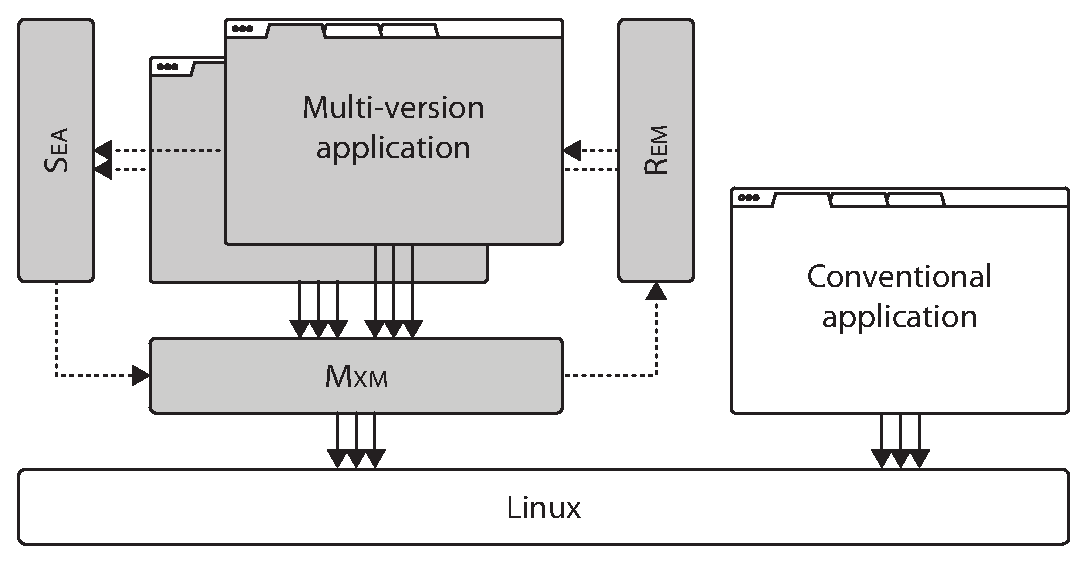
\includegraphics[width=0.6\columnwidth]{safe-updates/figures/architecture}
\caption{\mx system architecture.  
%% The main components of \mx
%%   are \sea (Static Executable Analyser), \mxm (Multi-eXecution
%%   Monitor), and \rem (Runtime Execution Manipulator).
}
\label{fig:design}
\end{center}
\end{figure}


\subsection{System call interposition}
\label{sec:mxm}

One of the main components of our multi-version execution environment
is the \mxm monitor.  \mxm's main jobs are to run the two versions
concurrently, mediate their interaction with the outside world,
synchronise their executions, and detect any divergences in their
external behaviour. \mxm works by intercepting all system calls issued
by each application version, and manipulating them to ensure that the
two versions are executed in a synchronised fashion and act as one to
the outside world.

\mxm provides functionality similar to conventional virtual machine monitors.
Whenever the MV application is executed, the \mxm connects to the two
application versions running in parallel, intercepting their kernel system
calls.  \mxm ensures that the two versions act as one to the outside world by
mediating access to the underlying operating system to achieve complete
isolation of the running application from other application instances as well
as from the external environment, making sure the combined application versions
act as one to the outside world.  The environment controlled by the monitor
consists mainly of a restricted file system access, socket interceptors and
signal handlers.

\subsubsection{System call interception}

\mxm is implemented using the  \ptrace interface provided by the Linux
kernel.  This interface, often used for application debugging, allows
simple deployment (without any need for compile-time instrumentation)
and makes the monitor itself lightweight since it is running as a
regular unprivileged process.  \mxm is similar in operation to previous
monitors whose goal is to synchronise applications at the level of system
calls such as \orchestra~\cite{orchestra09}, PLR~\cite{shye2009} or
\tachyon~\cite{tachyon12}.

\mxm runs each version in a separate child process, intercepting all
their system calls.  When a system call is intercepted in one version,
\mxm waits until the other version also performs a system call.  With
a pair of system calls in hand (one executed by the old version, and
one by the new version), \mxm compares their types and arguments.  If
they differ, \mxm has detected a divergence and invokes the \rem
component to resolve it (\S\ref{sec:rem}).

Otherwise, if the two versions perform the same system call with the
same arguments, \mxm virtualises their interaction with the
environment.  If the operation performed by the system call has no
side effects and does not involve virtualised state (\eg
\lstinline`sysinfo`), \mxm allows both processes to execute it
independently.  Otherwise, it executes the system call on their
behalf and copies its results into the address spaces of both
versions.

\mxm must also enforce deterministic execution across versions. This
consists mainly of intercepting instructions that may produce
non-deterministic results, and returning the same result in both
versions.  Examples of such non-deterministic operations include
random number generators (\eg read calls to \lstinline`/dev/[u]random`),
date and time (\eg read calls to \lstinline`/etc/localtime`), and access
to files and network (\eg file descriptor consistency).  Note that
non-deterministic effects resulting from allocating memory objects at
different addresses in memory or randomly arranging memory areas via
address space layout randomisation (ASLR) do not pose any
problems: \mxm understands the semantics of individual system calls and
rather than directly comparing memory addresses (which might be
different in each executed version), it compares the actual values
stored at those memory locations. \mxm supports both memory buffers (by
comparing the actual buffer content) as well as data structures
referenced by pointers (including nested ones).
 
Since \mxm fully controls executing programs intercepting all their system
calls, it can ensure that both programs have the same view of their
environment. Whenever the monitored process makes a system call, \mxm is
notified twice---first before, then after the call has been executed.  When a
\ptrace event is raised (\eg a new child process has been started), the monitor
is notified as well.  Due to internal limitations of the \ptrace interface,
once the system call has been made, it cannot be skipped, so when \mxm wants to
execute the call on behalf of its child processes, it simply replaces it with a
system call that does not change the system state (\lstinline`getpid` in our
case).

There are several challenges that we encountered while implementing
\mxm.  First, \mxm must partly understand the semantics of 
system calls.  For example, many system call parameters use complex
(often nested) structures with complicated semantics to pass values to
the operating system kernel, as in the case of \lstinline`ioctl` or
\lstinline`futex`.  To be able to compare the parameters of
these system calls and copy back their results, \mxm needs to
understand the semantics of these structures.  However, there are only
a relatively small number of system calls in Linux, and once the support
for handling them is implemented, it can be reused across applications.
\mxm currently implements \syscallsImplemented system calls (out of the
\syscallsTotal provided by Linux x86-64 3.1.9), which was enough to
allow us to run \mx on our benchmarks
(\S\ref{sec:reliability-evaluation}).

Second, the arguments of a system call are often passed through pointers,
which are only valid in the application address space, which is not directly
available to \mxm.  Therefore, \mxm needs to copy the contents pointed to by
these structures to its own address space in order to perform their
comparison.  The \ptrace interface on x86-64 only allows to copy one quadword
per system call, which is very expensive. Previous approaches either used
various ad-hoc optimisations~\cite{orchestra09} such as named pipes or shared
memory with custom shellcode, or a modified kernel~\cite{tachyon12} to
overcome this limitation. Instead, \mxm uses \emph{cross memory attach}, a new
mechanism for fast interprocess communication which has been recently added to
the Linux kernel~\cite{crossmemoryattach}.  This mechanism provides two new
system calls---\lstinline`process_vm_readv` and
\lstinline`process_vm_writev`---which allows the tracer to directly access the
memory space of the tracee using an interface similar to the \lstinline`readv`
and \lstinline`writev` system calls without any additional overhead.

Third, because the structures passed as arguments to system calls often have
variable size, \mxm also needs a fast way to allocate and deallocate memory
for them in order to minimise the overall overhead imposed by our system.  For
this purpose, \mxm uses a region-based memory allocator~\cite{memory-pools},
namely the \textsf{obstack}
library,\footnote{\url{http://www.gnu.org/software/hello/manual/libc/Obstacks.html}}
which is part of the \gnu C Library.  Each monitored process has its own
region, which is used for allocating memory to store the copy of the process'
system call arguments

\subsubsection{Multi-process and multi-threaded applications}

Finally, a particular challenge arises in the context of multi-process and
multi-threaded applications.  Using a single monitor instance to intercept both
versions and their child processes (or threads) would eliminate any advantage
that these applications derive from using concurrency.  Therefore, \mxm uses a
new monitor thread for each set of child processes (or threads) spawned by the
application.  For instance, if the old and new versions each have a parent and
a child process, then \mxm will use two threads: one to monitor the parent
processes, and one to monitor the child processes in each version.

Due to limitations of the \ptrace interface (which was not designed to be used
in a multi-process or multi-threaded environment), handing the control of any
child processes being spawned by the application over to a new monitoring
thread is somewhat complicated.  In \mxm we adopt a solution similar to
Orchestra~\cite{orchestra09}.  When a new child process is spawned, we let the
parent monitoring thread to supervise its execution until the first system
call.  Then, we replace this system call with a \lstinline`pause` system call,
disconnect the parent monitor (which causes a \lstinline`SIGCONT` signal to be
sent to all new child processes), and spawn a new monitoring thread which
immediately reconnects to the new child process, restores its original system
call, and resumes its execution.

\mxm does not enforce deterministic execution across multiple versions of
multi-threaded programs (which may diverge if race conditions can lead
to different external behaviour across executions), although we could
overcome this limitation by adopting \varan's solution
(\S\ref{sec:threading}).

%% \mxm also performs a series of optimisations to decrease performance
%% overhead, such as allowing certain files with read-only permissions
%% to be opened directly by the process. 

\subsubsection{Environment virtualisation}

To improve I/O performance and decrease virtualisation overhead,
processes are allowed to open files with read-only permissions
directly, while files with write permissions are opened by the monitor
itself.  This imposes another problem as file descriptors assigned to
these files are not necessarily the same in each version (\eg due to
scheduling non-determinism). Therefore, \mxm needs to virtualise
these file descriptors.

Whenever the monitored process opens a file with read-only permissions, a
new virtual file descriptor is assigned to this file together with the
mapping to a real file descriptor for each version. This virtual file
descriptor is then sent to each version. When a system call is made
using this virtual file descriptor, \mxm replaces it with the real
file descriptor before executing the system call. The actual file
operation is then executed by the process itself avoiding any memory
copying by \mxm.

A similar approach is also used for virtualisation of process,
group, parent and child identifiers.  Whenever a process tries to obtain
the actual ID, \mxm replaces this with a virtual ID and keeps the
mapping between the real and the virtual ID. When a process invokes a
system call using this ID as an argument (\eg \lstinline`kill`), the
virtual ID is replaced with the actual ID before executing the system
call.

%% \paragraph{Para-virtualisation interface and binary translation.}
%% Furthermore, we plan to combine this API with a binary translation
%% approach~\cite{binary-translation}, that will allow to dynamically
%% replace certain system calls with more efficient \emph{monitor
%% call} instructions.  The binary translation could be also used to
%% dynamically replace code components that have been proved to be
%% safe and do not need to be replicated across multiple versions (\eg
%% using static verification during compilation, using traces of
%% previous execution, using runtime heuristics).


%% \paragraph{Future work}

%% The \texttt{ptrace} interface allows us to easily monitor the program
%% execution without any compile-time instrumentation.  The main downside
%% of this approach is a relatively high overhead.  This is especially
%% true for I/O intensive applications, as they require frequent
%% transfers of large portions of the application memory space to the
%% monitor process. This overhead could be eliminated by directly
%% accessing the process memory space.

%% The existing prototype implementation of \textsc{Mxm} already supports
%% simple scenarios. The main limitation of this implementation is the
%% strict ordering of system calls, which must be the same in each
%% monitored application version.  To be practically usable, future
%% versions of \textsc{Mxm} need to relax the requirement on strict
%% ordering to allow more complex scenarios. This is especially important
%% when executing different versions of the same application.

%% Most importantly, a straightforward comparison of system call traces
%% is usually not sufficient to identify divergences, since different
%% versions might use a slightly different sequence of kernel and library
%% calls to implement the same behaviour.  We plan to explore approaches
%% similar to those implemented by compiler optimisations, such as
%% \emph{peep-hole optimisation}~\cite{dragon-book}, and adapt them to
%% work on the level of kernel and library calls.


%% %% \paragraph{Hashing system call traces.}
%% %% To decrease the overhead of kernel and library call synchronisation, we aim to
%% %% enhance our system to hash the sequence of system call traces using fast hash
%% %% functions such as FNV-1 or FNV-1a.  This approach has a significant advantage
%% %% over straightforward comparison of call traces, especially in the case of
%% %% system calls with virtually unlimited parameter sizes such as \texttt{read} or
%% %% \texttt{write}~\cite{shye2009}.  Similar approach has been already used
%% %% in~\cite{shye2009}.

%% \paragraph{Libraries support and virtualisation.}
%% Since many applications today use functionality provided by shared
%% libraries, we aim to support intercepting calls to such libraries as
%% well. Moreover, as intercepted calls to shared libraries can be
%% executed only once, same as in the case of system call monitoring,
%% this may decrease the overall overhead of multi-version execution.

%% We also plan to provide our own implementation of the \texttt{libc}
%% library loaded using the \texttt{LD\_PRELOAD} mechanism.  This library
%% will communicate directly with the monitor process through shared
%% memory, decreasing the number of system calls that need to be directly
%% intercepted, and thus resulting in much better performance.  However,
%% since the \texttt{LD\_PRELOAD} mechanism can be overridden, we still
%% need to combine it with the \texttt{ptrace} monitoring facility to
%% achieve complete isolation with reasonable overhead.  This approach
%% can be extended to support other shared libraries as well, further
%% improving the overall performance of our approach.

\subsection{Runtime state manipulation}
\label{sec:rem}

At the core of our system lies the \rem component, which is invoked
by \mxm whenever a divergence is detected.  \rem has two main jobs:
(1)~to decide whether to resolve the divergence in favour of the old or
the new version; and (2)~to allow the other version to execute through
the divergence and resynchronise the execution of the two versions
after the divergence.
%% The first task by itself it's easy: we favour the new version, except
%% for when it crashes.
%% As discussed in \sref{sec:scope}, in this paper we restrict our
%% attention to surviving crash errors, so the first task is relatively
%% easy: if one of the two versions crashes, we use the output of the
%% other version; otherwise, we always favour the new version.  
%%
%% The second task is however more difficult, but essential to the
%% success of our approach, which relies on having both versions be alive
%% at all times, so that the overall application can survive any crash
%% bugs that happen in either the old or the new version (although of
%% course, not in both).
%%
As discussed in Section~\ref{multi-version:rationale}, in \mx we focus
our attention on surviving crash errors, so the key challenge is to
allow the crashing version to survive the crash.  This is essential to
the success of our approach, which relies on having both versions alive
at all times, so that the overall application can survive any crash bugs
that happen in either the old or the new version (although of course,
not in both at the same time).

We emphasise that we apply our approach only to crash errors (those
raising a \lstinline`SIGSEGV` signal), and not to other types of program
termination, such as \lstinline`abort`.  This is important from a
security perspective, because
%% many patches turn potential compromises into
%% run-time {\small{\texttt{abort}s}}, \eg using assertions for input
%% sanitisation.  For example, 
when a vulnerability is discovered, but a proper solution is not yet
known, developers often\footnote{For example, see the patch in \texttt{json-cpp}~\url{http://jsoncpp.svn.sourceforge.net/viewvc/jsoncpp/trunk/jsoncpp/include/json/assertions.h?r1=247&r2=246&pathrev=247}}
fail-stop the program rather than letting it continue and allowing
the attacker to compromise the system.
%
%% Such situations can be easily distinguished since failed assertions
%% result in program abortion (\ie
%% \textstt{SIGABRT} signal), while unintentional program crashes typically
%% result in abnormal termination (\ie \textstt{SIGSEGV} signal). 
%% Therefore, \rem only intercepts and handles crashes resulting
%%   in \textstt{SIGSEGV} signals.

Suppose that one of the versions has crashed between the execution of
system call $s_1$ and the execution of system call $s_2$.  Then, in
many common scenarios, the code executed between the two system calls
is responsible for the crash (\eg the old version crashes because it
doesn't incorporate a bug fix present in the new version, or the new
version crashes because its code was patched incorrectly).  Therefore,
our strategy is to do a form of \textit{runtime code patching}, in
which we use the code of the non-crashing version to execute over the
buggy code in the crashing version.

%% If the behaviour of the two versions is different, but they both
%% continue to execute, then we favour the behaviour of the new version and
%% wait for the two versions to reconverge.

%% There are many different ways to achieve this goal, such as the use of
%% a mechanism based on check-pointing and roll-back~\cite{qin2005};
%% however, these mechanisms cannot deal with persistent errors which are
%% common in the case of software updates.

%% Our solution is based upon the observation that errors in programs are
%% usually located at particular places (\ie specific instructions) in
%% the program's code.  Therefore, we can use the code of the other, and
%% \ie correct, version to execute over this critical point in program's
%% code. This approach may not work when memory layout of the two
%% versions differs, as the code of one version may fail to locate the
%% memory structures necessary for its execution in the memory of the
%% other version. Nevertheless, the described approach might still work
%% in many cases when memory layout of the two versions does not differ
%% significantly.


%\paragraph{Possible execution scenarios.}

%% We run two versions of the same application in parallel, monitoring
%% their execution to be sure that they behave in the same way without
%% any divergences by comparing the application executions at
%% synchronisation points; in case of our prototype equal to system
%% calls. When either of the versions fail, we stop its execution at the
%% \emph{divergence point}; at this point there are three possible
%% solutions to synchronise the divergent versions:

\begin{figure}[t]
\centering
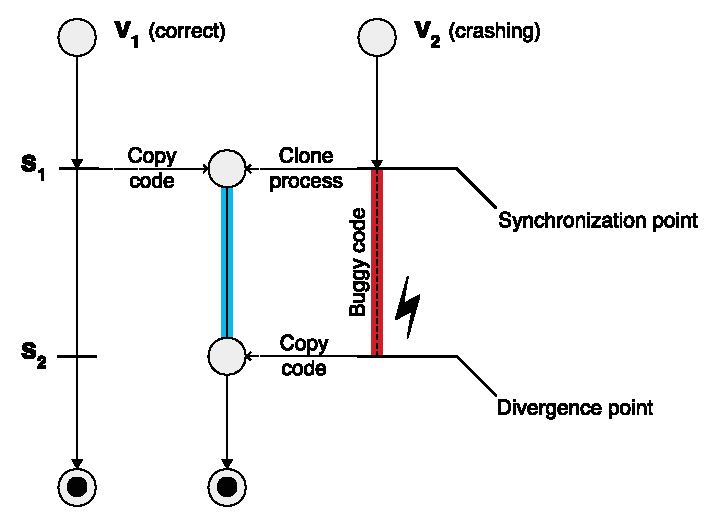
\includegraphics[width=0.5\columnwidth]{safe-updates/figures/strategy}
\caption{\rem's recovery mechanism uses the code of the non-crashing
  version to run through the buggy code.}
\label{fig:solution3}
\end{figure}

%% \begin{enumerate}[label=\emph{S\arabic*}, itemsep=3pt, parsep=3pt]
%% \renewcommand*\labelitemi{\emph{S\arabic*}}
%% \begin{figure}[t]
%%   \centering
%%   \subfloat[Patch state after the crash and continue execution]{
%%     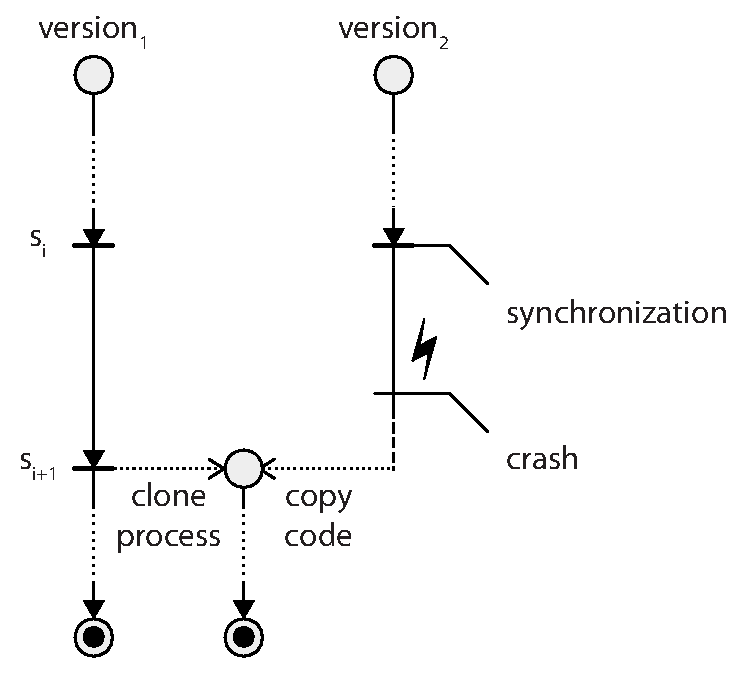
\includegraphics[width=0.45\columnwidth]{safe-updates/figures/solution1}
%%     \label{fig:solution1}
%%   }
%%   \quad
%%   \subfloat[Patch state before the crash and continue execution]{
%%     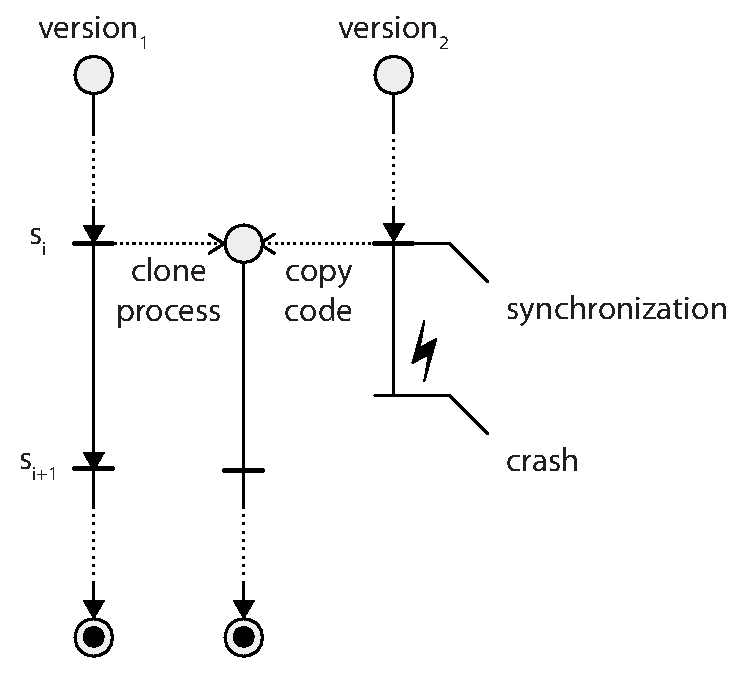
\includegraphics[width=0.45\columnwidth]{safe-updates/figures/solution2}
%%     \label{fig:solution2}
%%   }
%%   \\
%%   \subfloat[Use the code of older version only to run through critical section]{
%%     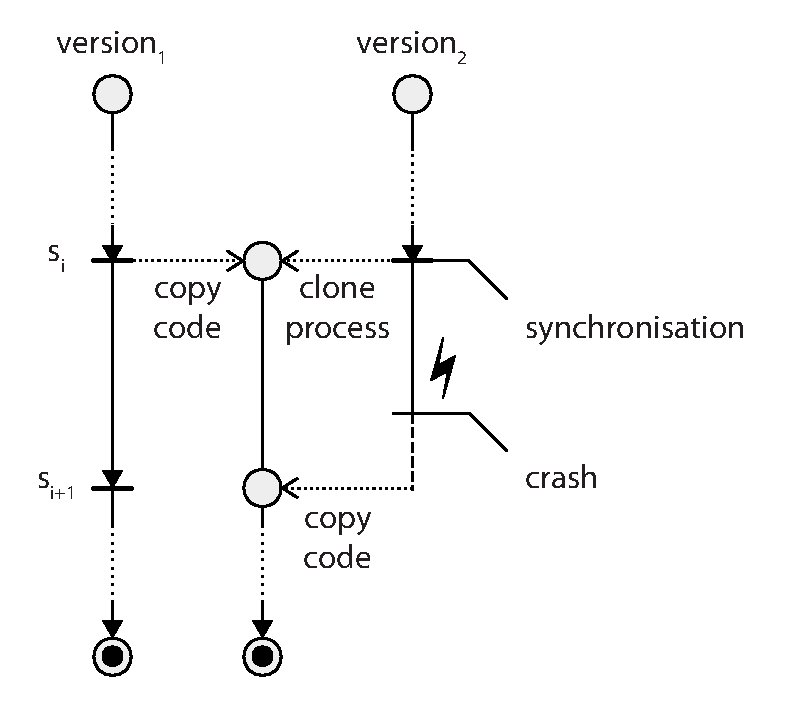
\includegraphics[width=0.45\columnwidth]{safe-updates/figures/solution3}
%%     \label{fig:solution3}
%%   }
%%   \caption{Three solutions for synchronising two divergent versions of
%%   the same application}
%%   \label{fig:solution}
%% \end{figure}

%% \item\label{s1} Clone the correctly executing version to duplicate its state
%%   (\eg memory content, memory mappings) after the crash and replace its
%%   code with the code of the failed version. Then restart both versions and
%%   continue their execution (Figure~\ref{fig:solution1}).

%% \item\label{s2} Clone the correctly executing version to duplicate its state
%%   (\eg memory content, memory mappings) at the last synchronisation point (\ie
%%   creating checkpoint). After the crash, replace the code of this cloned
%%   version with the code of the failed version. Then restart this cloned
%%   version, execute over the \emph{critical section}, and continue execution of
%%   both versions (Figure~\ref{fig:solution2}).

%% \item\label{s3} Clone the failing version to duplicate its state (\eg memory
%%   content, memory mappings) at the last synchronisation point (\ie creating
%%   checkpoint). After the crash, replace the code of this cloned version with
%%   the code of the correctly executing version. Then restart this cloned
%%   version; after the application successfully executes over the \emph{critical
%%   section}, replace the code of the cloned version again with the original
%%   code, and continue its execution (Figure~\ref{fig:solution3}).

%% \end{enumerate}

Our exact recovery mechanism is illustrated in
Figure~\ref{fig:solution3}.  At each system call, \mx creates a
lightweight checkpoint of each version.  This is implemented using the
\lstinline`clone` system call in Linux, which internally uses a
copy-on-write strategy.  
%% As an important optimisation, we omit system
%% calls that can be replayed safely from the last checkpoint, such
%% as \textstt{read}.

As shown in Figure~\ref{fig:solution3}, suppose that the crash happens in
version $v_2$, between system calls $s_1$ and $s_2$.  Then, \rem first restores
$v_2$ at point $s_1$ (\circl{A}), copies $v_1$'s code into $v_2$'s code segment
(\circl{B}), executes over the buggy code using $v_1$'s code (\circl{C}, note
that we are still using $v_2$'s memory state), and then restore $v_2$'s code at
point $s_2$ (\circl{D}).

There are several challenges in implementing this functionality.
First, \rem needs the ability to read and write the application's code
segment.  In the current implementation, we bypass this by linking
together the two application versions after renaming all the symbols
in one of the versions using a modified version of
the \texttt{objcopy}
tool.\footnote{\url{http://sourceware.org/binutils/docs/binutils/objcopy.html}}
However, in the future we plan to implement this transparently by
using the cross-memory attach mechanism used by \mxm.
%% \textstt{pread} and \textstt{pwrite} interface to directly
%% read and write the process memory via the
%% %\textstt{/proc/<pid>/mem} file in the
%% \emph{proc} file system.

%% This functionality has been recently introduced to the Linux kernel in
%% version 2.6.39~\cite{kernel-procmem}; previously, this interface was
%% read-only. This approach imposes only minimal overhead as it allows
%% direct access to the process memory space.

%% The runtime process manipulation functionality is implemented inside
%% \rem, a separate component used by the \mxm monitor. The
%% manipulation itself is driven by the data obtained statically by the
%% \sea analyser before the application has been executed.

Second, \rem needs to modify the contents of the stack in $v_2$.  This is
necessary because the return addresses on the stack frames of $v_2$ still point
to $v_2$'s original code, which was now replaced by $v_1$'s code.  Without also
modifying $v_2$'s stack, any function
\lstinline[language={[x64]Assembler}]`RET` instruction executed between $s_1$
and $s_2$ would most likely veer execution to an incorrect location, since
function addresses are likely to be different across different versions.  Thus,
after \rem replaces $v_2$'s code, it also updates the return addresses on
$v_2$'s stack with the corresponding return addresses in $v_1$, which are
obtained via static analysis (\S\ref{sec:sea}).  Because system calls are
invoked via wrapper functions in C library, this ensures that when $v_2$
resumes execution, it will immediately return to the code in $v_1$.
%% \rem obtains these addresses by analysing $v_1$'s stack at
%% position $s_1$ accessible via checkpoint taken at that point.
%
To implement this functionality, \rem makes use of
the \texttt{libunwind}
library,\footnote{\url{http://www.nongnu.org/libunwind/}} which provides a
portable interface for accessing the program stack, for both x86 and
x86-64 architectures. To actually modify the execution stack of
$v_2$, \rem uses again the \ptrace interface.


Unfortunately, updating the stack return addresses is not sufficient
to ensure that $v_2$ uses $v_1$'s code between $s_1$ and $s_2$, as
$v_2$ may also use function pointers to make function calls.
%% Note that we are still using the $v_2$ memory state. Thereby, $v_2$
%% may still issue a function call to the original code through one of
%% the function pointers.
To handle such cases, \rem inserts breakpoints to the first
instruction of every function in $v_2$'s original code.  Then, when a
breakpoint is encountered, \rem is notified via a \lstinline`SIGTRAP`
signal, and redirects execution to the equivalent function in $v_1$'s
code (which is obtained from the \sea component) by simply changing
the instruction pointer.
%The address of the equivalent function is obtained

Finally, after executing through the buggy code, \rem performs the
same operations in reverse: it redirects execution to $v_2$'s original
code, changes the return addresses on the stack to point to $v_2$'s
functions, and disables all breakpoints inserted in $v_2$'s code.  
The one additional operation that is done at this point is to copy all
the global data modified by $v_1$'s code into the corresponding
locations referenced by $v_2$'s code.  

%\paragraph{Runtime stack analysis and manipulation.}

%% For example, on the x86 architecture, the stack can be easily
%% traversed starting from the top as each stack frame contains frame
%% pointer pointing to the previous stack frame, thereby forming a linked
%% list-like structure. This is not possible on the x86-64 architecture
%% as the frame pointer is no longer stored inside the stack frame.  To
%% traverse the execution stack on this architecture, it is necessary to
%% compute sizes of all functions' stack frames using the stack usage
%% information stored in the \texttt{UNWIND\_CODE} section, which is a
%% part of the ELF binary file. This logic is implemented by the
%% \texttt{libunwind} library, which provides API to unwind the stack
%% independent of the target platform.

%The necessary information about the stack location (\ie address range) and
%page mapping are obtained through the \emph{proc} file system; in particular
%the \textstt{/proc/<pid>/maps} and \textstt{/proc/<pid>/pagemap} files.

Note that \mx cannot currently handle major modifications to the
layout of the data structures used by the code, including individual
stack frames.  While this still allows us to support several common
software update scenarios, in future work we plan to improve the
system with the ability to perform full stack
reconstruction~\cite{upstare} and automatically infer basic data
structure changes at the binary-level~\cite{data-struct-digging}.
%% to identify changes to function names and sequences of function calls
%% (e.g., via clone detection techniques~\cite{cp-miner06,deckard07}),


Our approach of using the code of the non-crashing version to survive failures
in the crashing version may potentially leave the recovered version in an
inconsistent state. However, \mx is able to discover most internal state
inconsistencies by checking whether the two versions have the same external
behaviour after recovery. When the behaviour of the recovered version starts to
differ, \mx will immediately discard it and continue with only one version. The
discarded version can be later restarted at a convenient synchronisation point.
This restarting functionality is not currently implemented in \mx, but we plan
to add it as a future extension.

%Our approach of using the code of the non-crashing version to survive
%failures in the crashing one may leave the application in an
%inconsistent state, and thus may not be applicable for application in
%which absolute correctness and a fail-fast approach are more important
%than allowing the application to survive errors.  However, \mx is
%usually able to discover most internal state inconsistencies, since it
%regularly checks if the two versions have the same external
%behaviour. (See \S\ref{sec:discussion} for an extended discussion.)

\subsection{Binary static analysis}
\label{sec:sea}

%% \begin{table*}[t]
%% \centering 
%% \begin{tabular}{ccc}
%%   \hline
%%   Library calls in $\mathrm{version}_1$ & Library calls in $\mathrm{version}_2$ &
%%   System calls within the library \\
%%   \hline
%%   \texttt{<0xdeadbe5a>} & \texttt{<0xdeadbe8e>} &
%%   [\texttt{<0x77ff2c>}, \texttt{<0x77ffae>}] \\
%%   \texttt{<0xdeadabf5>} & \texttt{<0xdeadac34>} &
%%   [\texttt{<0x782bae>}] \\
%%   \vdots & \vdots & \vdots \\
%% \end{tabular}
%% \caption{Addresses of library function calls, and system calls invoked from
%% within these functions.}
%% \label{tab:syscall_table}
%% \end{table*}

The \sea component statically analyses the binaries of the two
versions to obtain information needed at runtime by the \rem
component.  \sea is invoked only once, when the multi-version
application is assembled from its component versions.
%% As mentioned in \sref{sec:rem}, we currently link together the
%% two application versions after renaming all the symbols in one of them
%% using a modified copy of the \textstt{objcopy} tool, although in the
%% future we plan to do this linking dynamically by directly changing the
%% code segment in each version.

The main goal of \sea is to create several mappings from the code of
one version to the code of the other.  First, \sea extracts the
addresses of all function symbols
in one version and maps them to the
addresses of the corresponding functions in the other version.  This
mapping is used by \rem to handle calls performed via function
pointers (\S\ref{sec:rem}).

Second, \sea computes a mapping from all possible return addresses in
one version to the corresponding return addresses in the other version.  In
order to allow for code changes, this mapping is done by computing an
ordered list of all possible return addresses in each function.  For
example, if function \lstinline`foo` in $v_1$ performs call instructions
at addresses \lstinline`0xabcd0000` and \lstinline`0xabcd0100`, and
function \lstinline`foo` in $v_2$ performs call instructions at
addresses \lstinline`0xdcba0000` and \lstinline`0xdcba0400`, then \sea
will compute the mapping \texttt{\{0xabcd0005 $\rightarrow$
0xdcba0005, 0xabcd0105 $\rightarrow$ 0xdcba0405\}} (assuming each call
instruction takes 5 bytes).  This mapping is then used by \rem to
rewrite return addresses on the stack.

%% These data are gathered by the \sea analyser component which
%% implements static analysis of binary executables to extract all
%% necessary addresses and provide them to other components inside our
%% system. The format used for storing these data is represented by a
%% \emph{call table}. For each version, this table contains addresses of
%% all calls to shared library functions together with the list of all
%% system calls addresses invoked within these library functions, as can
%% be seen in Table~\ref{tab:syscall_table}.

%% For example, the first line of this table represents a call to a
%% library function which does two system calls, while second line
%% represents a function call which does only one system call.

To construct these tables, \sea first needs to extract the addresses
of all function symbols and then disassemble the code for each
individual function in order to locate the call instructions within
them.  The implementation is based on the \texttt{libbfd}
and \texttt{libopcodes} libraries, which are 
part of the
\gnu \binutils suite.\footnote{\url{http://www.gnu.org/software/binutils/}}
To obtain the addresses of all function symbols defined by the
program, \sea uses \texttt{libbfd} to extract the static and dynamic
symbol tables and relocation tables.  To disassemble individual
functions, \sea uses the \texttt{libbf}
library~\cite{kwan:libbf}, built on top of \texttt{libopcodes}.

%% Disassembled machine code is stored in a graph-like structure where
%% individual instructions represents vertices and edges between these
%% vertices represents the control flow. 

%% \paragraph{System call identification.}
%% \sea implementation uses the disassembler to obtain machine
%% code of each individual function and iterates over its instructions
%% (traversing the instruction graph) to identify basic blocks and locate
%% system call instructions within the code these functions.

%% To locate system calls within shared library function calls,
%% \sea first needs to obtain the set of exported library
%% functions and system calls within these functions using the above
%% described approach. Then, \sea analyses the application binary
%% itself and locates all function calls to the shared library using the
%% information extracted from relocation and procedure lookup tables
%% contained in ELF binaries.

%% Results of this analysis are stored in a hash table and tree structure
%% to allow quick access eliminating any unnecessary overhead when these
%% information are accessed during runtime. These data are then used to
%% construct the already described \emph{call table}, before the
%% application itself is executed.

%% \subsection{Limitations and Future Work}
%% \label{sec:limitations}
%% \input{limitations}


%\section{Evaluation}
%\label{sec:evaluation}
%\section{Reliability Evaluation}
\label{sec:reliability-evaluation}

To evaluate our approach, we show that \mx can survive crash bugs in several
real applications (\S\ref{sec:surviving}). We then examine the question of how
far apart can be the versions run by \mx (\S\ref{sec:bounds}), and discuss
\mx's performance overhead (\S\ref{sec:performance}).

\subsection{Fault recovery}
\label{sec:surviving}

We have evaluated \mx using a set of bugs in three applications: \gnu
\coreutils, \redis and \lighttpd. We discuss each application in turn below.

\subsubsection{\gnu \coreutils}
\label{sec:coreutils}

\begin{table}[t]
\begin{center}
\caption{Utilities from \gnu \coreutils, the crash bugs used, and the 
versions in which these bugs were introduced and fixed.  We group
together utilities affected by the same or similar bugs.}
\begin{tabular}{lll}
\toprule
\textsc{Utility} & \textsc{Bug description} & \textsc{Bug span} \\
\midrule
\mdsum & \multirow{2}{*}{Buffer underflow} & \multirow{2}{*}{v5.1 -- v6.11} \\
\shasum & & \\
\midrule
\mkdir & \multirow{2}{*}{\textstt{NULL}-pointer dereference} & \multirow{2}{*}{v5.1 -- v6.11} \\
\mkfifo & & \\
\mknod & & \\
\midrule
\cut & Buffer overflow & v5.3 -- v8.11 \\
\bottomrule
\end{tabular}
\label{tbl:cu-bugs}
\end{center}
\end{table}

As an initial evaluation of \mx's ability to survive crashes, we have used
applications from the \gnu \coreutils utility
suite,\footnote{\url{http://www.gnu.org/software/coreutils/}} which provides
the core user-level environment on most UNIX systems.  We have selected a
number of bugs reported on the \coreutils mailing list, all of which trigger
segmentation faults.  The bugs are described in Table~\ref{tbl:cu-bugs},
together with the utilities affected by each bug and the versions in which they
were introduced and fixed.

The bug affecting both \mdsum and \shasum utilities introduced in 5.1 and later
fixed in 6.11 caused a crash due to buffer underflow when checking an invalid
BSD-style input. Another bug we have considered affected \mkdir, \mkfifo and
\mknod utilities; this bug, which was reported in 6.10 and fixed in 6.11
resulted in crash when diagnosing invalid context.  Finally, the bug affecting
\cut utility, introduced in 5.3 and later fixed in 8.11, resulted in segfault
when using large unbounded range. 

For all these bugs, we configured \mx to run the version that fixed the bug
together with the one just before.  (we could have also run the version that
introduced the bug with the one just before, but we could not immediately tell
where the bug was introduced, and we cannot build versions earlier than 6.10
due to changes in GCC and GNU C library).  \mx successfully intercepted the
crash and recovered the execution by using the strategy described in
\sref{sec:rem}.

We discuss below the bug in the \cut utility (used to remove sections from each
line of file), triggered by the following invocation:

\begin{lstlisting}[numbers=none,breaklines=true,xleftmargin=0pt,language=bash]
cut -c1234567890- --output-d=: foo
\end{lstlisting}

This bug is triggered by the conditional statement on line~\ref{line:cond}:

\begin{lstlisting}[firstnumber=525]
if (output_delimiter_specified /*@\label{line:cond}@*/
    && !complement
    && eol_range_start && !is_printable_field (rsi_candidate))
\end{lstlisting}

This code uses the lower bound of the size of the printable field
vector; however, when calculating the size of this vector, ranges going
to the end of line (\ie \lstinline`0-`) are not considered eventually
resulting in invalid memory access. 
% The bug is caused by a buffer overflow whose root cause is the
% incorrect calculation of the size of a dynamically allocated buffer
% used internally by \cut.
When \mx intercepts this bug, it uses the
last checkpoint to recover the execution of the crashing version. This
checkpoint is taken after the \textstt{brk} system call triggered by
the \textstt{malloc} call that allocates the buffer. 
% in function \textstt{bindtextdomain} on line~\ref{line:bind}.
% \begin{lstlisting}[firstnumber=767]
% bindtextdomain (PACKAGE, LOCALEDIR); /*@\label{line:bind}@*/
% \end{lstlisting}
The recovered process uses the code of the other version to correctly
calculate the size of the field vector and switches back to the original
code during the allocation of this buffer as
%code during the allocation of this buffer on line~\ref{line:alloc} as
function \textstt{xzalloc} triggers \textstt{mmap64} system call, just
before executing the conditional statement on line~\ref{line:cond},
which originally triggered the bug.

\subsubsection{\redis}
\label{sec:redis}

Below, we describe how \mx can survive the \redis bug described in
Section~\ref{multi-version:scenarios} while running in parallel the \redis
revision \textstt{a71f072f} (\textit{the old version}, just before the bug was
introduced) with revision \textstt{7fb16bac} (\textit{the new version}, just
after the bug).  \mx first invokes \sea to perform a static analysis of the two
binaries and construct the mappings described in \sref{sec:sea}.  Then, \mx
invokes the \mxm monitor, which executes both versions as child processes and
intercepts their system calls.

When the new version crashes after issuing the problematic
\textstt{HMGET} command, \mxm intercepts the \textstt{SIGSEGV} signal
which is sent to the application by the operating system.  At
this point, \rem starts the recovery procedure.  First, \rem sends a
\textstt{SIGKILL} signal to the new version to terminate it.  It then
takes the last checkpoint of the new version, which was taken at the
point of the last invoked system call, which in this case is an
\textstt{epoll\_ctl} system call.  Then, \rem uses the information
provided by \sea to rewrite the stack of the new version, as detailed
in \sref{sec:rem}.  In particular, \rem replaces the return
addresses of all functions in the new version with the corresponding
addresses from the old version. The stack rewriting itself however is not
enough. The newer version can still use function pointers, which are part of
the replica state, to invoke the original code. To prevent this situation, \rem
inserts breakpoints at the beginning of all the functions in the code of the
new version (to intercept indirect calls via function pointers), and then
finally restores the original processor registers of the checkpointed process
and restarts the execution of the (modified) new version.

Since the checkpoint was performed right after the execution of the system
call \textstt{epoll\_ctl}, the first thing that the code does is to
return from the \textstt{libc} wrapper that performed this system
call.  This in turn will return to the corresponding code in the old
version that invoked the wrapper, since all return addresses on the
stack have been rewritten.  From then on, the code of the old version
is executed (but in the state of the new version), until the first
system call is intercepted.  In our example, the old and the new
versions perform the same system call (and with the same arguments),
so \rem concludes that the two processes have re-converged, and thus
restores back the code of the new version by performing the steps
above in reverse, plus the additional step of synchronising their
global state (see \S\ref{sec:rem}).  Finally, the control is handed
back to the \mxm monitor, which continues to monitor the execution of
the two versions.

\subsubsection{\lighttpd}
\label{sec:lighttpd}

To evaluate \mx on \lighttpd, we have used two different crash bugs.
The first bug is the one described in detail in
Section \ref{multi-version:scenarios}, related to the ETag and compression
functionalities.  As previously discussed, the crash is triggered by a
very small change, which decrements the upper bound of a \textstt{for}
loop by one.  \mx successfully protects the application against this
crash, and allows the new version to survive it by using the code of
the old version.

The other crash bug we reproduced affects the URL rewrite
functionality.\footnote{\url{http://redmine.lighttpd.net/projects/lighttpd/issues/2140}}
This is also caused by an incorrect bound in a \lstinline`for` loop.
More precisely, the loop: 

\begin{lstlisting}[numbers=none,breaklines=true,xleftmargin=0pt]
for (k=0; k < pattern_len; k++)
\end{lstlisting}

\noindent should have been:

\begin{lstlisting}[numbers=none,breaklines=true,xleftmargin=0pt]
for (k=0; k@+1@ < pattern_len; k++)
\end{lstlisting}

The bug seems to have been present since the very first version
added to the repository.  It was reported in December 2009, and
fixed one month later.  As a result, we are running \mx using the last
version containing the bug together with the one that fixed it.  While
this bug does not fit within the pattern targeted by \mx (where a
newer revision introduces the bug), from a technical perspective it is
equally challenging.  \mx is able to successfully run the two versions
in parallel, and help the old version survive the crash bug.

%The bug \#1601 affects the HTTP redirection functionality, in particular
%the \texttt{\%n} substitution with condition substring. This functionality has
%been introduced in revision \texttt{510}. However, there is an incorrect
%comparison in one of the conditions which causes segmentation fault when
%appending matched parts to buffer if there was no matching regular expression.
%The affected code can be seen in Listing~\ref{lst:510}.

%\begin{lstlisting}[label=lst:510, caption={Original correct version of the function}]
%cond_cache_t *cache = &con->cond_cache[dc->context_ndx];
%if (n > cache->patterncount) {
  %return 0;
%}
%\end{lstlisting}

%The fix to this bug consists of a single changed line as can be seen in
%Listing~\ref{lst:2138} and has been incorporated in revision \texttt{2138}, yet
%this bug remained undetected for nearly three years (August 8, 2005 --- March
%26, 2008) rendering \lighttpd webserver vulnerable to attack.

%\begin{lstlisting}[label=lst:2138, caption={Refactored failing version of the function}]
%cond_cache_t *cache = &con->cond_cache[dc->context_ndx];
%if (n >= cache->patterncount) {
  %return 0;
%}
%\end{lstlisting}

Both \lighttpd bugs \#1601 and \#2140 are very simple---their fix
consist of a single character---yet still they made \lighttpd server
vulnerable to a potential attack. \mx can not only handle the crash,
but also successfully recover the failing version in both cases.

\subsection{Ability to run distant versions}
\label{sec:bounds}

\begin{table}
\begin{center}
\caption{The maximum distance in number of revisions, and the time span
  between the revisions that can be run by \mx for each bug.}
\begin{tabular}{lcc}
\toprule
\textsc{Application Bug} & \textsc{Max distance} & \textsc{Time span} \\
\midrule
\lighttpd \#2169   & \maxDistLighttpdOne & \timeSpanLighttpdOne \\
\lighttpd \#2140   & \maxDistLighttpdTwo & \timeSpanLighttpdTwo \\
\redis \#344       & \maxDistRedis & \timeSpanRedis \\
%md5sum          & \maxDistMdsum & \timeSpanMdsum \\ \hline
\bottomrule
\end{tabular}
\label{tbl:bug-bounds}
\end{center}
\end{table}

In the previous sections, we have shown how \mx can help software
survive crash bugs, by running two \textit{consecutive} versions of an
application, one which suffers from the bug, and one which does not.
%
One important question is how far apart can be the versions run
by \mx.  To answer this question, we determined for each of the bugs
discussed above the most distant revisions that can be run together to
survive the bug.  

For the \coreutils benchmarks, we are able to run versions which are
hundreds of revisions apart: \maxDistMdsum~revisions (corresponding to
\timeSpanMdsum of development time) for the \mdsum/\shasum bug; 
\maxDistMkdir~revisions (\timeSpanMkdir of development time) for the 
\mkdir/\mkfifo/\mknod bug; and \maxDistCut~revisions (\timeSpanCut 
of development time) for the \cut bug.

The most distant versions for the first \lighttpd bug are
approximately two months apart and have \maxDistLighttpdOne~revisions
in-between, while the most distant versions for the second
\lighttpd bug are also approximately two months apart but have only
\maxDistLighttpdTwo~revisions in-between.  Finally, the most distant
versions for the \redis bug are \maxDistRedis~revisions
and \timeSpanRedis apart.  

Of course, it is difficult to draw any general conclusions from only
this small number of data points.  Instead, we focus on understanding
the reasons why \mx could not run farther apart versions for the bugs
in \lighttpd and \redis (we ignore \coreutils, for which we can run
very distant versions).
%% For the \coreutils bugs, the lower bound is the earliest
%% version that we could build and run on our machine (v6.10).  The
%% upper-bound for 
%
For \lighttpd issue \#2169, the lower bound is defined by a revision
in which a pair of \textstt{geteuid()} and \textstt{getegid()} calls
are replaced with a single call to \textstt{issetugid()} to
allow \lighttpd to start for a non-root user with GID~0.  \mx 
%cannot run this revision together with the one before it, because it 
currently does not support changes to the order of system calls, but we believe
this limitation could be overcome by using peephole-style
optimisations~\cite{dragon-book}, which would allow \mx to recognise
that the pair \textstt{geteuid()} and \textstt{getegid()} could be
matched with the call to \textstt{issetugid()}.  The upper bound
for \lighttpd issue \#2169 adds a \textstt{read} call to
\textstt{/dev/[u]random}, in order to provide a better entropy
source for generating HTTP cookies.  This additional \textstt{read}
call changed the sequence of system calls, which \mx cannot
handle. \looseness=-1

For \lighttpd issue \#2140, both the lower and the upper bounds are
caused by a change in a sequence of \textstt{read()} system calls.  We
believe this could be optimised by allowing \mx to recognise when two
sequences of read system calls are used to perform the same overall
read.

%% Lower bound: the fix consists of request parser changes which resulted
%% in different sequence of \textstt{read()} system calls. The different
%% sequence of \textstt{read()} calls also marked the upper bound in this
%% case, defined by revision \lighttpdTwoUB. In this revision, the way in
%% which input connection buffer is being filled has changed, fixing
%% issue \#2147 and CVE-2010-0295 vulnerability.

For the \redis bug, the lower bound is given by the revision in which the
\textstt{HMGET} command was first implemented.  Since there was no support for
\textstt{HMGET} before that version, \mx has no way to survive the crash caused
by invoking \textstt{HMGET} with a wrong type (see \S\ref{sec:redis}).  The
upper bound is defined by a revision which changes the way error responses are
being constructed and reported, which results in a very different sequence of
system calls.

%% , including the call on line
%% \ref{line:report-error2} in Listing~\ref{lst:refactored}, resulting in
%% different sequence of system calls.

%% \todo{explain that all of these changes are minor and some of them could be
%% very well handled by using window-based/peep-hole approach}

\subsection{Performance Overhead}
\label{sec:performance}

\begin{figure}[!t]
\centering
\includegraphics[width=\textwidth]{safe-updates/graphs/spec2006}
\caption{Normalised execution times for the \spec benchmark suite running under
\mx.}
\label{fig:spec}
\end{figure}

We ran our experiments on a four-core server with 3.50~GHz Intel
Xeon E3-1280 and 16~GB of RAM running 64-bit Linux v3.1.9.

\paragraph{\spec.}
To measure the performance overhead of our prototype, we first used
the standard \spec\footnote{\url{http://www.spec.org/cpu2006/}}
benchmark suite.  Figure~\ref{fig:spec} shows the performance of \mx
running two instances of the same application in parallel, compared to
a native system. The execution time overhead of \mx varies
from \minOverSPEC to \maxOverSPEC compared to executing just a single
version, with the geometric mean across all \numSPECbench benchmarks at
\avgOverSPEC. This result is comparable with previous work using multi-variant
execution that used SPEC CPU to measure performance~\cite{orchestra09} (even
though this work used SPEC~CPU2000 which has already been retired).

%% The overhead varies from \minRedisOver to \maxRedisOver depending
%% on the operation being performed. This is the worst case overhead
%% we have seen among all tested application and comes mainly from the
%% fact that \redis is an in-memory database optimised for maximum
%% bare-hardware performance and is very sensitive to any additional
%% software layers.  Even a state-of-the-art hypervisor can incur an
%% $n$-fold slowdown, so the relatively high measure overhead is
%% therefore unsurprising.

\paragraph{\gnu~\coreutils.} The six \coreutils applications discussed in 
\sref{sec:coreutils} are mostly used in an interactive fashion via the
command-line interface (CLI). For such applications, a high performance
overhead is acceptable as long as it is not perceptible to the user;
prior studies have shown that response times of less than 100ms
typically feel instantaneous~\cite{card:human_proc}. In many common use
cases (\eg creating a directory, or using \cut on a small text file),
the overhead of \mx was imperceptible---\eg creating a directory takes
around \avgMkdirNative natively and \avgMkdirMx with \mx. For the three
utilities that process files, we calculated the maximum file size for
which the response time with \mx stays under the 100ms threshold.  For
\cut, the maximum file size is \cutCutoffSize (with an overhead of
\cutCutoffOver), for \mdsum \mdsumCutoffSize (\mdsumCutoffOver
overhead), and for \shasum \shasumCutoffSize (\shasumCutoffOver
overhead).



\paragraph{\redis and \lighttpd.} To measure the performance overhead for \redis, 
we used
the \redisbenchmark\footnote{\url{http://redis.io/topics/benchmarks}}
utility, which is part of the standard \redis distribution and
simulates \textstt{GET}/\textstt{SET} operations done by $N$ clients
concurrently, with default workload.  For \lighttpd, we used the
\httpload\footnote{\url{http://www.acme.com/software/http_load/}}
multiprocessing test client that is also used by the \lighttpd
developers.  Both of these standard benchmarks measure the end-to-end
time as perceived by users.  As a result, we performed two sets of
experiments: (1) with the client and server located on the same
machine, which represents the worst case performance-wise for \mx; and
(2) with the client and server located on different continents (one in
England and the other in California), which represents the best case.

The overhead for \redis varies, depending on the operation being
performed, from \minRedisRemote to \maxRedisRemote in the remote
scenario, and from \minRedisOver to \maxRedisOver in the local
scenario.  The overhead for \lighttpd varies from \minLighttpdRemote
to \maxLighttpdRemote in the remote scenario, and
from \minLighttpdOver to \maxLighttpdOver in the local scenario.
Despite the relatively large overhead in the local experiments, the
remote overhead is negligible because times are dominated by the
network latency (which in our case is over $150$ms).

As a result, we believe \mx is most suitable for scenarios for which
its execution overhead does not degrade the performance of the
end-to-end task, such as the remote \redis and \lighttpd scenarios
discussed above, or interactive tasks such as those performed using
command-line utilities, where users would not notice the overhead as
long as the response time stays within a certain range.

%% \mx's performance overhead is strongly correlated with the frequency of
%% system calls that have to be intercepted.  Therefore, we could also
%% imagine \mx being automatically turned on and off during execution,
%% depending on the frequency of system calls experienced by the
%% application.

Finally, we would like to emphasise that our current prototype has not
been optimised for performance, and we believe its overhead can still
be significantly reduced.  
%% There are multiple strategies we plan to explore in future
%% work. First,
For example, we could synchronise versions at a coarser granularity,
by using an epoch-based approach~\cite{compl-schedules11}, or we could
improve our checkpointing mechanism by implementing it as a loadable
kernel module that only stores the part of the state needed for
recovery~\cite{flashback}.

%% and only checkpoint at epoch boundaries.  To make this approach viable, we also
%% need to record system calls in each epoch, so that they can be
%% replayed during recovery. Second, 

%% instead of using \textstt{clone}
%% directly, we could implement the checkpointing functionality as a
%% loadable kernel module and only store the part of the state needed for
%% recovery as in~\cite{flashback}. Finally, we could explore the
%% possibility of not intercepting system calls in certain parts of the
%% code that were previously shown to be safe and do not need to be
%% replicated across multiple versions (\eg similarly
%% to~\cite{onlinevalidation}).

%The measured overhead is higher than
%for the SPEC~CPU2006 benchmarks (with a slowdown of up to \maxRedisOver
%for some operations in \redis) and we are currently investigating the
%reasons for this slowdown.

%First, we could to synchronise versions at a coarser
%granularity, by using a window/epoch approach~\cite{compl-schedules11},
%and by performing certain synchronisations at the level of shared
%library calls.  Second, we could explore the possibility of not
%intercepting system calls in certain parts of the code that were
%previously shown to be safe and do not need to be replicated across
%multiple versions.  Finally, we could decrease the checkpointing
%overhead, by performing them at a lower frequency, and record the
%external behaviour since the last checkpoint, so that it can be
%successfully replayed during recovery (\eg as in Rx~\cite{rx}).

\begin{figure}[ht]
\begin{center}
\includegraphics[angle=270,width=\textwidth]{safe-updates/graphs/syscall}
\caption{Number of system calls made on average each second during the
execution of SPEC~CPU2006 benchmark suite, measured using \textstt{strace}
tool.}
\label{fig:syscall}
\end{center}
\end{figure}

We also examined how frequency of system calls affects the performance
overhead of application executed on top \mx. Figure~\ref{fig:syscall} shows
the average number of system calls during the execution of SPEC~CPU2006.
Rather surprising result is the fact that \textsf{452.libquantum}, even though having
the largest run time overhead had the lowest average number of system calls.
On the hand, the performance overhead of \textsf{400.perlbench}, despite having the
highest average number system, was bellow average. \todo{What is the conclusion here?}

% For example, as we discuss in related work, our
% monitor \mxm is very similar to the monitor used by
% Orchestra~\cite{orchestra09}, which by employing various optimisations
% manages to obtain an average overhead of only about 15\% when
% synchronising two program variants at the level of system calls.  In
% terms of checkpointing, the Rx system~\cite{rx} implements a similar
% approach based on the Linux copy-on-write mechanism, and which through
% various optimisations manages to achieve a performance penalty of less
% than 5\% when checkpointing every 200 milliseconds.


%\section{Discussion}
%\label{sec:discussion}
%\section{Discussion}
\label{safe-updates:discussion}

This section discusses in more detail the scope of our approach with
regard to the type of software updates suitable to multi-version
execution and the different trade-offs involved.

%% This section discusses in more detail the scope of our approach
%% with regard to (1) the type of applications and code changes that
%% could benefit most from our approach, and (2) the trade-off between
%% availability/reliability/availability and strict
%% correctness/performance/energy consumption.

\paragraph{Types of code changes} In order for \mx to be successful, the
external behaviour of the versions that are run in parallel has to be similar
enough to allow us to synchronise their execution.  Our empirical study in
\S\ref{evolution:external} shows that changes to the external behaviour of
an application are often minimal, so our approach should work well with
versions that are not too distant from one another.  Similarly, our system
relies on the assumption that versions re-converge to the same behaviour after
a divergence.  As a result, we believe \mx would be a good fit for applications
that perform a series of mostly independent requests, such as network servers.
These applications are usually structured around a main dispatch loop, which
provides a useful re-convergence point.  Our approach is also suitable to local
code changes, which have small propagation distances, thus ensuring that the
different versions will eventually re-converge to the same behaviour.

\paragraph{Trade-offs involved} Our approach is targeted toward scenarios
where the availability, reliability and security of a software system is more
important than strict correctness, high performance and low energy consumption.  

In terms of correctness guarantees, \mx is similar to previous approaches such
as failure oblivious computing~\cite{fo} which may sacrifice strict correctness
for increased availability and security (see \S\ref{sec:rem} for details
regarding possible problems caused by \mx).  However, \mx alleviates this
problem by using a previously correct piece of code to execute through the
crash, and by discovering most potential problems by regularly checking if the
two versions have the same external behaviour.  Finally, note that \mx always
reverts to running a single version when a non-resolvable divergence is
detected.

%% is never worse than simply using one version of the software: if a
%% non-crashing divergence is detected, \mx can simply continue execution
%% with a single program version.

\paragraph{CPU utilisation} \mx incurs a performance overhead, as discussed in
\sref{sec:performance}.  In our experience, \mx is readily deployable to
interactive applications such as command-line utilities, text editors and other
office tools, where the performance degradation is not noticeable to the user.
We believe it is also applicable to server applications where availability is
more important than high performance.  \mx is not applicable to patches that
fix performance bugs, as the system runs no faster than the slowest
version.

Our approach of using idle CPU time to run additional versions also increases
energy consumption.  However, it is interesting to note that idle CPUs are not
``free'' either: even without considering the initial cost of purchasing the
cores left idle, an energy-efficient server consumes half its full power when
doing virtually no work---and for other servers, this ratio is usually much
worse~\cite{barroso2007}.
% and therefore might not be applicable to energy-constrained devices
%such as smartphones.

\paragraph{Deployment strategy} While our approach eases the decision of
applying a software update---as incorporating a new version would never
decrease the security and reliability of the overall multi-version
application---the number of versions that can be run in parallel is limited,
being dictated by the number of available resources (\eg the number of
available CPU cores).  As a result, we need a deployment strategy to decide
what versions to use.  For example, we could always run the last $N$ released
versions (where $X$ is the number of available resources), or we could always
keep a one-year old version, etc.  This thesis focuses on techniques for
allowing multiple versions to successfully coordinate their parallel execution,
but in future work we plan to explore deployment strategies in more detail.


%\section{Conclusion}
%\label{sec:conclusion}
%\chapter{Conclusion}
\label{chap:conclusion}

Software updates are an integral part of the software development and
maintenance process, but unfortunately they present a high risk, as new
releases often introduce new bugs and security vulnerabilities; as a
consequence, many users refuse to upgrade their software, relying instead on
outdated versions, which often leave them exposed to known software bugs and
security vulnerabilities.

In this thesis we have proposed a novel multi-version execution approach, a
variant of $N$-version execution, for improving the software update process.
Whenever a new program update becomes available, instead of upgrading the
software to the newest version, we run the new version in parallel with the old
one, and carefully synchronise their execution to create a more reliable
multi-version application.

\todo{Describe the two different schemes for multi-version execution.}
\todo{Mention the results of the empirical study.}

We have also shown two different approaches for implementing the multi-version
execution approach: \mx, focused on recovering from crashes caused by the
faulty software updates; and \varan, focused on running large number of
versions in parallel with minimal performance overhead.

\mx uses static binary analysis, system call interposition, lightweight
checkpointing and runtime state manipulation to implement a novel fault recovery
mechanism, which allows for recovery of the crashing version using the code
of the other, non-crashing version. We have shown how \mx can be applied
successfully to several real applications, and recover from real crashes
reported by their users.

\varan combines selective binary rewriting with high-performance event
streaming to significantly reduce performance overhead, without sacrificing the
size of the trusted computing base, nor flexibility or ease of debugging.  Our
experimental evaluation has demonstrated that \varan can run C10k network
servers with low performance overhead, and can be used in various scenarios
such as transparent failover and live sanitisation.

\todo{Briefly talk about other applications and future work.}

